\documentclass{elsarticle}



\journal{Journal of \LaTeX\ Templates}

% if you use PostScript figures in your article
% use the graphics package for simple commands
% \usepackage{graphics}
% or use the graphicx package for more complicated commands
\usepackage{graphicx}
% or use the epsfig package if you prefer to use the old commands
% \usepackage{epsfig}

% The amssymb package provides various useful mathematical symbols
\usepackage{amssymb}
%% The amsthm package provides extended theorem environments
\usepackage{amsthm}
\usepackage{amsmath}
\usepackage{listings}
\usepackage[utf8]{inputenc}
\usepackage{subcaption}

\newcommand{\majxs}{\ensuremath{\Sigma_{\mathrm{maj}}} }
\newcommand{\totxs}{\ensuremath{\Sigma_{\mathrm{tot}}} }
\newcommand{\factor}{{\ensuremath{f} }}
\newcommand{\response}{{\ensuremath{R}} }
\newcommand{\parameter}{{\ensuremath{x}} }
\newcommand{\parametermax}{{\ensuremath{X_{\mathrm{max}}}} }
\newcommand{\isotope}{{\ensuremath{i}} }
\newcommand{\isotopemax}{{\ensuremath{I_{\mathrm{max}}}} }
\newcommand{\energy}{{\ensuremath {e}} }
\newcommand{\energymax}{{\ensuremath{E_{\mathrm{max}}}} }
\newcommand{\energyout}{{\ensuremath {e^{\prime}}} }
\newcommand{\energyoutmax}{{\ensuremath{E^{\prime}_{\mathrm{max}}}} }
\newcommand{\muout}{{\ensuremath {l}} }
\newcommand{\muoutmax}{{\ensuremath{L_{\mathrm{max}}}} }
\newcommand{\reaction}{{\ensuremath{r}} }
\newcommand{\reactionmax}{{\ensuremath{R_{\mathrm{max}}}} }
\newcommand{\material}{{\ensuremath{m}} }
\newcommand{\materialmax}{{\ensuremath{M_{\mathrm{max}}}} }
\newcommand{\volume}{{\ensuremath{s}} }
\newcommand{\volumemax}{{\ensuremath{S_{\mathrm{max}}}} }
\newcommand{\collision}{{\ensuremath{c}} }
\newcommand{\keff}{{\ensuremath{k_{\mathrm{eff}}}} }
\newcommand{\leff}{{\ensuremath{\ell_{\mathrm{eff}}}} }
\newcommand{\beff}{{\ensuremath{\beta_{\mathrm{eff}}}} }
\newcommand{\sensitivity}[2]{{\ensuremath{S_{#2}^{#1}}} }
\newcommand{\constrsensitivity}[2]{{\ensuremath{\hat{S}_{#2}^{#1}}} }
\newcommand{\mybraket}[2]{{\ensuremath{\left\langle #1 , #2 \right\rangle }} }
\newcommand{\flux}{{\ensuremath{\boldsymbol{\phi}}} }
\newcommand{\adjflux}{{\ensuremath{\boldsymbol{\phi^{\dag}}}} }
\newcommand{\totop}{{\ensuremath{\mathbf{T}}} }
\newcommand{\fisprodop}{{\ensuremath{\mathbf{F}}} }
\newcommand{\fracstyle}[2]{\displaystyle \frac{#1}{#2}}
\newcommand{\fracor}[2]{\ensuremath{\left. {#1} \middle/ {#2} \right.}}
\newcommand{\totopadj}{{\ensuremath{\totop^{\dag}}} }
\newcommand{\fisprodopadj}{{\ensuremath{\fisprodop^{\dag}}} }
\newcommand{\lossop}{{\ensuremath{\mathbf{L}}} }
\newcommand{\lossopadj}{{\ensuremath{\lossop^{\dag}}} }
\newcommand{\scattop}{{\ensuremath{\mathbf{S}}} }
\newcommand{\scattopadj}{{\ensuremath{\scattop^{\dag}}} }
\newcommand{\nubar}{{\ensuremath{\bar{\nu}}} }
\newcommand{\nubart}{{\ensuremath{\bar{\nu}_{\mathrm{total}}}} }
\newcommand{\nubarp}{{\ensuremath{\bar{\nu}_{\mathrm{prompt}}}} }
\newcommand{\nubard}{{\ensuremath{\bar{\nu}_{\mathrm{delayed}}}} }
\newcommand{\chit}{{\ensuremath{\chi_{\mathrm{total}}}} }
\newcommand{\chip}{{\ensuremath{\chi_{\mathrm{prompt}}}} }
\newcommand{\chid}{{\ensuremath{\chi_{\mathrm{delayed}}}} }
\newcommand{\gena}{{\ensuremath{\alpha}} }
\newcommand{\genl}{{\ensuremath{\lambda}} }
\newcommand{\geng}{{\ensuremath{\gamma}} }
\newcommand{\refeq}[1]{Eq.~(\ref{#1})}
\newcommand{\refsec}[1]{Section~\ref{#1}}
%\newcommand{\reffig}[1]{Fig.~\ref{#1}}
\newcommand{\reffig}[2][]{Fig.~\ref{#2}#1}
\newcommand{\reftab}[1]{Table~\ref{#1}}
\newcommand{\weight}[1]{{\ensuremath{w_{#1}}} }
\newcommand{\iso}[2]{$^{#2}$#1}
\newcommand{\ausv}{{\ensuremath{a_{\fracor{1}{v}}}} }
\newcommand{\covariance}[2]{\ensuremath{COV \left[ {#1} \; , {#2} \right]}}
\newcommand{\expected}[1]{\ensuremath{E \left[ {#1} \right]}}

\newcommand{\basis}[2]{{\ensuremath{b_{{#1},{#2}}}} }
\newcommand{\difffun}[2]{{\ensuremath{d_{{#1},{#2}}}} }
\newcommand{\setbrace}[1]{\displaystyle {\left\lbrace {#1} \right\rbrace}}
\newcommand{\lincoeff}[2]{{\ensuremath{\alpha_{#1}^{#2}}} }
%%%%%%%%%%%%%%%%%%%%%%%
%% Elsevier bibliography styles
%%%%%%%%%%%%%%%%%%%%%%%
%% To change the style, put a % in front of the second line of the current style and
%% remove the % from the second line of the style you would like to use.
%%%%%%%%%%%%%%%%%%%%%%%

%% Numbered
%\bibliographystyle{model1-num-names}

%% Numbered without titles
%\bibliographystyle{model1a-num-names}

%% Harvard
%\bibliographystyle{model2-names.bst}\biboptions{authoryear}

%% Vancouver numbered
%\usepackage{numcompress}\bibliographystyle{model3-num-names}

%% Vancouver name/year
%\usepackage{numcompress}\bibliographystyle{model4-names}\biboptions{authoryear}

%% APA style
%\bibliographystyle{model5-names}\biboptions{authoryear}

%% AMA style
%\usepackage{numcompress}\bibliographystyle{model6-num-names}

%% `Elsevier LaTeX' style
\bibliographystyle{elsarticle-num}
%%%%%%%%%%%%%%%%%%%%%%%

\begin{document}

\begin{frontmatter}

\title{Multiphyscis modeling for the Fluoride-salt-cooled High-temperature Reactor (FHR)}
 
\author[ucb]{Xin Wang \corref{cor1}} \ead{xin.wang@berkeley.edu}
\author{Manuele Aufiero}
\author{Per F. Peterson}
\author{Massimiliano Fratoni}
\cortext[cor1]{Corresponding author}
\address[ucb]{University of California, Berkeley, Department of Nuclear Engineering, Berkeley, CA 94720-1730 USA}


\begin{abstract}
Fluoride-salt-cooled High-temperature Reactor(FHR) is one of the generation IV reactor designs that promises great safety and market competitiveness because of its unique combination of TRISO fuel elements, liquid salt coolant and graphite reflectors.
 The computational ability to accurately predict its dynamic behavior during postulated transients is important for FHR technology development and licensing. This paper describes a fully coupled neutronics and thermal hydraulics modeling methodology based on multi-group neutron diffusion and multi-scale porous media CFD.
 
 To demonstrate the application and credibility of the method, an example model is built in COMSOL multiphysics for the TMSR design and results for eigenvalue, steady state and transient studies are extensively verify against a reference code , which couples Monte Carlo neutron transport/CFD code and have shown satisfactory agreement.
\end{abstract}

\begin{keyword}
  multiphysics, neutronics, thermal hydraulics, FHR
\end{keyword}

\end{frontmatter}


\section{Introduction}
\label{sec:introduction}
The FHR technology has been pursued by the generation IV reactor community for its outstanding safety and economic performances. The use of coated particle fuel, flibe coolant and graphite reflectors allows a FHR core to operate at high temperature and low pressure, which improves the power conversion efficiency, enables process heat generation and boosts the market competitiveness. 
The ability of accurately predict the core behavior during both steady state and transient scenarios is crucial for design optimization and safety demonstration of novel reactors.


As illustrated in figure \ref{fig:triso}, a commercial scale reactor core would contain tens of thousands fuel pebbles and within each thousands of TRISO particles that encloses the fuel material. This peculiar geometry poses unique challenges to both neutronics and thermal-hydraulics modeling. Reactor-agnostic Monte Carlo methods can model the particles and pebbles explicitly but require a large number of source neutrons to achieve desired statistical accuracy, especially for transient analysis. Deterministic codes, in the contrary, model the fuel region as homogenized medium with dedicated cross-sections generated from other codes, among which diffusion equations compute two-dimensional or three-dimensional neutron behaviour with reasonable computational cost and accuracy, although limitations can be found in vicinity of control rods, burnable poisons, and other abrupt discontinuities.

\begin{figure}
  \centering
  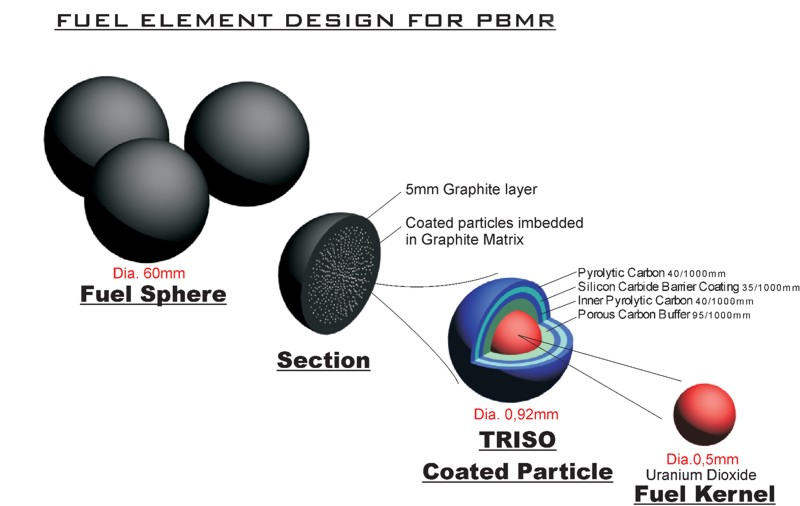
\includegraphics[width=0.85\textwidth]{./images/design/TMSR_fuel.jpg}
  \caption{Schematic of fuel pebbles and triso particles}
  \label{fig:triso}
\end{figure}

The question of how to model the complex geometry of the flow passage in a pebble bed has been tackled in chemistry engineering\cite{Dixon2001}\cite{Miroliaei2011} for fixed bed reactors in chemical processes and in nuclear engineering for analyzing advanced pebble bed reactor designs.  One-dimensional heat conduction simplification is often used in LWR fuel rods and can be used in spherical fuel elements for FHRs for quick scope analysis, but is inadequate for detailed investigation because it ignores temperature gradients in the axial and the radial direction, which can be significant in a FHR core. Two main approaches for full core CFD modeling are realistic modeling and porous media modeling. Realistic modeling has been used to model flow passage directly in a segment of pebbles, from several to several hundreds\cite{Lee2007}\cite{Hassana}\cite{Shams2013}, but quickly becomes unfeasible for a large number of pebbles with the current computation resources. In addition, although the goal of realistic modeling is to model the flow passage realistically, it is not free of assumptions\cite{Lee2007}, e.g. pebble packing structure and contact point treatment. The porous media approach, on the other hand, computes only the average flow conditions with ten time less mesh grids. Comparisons between the direct CFD and porous media methods\cite{Wu2010} suggest that porous media methods provide similar averaged pressure and temperature gradient across the pebble bed to the realistic approach, given the appropriate Darcy-Forchheimer drag model is used. Porous media approach has been used in standard HTR modeling tools Thermix\cite{Struth1985} and Tinte\cite{Gerwin1987}, as well as in a thermal-hydraulics model for FHR\cite{Scarlat2012}.
Appropriate safety margin should be applied in the design given the fact that porous media models do not capture local vertices, flow separation, variations in flow induced heat transfer around the pebble surface and the resulting local hot spots.

Previously, researchers have developed separate codes in thermal-hydraulics\cite{Scarlat2012} and neutronics\cite{Cisneros2013} for FHRs. These codes can be coupled for multiphysics computation using the operator-split method: solving one equation system at a time and transfer data between the codes after each iteration until the results converge. However, the operator split method requires small time steps to ensure convergence due to nonlinear inconsistency\cite{Ragusa2009} and could require a substantial amount of computational resource. This work explores methodology for developing fully coupled neutronics and thermal-hydraulics models for pebble bed FHRs.  


The rest of the paper is organized as following: The methodology, including governing equations, generation of cross-sections and implementation in COMSOL is discussed in section \ref{sec:methodology}. A case study based on TMSR design is then presented in section \ref{sec:res}, as well as verification procedures against a reference model. Future needs are identified in the conclusion.

\section{Methodology}
\label{sec:methodology}

\subsection{Neutronics}
Multi-group diffusion equation provides a good balance between CPU cost and accuracy, and is used in the multiphyscis model for neutronics computation. The governing equations of multi-group neutron diffusion with delayed neutrons are written as following:
  \begin{equation}
    \frac{1}{v_g}\frac{\partial \phi_g}{\partial t} =& \nabla D_g \nabla \phi_g - \Sigma_{t,g}\phi_g + \sum_{g'=1}^{G} \Sigma_{s, g'g}\phi_{g'} + \\\nonumber & \ (1-\beta)\chi_{p,g}\sum_{g'=1}^G(\nu \Sigma_f)_{g'} \phi_{g'} + \chi_{d,g}\sum_{i=1}^D \lambda_iC_i
    \label{eq:diffusion}
  \end{equation}

\begin{equation}
    \frac{\partial C_i}{\partial t} = -\lambda_i C_i + \beta_i \sum_{g=1}^G (\nu \Sigma_f)_g \phi_g 
  \label{eq:delayed_neutrons}
\end{equation}
%
where the quantities are defined as follows:
\\
$v_g$ = neutron speed of the $g$-$th$ group, m/s
\\
  $\Sigma_{s, gg'}$ = macroscopic scattering cross-section from group $g'$ to group $g$, m$^{-1}$
\\
  $\nu$ = mean number of neutrons generated per fission
\\
$\Sigma_{f,g}$ = macroscopic fission cross-section of group $g$, m$^{-1}$
\\
  $\chi_g$ = fraction of delayed ($d$) or prompt ($p$) neutrons from fission generated in group $g$ 
\\
  $\phi_{g}$ = neutron flux in the $g$-$th$ energy interval [$E_g$, $E_{g-1}$], m$^{-2}$s$^{-1}$
\\
  %\begin{align}
  %  \phi_g(r,t) = \int^{E_{g-1}}_{E_g} \phi(r,E,t) dE
  %\end{align}
  $\Sigma_{t,g}$ = macroscopic total cross-section in group $g$, m$^{-1}$
\\
%  \begin{align}
%    \Sigma_{t,g} = \frac{1}{\phi_g}\int_g\Sigma_t(E)\phi(E)dE
%  \end{align}
%
  $D_g$ = diffusion coefficient for energy group $g$, m
\\
  $\beta_i$ = delayed neutron fraction for delayed neutron precursor group $i$
\\
  $\lambda_i$ = average decay constant of delayed neutron precursors, s$^{-1}$
\\
  $C_i$ = delayed neutron precursors concentration
 \\
 G = total number of energy groups\\
 D = total number of delayed neutron precursors groups.
  
  %\begin{align}
  %  D_g = \frac{1}{\phi_g}\int_gD(E)\phi(E)dE = \frac{1}{3\phi_g}\int_g\frac{1}{\Sigma_{tr}(E)}\phi(E)dE
  %\end{align}

%\textbf{Eigenvalue Neutron Diffusion Equation}

For criticality calculations, the effective multiplication factor \keff is inserted into the neutron balance equation to represent the variation of neutron population from one generation to the following one, resulting in:
  \begin{align}
    0 =& \nabla D_g \nabla \phi_g - \Sigma_{a,g}\phi_g - \sum_{\substack{1\\g'\neq g}}^G \Sigma_{s, gg'}\phi_{g} + \\\nonumber &\sum_{\substack{1\\g'\neq g}} \Sigma_{s, g'g}\phi_{g'} + \frac{\chi_{t,g}}{k_{\mathrm{eff}}}\sum_{g'=1}^G(\nu \Sigma_f)_{g'} \phi_{g'}
  \end{align}



A vacuum boundary condition is applied at the outer surfaces. And a symmetry boundary condition is used at the core center-line in 2-D axi-symmetrical models.



\subsubsection{Cross-section generation}
The group-averaged and component-wise neutronic constants are generated with the Monte Carlo neutron transport code SERPENT\cite{Serpent2015}, using the nuclear data library ENDF/B-VII.0.  
Serpent can model packed pebbles and TRISO particles explicitly as the way they are manufactured with the locations given by Discrete Element Method(DEM) computation, although studies\cite{Fratoni2007} have shown that the packing configuration does not affect the results, provided the packing fraction is preserved when pebbles near the wall are cut arbitrarily by the geometry definition. 

A MATLAB package is developed to automatically read data from Serpent output files and produce temperature/density dependent functions for neutronics parameters of as many neutron energy groups as deemed necessary. Currently, an eight-group structure(Table \ref{tab:egroup}) is used to capture the resonance features in cross sections of the major isotopes: U-235, U-238, and those in flibe (shown in Figure~\ref{fig:xs_isotope}).
\begin{figure}[h]
  \centering
  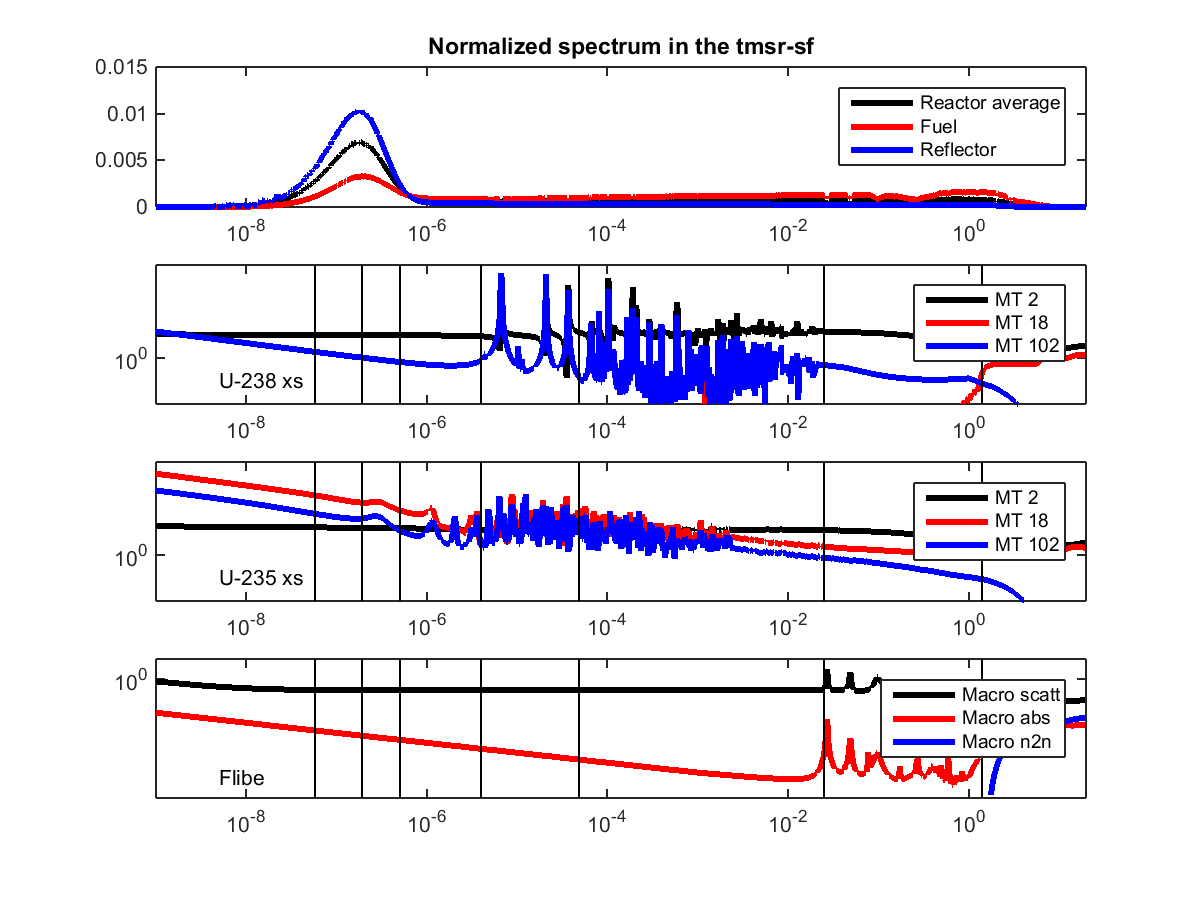
\includegraphics[width=0.8\textwidth]{./images/diffusion/isotope_XS.png}
  \caption{Cross sections of major isotopes in the core.}
  \label{fig:xs_isotope}
\end{figure}

\begin{table}
\caption{Energy group structure adopted in the multi-group neutron diffusion model.}
  \centering
  \begin{tabular}{cc}
  Group \# & Upper energy bound, MeV\\
  \hline
  1 & 20.E+00\\
  2 & 1.4E+00\\
  3 & 2.5E-02\\
  4 & 4.8E-05\\
  5 & 4.0E-06\\
  6 & 5.0E-07\\
  7 & 1.9E-07\\
  8 & 5.8E-08\\
  \hline
  \end{tabular}
  \label{tab:egroup}
\end{table}

As shown in Equation \ref{eq:xs_fuel}, temperature dependent cross-sections of the fuel are modeled as log-linear function because the temperature feedback from the fuel is essentially due to Doppler broadening that has a logarithmic dependence on temperature. The temperature/density dependent cross-sections of the flibe are modeled as linear function of the liquid density because the temperature reactivity feedback in the flibe coolant is mainly due to thermal expansion of the liquid and the linear relationship between the density and the macroscopic cross sections.
% The data are calculated at five different fuel temperatures (300K, 600K, 900K, 1200K, 1500K) and five different flibe densities (17, 18, 19, 20, and 21 kg/m$^3$). 

\begin{equation}
  \Sigma(T_{fuel}) = c_0 + c_1log(T_{fuel}/T_0)
\label{eq:xs_fuel}   
\end{equation}

\begin{equation}
  \Sigma(T_{flibe}) = c_0 + c_1(\rho_{flibe} - \rho_0)
\label{eq:xs_flibe}   
\end{equation}

$c_0$ and $c_1$ are constant coefficients that can be determined by regression analysis.






\subsection{Thermal-hydraulics}
Full core direct CFD modeling of the flow passage formed by more than 10000 pebbles is not practical with current computation capacity. Porous media model requires considerably less computational resource and is used in the multi-physics model.

An important parameter for porous media is the porosity, $\epsilon$, defined as the ratio between the volume of the void to the total volume(Equation \ref{eq:pf}). It appears in the mass(equation \ref{eq:mass}), momentum(equation \ref{eq:mmtm}) and energy conservation equations(equations \ref{eq:pm_liq} and \ref{eq:pm_sol}) below. Local variation in porosity in a pebble bed, including the drop near the wall due to ordered packing, is not modeled explicitly in the porous media model, but the empirical correlations for pressure loss and heat transfer coefficient incorporate corrections for wall effect.


\begin{equation}
  \epsilon = \frac{V_f}{V_f+V_s}
  \label{eq:pf}
\end{equation}

The mass conservation equation for the fluid phase in porous media is written as:
\begin{equation}
  \epsilon\frac{\partial \rho_f}{\partial t} + \nabla(\rho_fv) = 0
  \label{eq:mass}
\end{equation}

where $\rho_f$ is the fluid density in $kg.m^{-3}$, t time in s and v velocity vector in $m.s^{-1}$

The momentum equation for fluid flow in the pebble bed is written as:
% comsol
\begin{equation}
  \frac{\rho_f}{\epsilon} \left[(u\nabla)\frac{u}{\epsilon} \right] + \rho\nabla u = \nabla \left[ -pI + (\frac{\mu}{\epsilon}(\nabla u - (\nabla u)^T) - \frac{2\mu}{3\epsilon} \nabla u I)\right] - (\frac{\mu}{k} + \beta_F \|u\| + \rho\nabla u) u + F
  \label{eq:mmtm}
\end{equation}

The dependent variable here is the superficial velocity, the velocity that the fluid would flow if the channel is free of the solid medium. It is defined as the ratio between the volumetric flow rate and the effective cross section area of the flow channel(Equation \ref{eq:sv}).
\begin{equation}
  u=\frac{Q}{A}
  \label{eq:sv}
\end{equation}

Other parameters used in equation \ref{eq:mmtm} are:\\
$\rho_f$ = fluid density, kg/m3\\
$\epsilon$ = porosity\\
t = time, s\\
p = pressure, Pa\\
$\mu$ = dynamic viscosity, Pa.s\\
F = body force, $N/m^3$\\
I = identity matrix\\
K = permeability, $m^2$\\
$\beta_F$ = Forcheimer drag coefficient, $kg/m^4$\\

The Forcheimer drag coefficient $\beta_F$ and the permeability K are defined in the COMSOL momentum equation according to pebble bed pressure drop characteristics. 
Various pebble bed pressure drop correlations were investigated in previous studies\cite{Scarlat2012} and compared with experimental data\cite{Kang2010}. The most widely used is the Ergun correlation\cite{Ergun1949} for its wide range of validity in laminar, turbulent and transitional regions, its interpretability and convenient implementation, as well as the satisfactory results it provides. It models the pressure loss in a pebble bed as a weighted sum of the viscous energy loss and the inertial energy loss: 


\begin{equation}
  \frac{dp}{dx} = E_1 \frac{(1-\epsilon)^2\mu u}{\epsilon ^2 d^2} + E_2 \frac{1-\epsilon}{\epsilon^3}\frac{\rho u^2}{d}
  \label{eq:ergun}
\end{equation}



They are defined as in equation \ref{eq:betaf} and \ref{eq:K} so that the pressure drop equation in COMSOL(equation \ref{eq:comsol_dp}) matches the Ergun correlation(equation \ref{eq:ergun}).

\begin{equation}
  \frac{dp}{dx} = \frac{\mu}{K}u + \beta_F u^2
  \label{eq:comsol_dp}
\end{equation}

\begin{equation}
      K = \frac{1}{E_1}\frac{\epsilon^3 d^2}{(1-\epsilon)^2}
      \label{eq:K}
\end{equation}

\begin{align}
  \beta_F = c_F \frac{\rho}{\sqrt{K}}
  \label{eq:betaf}
\end{align}

where $c_F$ is the non-dimensional form of the Forcheimer drag coefficient that can be computed from Ergun correlation coefficients $E_1$ and $E_2$ as:

\begin{equation}
    c_F = \frac{E_2}{\epsilon^{1.5}\sqrt{E_1}}
\end{equation}



The energy equations for fluid and solid phases are given in equations \ref{eq:pm_liq} and \ref{eq:pm_sol}.
\begin{equation}
  \epsilon(\rho c_p)_f \frac{\partial T_f}{\partial t} + (\rho c_p)_f U\nabla T_f = \epsilon k_f \nabla\nabla T_f + \Phi + h_{sf}a(T_s - T_f)
  \label{eq:pm_liq}
\end{equation}

\begin{equation}
  (1-\epsilon)(\rho c_p)_s \frac{\partial T_s}{\partial t} =(1-\epsilon)k_s \nabla\nabla T_s + (1-\epsilon)q + h_{sf}a(T_f - T_s)
  \label{eq:pm_sol}
\end{equation}

In the energy equations, $\rho c_p$ is the volumetric heat capacity in $Jm^3K^{-1}$, $T_f$ and $T_s$ are respectively the fluid temperature and the solid temperature in K, $k_f$ is the fluid thermal conductivity in $Wm^{-1}K^{-1}$, a is the specific surface area in $m^{-1}$, q is the heat generation in $Wm^{-3}$.

In a typical nuclear reactor, 97\% of the energy is deposited in the fuel while the rest is transferred to coolant, reflectors and even shield by long range particles such as neutrons and gammas. 
In the current model, nuclear power is assumed generated inside the solid medium of the fuel region and transferred to the coolant through heat convection. Conservative adiabatic boundary condition is applied at the reflector walls. Reflectors have separate coolant channels to maintain the temperature and temperature in outer layers such as graphite reflectors and stainless steel containment has negligible effect on neutronics behaviour, therefore their temperatures are not computed in the coupled simulation. However, it can be computed using the coupled simulation results as boundary conditions.

In a porous media model, the convective heat transfer between the fuel pebbles and the coolant is computed from empirical correlations, whose validation affects directly the credibility of the results. The Wakao correlation(equation \ref{eq:wakao})\cite{Wakao1979} calculates the convective heat transfer coefficient between pebbles and coolant, with Pr and Re the Prandtl and Reynolds numbers.
The constants in the correlation are obtained from a collection of heat transfer data that are carefully examined and corrected for the axial fluid thermal dispersion coefficients. Even though the experimental data that the correlation used to compute the coefficients do not expand the entire FHR flow conditions, recent experimental measurements in randomly packed pebble bed\cite{Huddar2016} have concluded that the Wakao correlation predicts the heat transfer in the FHR conditions adequately.

\begin{equation}
  Nu = 2 + 1.1 Pr^{1/3}Re^{0.6} 
  \label{eq:wakao}
\end{equation}

The convective heat transfer coefficient can be obtained from the Nussult number, the salt thermal conductivity k and pebble diameter $D_p$ using the relationship in equation \ref{eq:nuh}.

\begin{equation}
  h = \frac{kNu}{D_p}
  \label{eq:nuh}
\end{equation}


Inlet coolant temperature are imposed at the inlet boundary.  This enables modeling of overcooling transient by setting the inlet coolant temperature as a time dependent function. Either flow rate or detailed velocity profile perpendicular to the inlet surface can be imposed as flow straighteners are designed to make sure that the inlet flow is fully developed and the coolant injection channels are designed for prescribed inlet flow conditions.

Zero pressure is set to the outlet surfaces. Slip conditions neglect viscous effects are applied to the walls that contain the fluid.  



\subsection{Implementation of the model}
\label{sec:implementation}

The model is implemented in the COMSOL Multiphysics, a software package that solves systems of PDEs or ODEs using the Finite Element Method (FEM), by finding a solution composed of the sum of the product of shape functions and associated coefficients. 
 
The geometry is represented in COMSOL as a CAD model, on which a mesh is generated by the COMSOL meshing tools.
Mesh quality is crucial for finite element method(FEM) simulation as the FEM approximates the real solution by solving a descretized equation system over a mesh grid. For most geometry, a free tetrahedral mesh suffice. To further improve the mesh quality with limited element number, hexahedrons can be used in cylindrical components to minimize the number of mesh elements. The mesh size is directly linked to computation cost and result accuracy. As the mesh element size goes to zero, the solution converges to the real solution at the cost of almost infinite computational resources. 
To find a mesh with optimal finesse, a refinement study compares meshes with different sizes, and choose the one with the least computational requirement that satisfies the convergence criteria. 

In addition to parameters such as material properties, the code takes temperature dependent cross-section functions as input.

COMSOL provides built-in modules for various physics as well as the possibility for user defined PDEs. Neutron diffusion and $SP_N$ equations are defined in COMSOL through the 'user defined PDEs' interface. The heat transfer and momentum equations are generated directly by COMSOL's porous media and heat transfer models, which were discussed in the previous section.


%(https://www.sharcnet.ca/Software/Ansys/17.0/en-us/help/ans_bas/Hlp_G_BAS3_4.html)

Once the equation system is assembled, the solvers start by searching for the eigenvalue in neutronics equations(Equation \ref{eq:diffusion}) with cross-sections computed from an initial guess of uniform temperatures. 
With the flux distribution found by the eigenvalue solver, a stationary solver computes the temperature distribution in the core by solving the conservation equations in thermal-hydraulics modules. However, an eigenvalue solver evaluate the fluxes and power density values(equation \ref{eq:powerdensity}) on an arbitrary scale, so the power density is normalized onto the operation power in steady state solver , as shown in Equation \ref{eq:scale}.  

\begin{equation}
  \dot{P} = \sum_{g=1}^G \kappa \Sigma_{f,g} \flux _g
  \label{eq:powerdensity}
\end{equation}

\begin{equation}
  \dot{P}_N = \frac{\dot{P}.P_{op}}{\iiint_V{\dot{P}dv}}
  \label{eq:scale}
\end{equation}

where the quantities are defined as follows:\\
$P_{op}$ = operation power, W\\
$\dot{p}$ = volumetric power density, $W/m^3$\\
$\dot{p}_N$ = normalized volumetric power density, $W/m^3$\\
$\kappa$ = mean energy generation per fission, $MeV$\\
$\Sigma_{f,g}$ = macroscopic fission cross-section of group $g$, m$^{-1}$\\
$\flux_{g}$ = neutron flux in the $g$-$th$ energy interval [$E_g$, $E_{g-1}$], m$^{-2}$s$^{-1}$\\
G = total number of energy groups.
 
Another eigenvalue search is then performed with the new cross-section set determined from the temperature distribution in stationary solver solution. 
The two steps are repeated until the results converge, i.e. the \keff differs by less than 1~pcm between two iterations.

At the end of the iteration, the fluxes are scaled so that the volume integration of the power density equals to the operating power of the reactor in simulation. New delayed neutron precursor concentrations are computed from the normalized fluxes. The scaling factors are shown in the following equations:
\begin{equation}
    \flux_{gN} = \flux_g \frac{P_{op}}{\iiint_V{\dot{P}dv}}
\end{equation}

\begin{equation}
      C_{dN} = \frac{\beta_d \sum_{g=1}^G (\nu\Sigma_f)_g \flux_{gN}}{\lambda_d}\\
      = C_d\frac{P_{op}}{\iiint_V{\dot{P}dv}}
\end{equation}

where the quantities are defined as follows:\\
$P_{op}$ = operation power, W\\
$\dot{p}$ = volumetric power density, $W/m^3$\\
$\nu$ = mean number of neutrons generated per fission\\
$\Sigma_{f,g}$ = macroscopic fission cross-section of group $g$, m$^{-1}$\\
  $\flux_{g}$ = neutron flux in the $g$-$th$ energy interval [$E_g$, $E_{g-1}$], m$^{-2}$s$^{-1}$
\\
  $\beta_d$ = delayed neutron fraction for delayed neutron precursor group $d$
\\
  $\lambda_d$ = average decay constant of delayed neutron precursors in group d, s$^{-1}$
\\
  $C_d$ = delayed neutron precursors concentration in group d
 \\
 G = total number of energy groups\\
 D = total number of delayed neutron precursors groups.


Once the flux and neutron precursor concentration are scaled, one can simulate transient behaviour by solving the coupled equation system with time derivative terms using COMSOL's transient solver. Time step size is automatically chosen based on the time derivative of the dependent variables.


FEM solvers discretize the space according to the mesh and construct a linear equation system of the basis functions. 
Solving the system of linear equations is a crucial part and the most computationally demanding part of a simulation, for which COMSOL provides two category of methods: direct solvers( MUMPS, PARDISO, and SPOOLES ) and iterative solvers(e.g.  MUMPS, GMRES, FGMRES).
In principal, direct solvers are easier to set up as they do not need preconditioning but require substantial amount of memory for matrix factorization. Iterative solvers approach the solution gradually and requires significantly less memory, but need problem specific tuning.
For smaller mesh, direct solver is faster because it does not need preconditioning and takes a single stride to the solution. But when the memory requirement approaches the hardware limit, the iterative solver performs better by approaching gradually to the solution.
The choice of solvers and their parameters should depend on the specific applications, but all the solvers should find the same results if enough iteration is given. 

By default, the model is considered converged when the estimated error in the iterative solver is below $10^{-3}$. Whether this is sufficient for our application depends on the requirement on precision. This error also need to be put in perspective of other uncertainties involved in the modeling process, the default tolerance is enough if it is negligible compare to the errors introduced by the input parameters.







\section{Case study}
\label{sec:res}
The above methodolgoy is applied to the 10~MW Thorium Molten Salt Reactor (TMSR) SF-1 pebble-bed reactor\cite{wang2014a} developed at the Shanghai Institute of Applied Physics (SINAP). 

The core measures 285~cm in diameter and 300~cm in height. As shown in Figure~\ref{fig:TMSR}, the TMSR core is composed with three major components: an upper region with fuel pebbles and flibe salt at 40\% packing fraction, a lower region with flibe salt and an outer graphite reflector region. 

During normal operation, the coolant salt enters at the bottom inlet at 0.18 m/s and 672$^{\circ}C$ and flows upward. The thermo-physical properties of the salt have not been as extensively measured as water. This model uses recommanded values from Romatoski's review of Fluoride salt properties\cite{Romatoski2017a}, which are listed in Table~\ref{tab:flibe}. The impact of uncertainties in these parameters on the figures of merit will be evaluated in the future.
Fuel pebbles are slightly buoyant in the salt and therefore fills the upper region, whereas the lower region of the core is left with flibe salt. 11558 fresh pebbles are loaded in the core in SERPENT simulation with DEM until the core is critical. An outer graphite reflector surrounds the fuel and coolant, providing neutron moderation and reflection. Independent coolant channels are implanted in the reflector to maintain its temperature. Thus the reflector does not participate in the temperature feedback during most transients except for those that involves issues in the reflector coolant channels.

\begin{figure}[h]
    \centering
    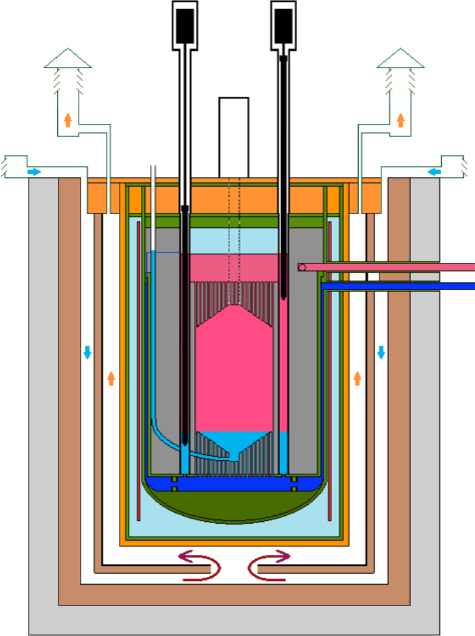
\includegraphics[width=0.6\columnwidth]{./images/design/TMSR_geom.png}
    \caption{Schematic of the TMSR core design and coolant path}
    \label{fig:TMSR}
\end{figure}


\begin{table}
  \caption{Flibe salt thermo-physical properties.}
  \begin{tabular}[h]{lc}
    \hline
    Property & Value\\
    \hline
    Viscosity, kg/m.s & 1.16E-4*e$^{3755/T[K]}$\\
    Heat capacity, J/kg/K & 2386\\
    Thermal conductivity, W/m/K & 1.1\\
    Density, kg/m$^3$ & 2413 - 0.488T[K]\\
    \hline
  \end{tabular}
\label{tab:flibe}
\end{table}

Tiny fuel kernel that is surrounded by four layers in a TRISO particle: a porous graphite layer that buffers the stress from gaseous fission product release and nuclear radiation induced deformation, two pyrolytic carbon layers and a silicon carbide layer to enhance structural strength and prevent radioactive release.  These particles and graphite matrix form a sphere, which is then protected by a graphite shell. 




Coupled heat transfer and neutron diffusion equations are solved with homogenized material properties for each region. Coolant and fuel thermophysical properties are presented in table \ref{tab:flibe}, table \ref{tab:TRISO_prop} and table \ref{tab:pb_prop}. The group constants and delayed neutron parameters are generated from a Serpent model for the TMSR SF-1 core (figure \ref{fig:serpent}) with explicit representation of randomly packed TRISO particles and fuel pebbles. The nuclear data library ENDF/B-VII.0 was used for Monte Carlo neutron transport. 
An eight-group energy structure was chosen with the boundaries shown in table \ref{tab:egroup} to capture the cross section features of the major isotopes: U-235, U-238, and those in flibe(shown in figure \ref{fig:xs_isotope}). 

\begin{table}
  \caption{Dimensions and material properties of each layer of TRISO particles.}
  \begin{tabular}[h]{lccccc}
    \hline
    Region&Material&Thickness/Radius,&Density,&Conductivity,&Specific heat,\\
    &&$10^{-6}$ m&kg/m$^3$&W/m/K&J/kg/K\\
    \hline
    Kernel&19.9\% UC$_{0.5}$O$_{1.5}$&250&10,500&3.5&400\\
    Buffer&porous carbon&95&1,000&0.5&2,000\\
    IPyC&pyrolytic carbon&40&1,900&4.0&2,000\\
    SiC&silicon carbide&35&3,200&30&1,300\\
    OPyC&pyrolytic carbon&40&1,900&4.0&2,000\\
    \hline
  \end{tabular}
  \label{tab:TRISO_prop}
\end{table}


\begin{table}
  \begin{tabular}[h]{ccccc}
    Region&Material&Thickness/Radius&Density&Conductivity\\
    &&[mm]&[g/cc]&[W/m.k] \\
    \hline\\
    Shell&Graphite&1&10.5&3.5\\
    Fuel&TRISO+graphtie matrix&2&3.2&15\\
  \end{tabular}
  \caption{Dimensions and material properties of each layer of a fuel pebble}
  \label{tab:pb_prop}
\end{table}


\begin{table}
\caption{Delayed neutron fractions and decay constants}
\centering
    \begin{tabular}[h]{lcc}
      group \# & $\beta$ & $\lambda$\\
      \hline\\
      1 & 2.15E-4 & 1.25E-2\\
      2 & 1.12E-3 & 3.18E-2\\
      3 & 1.08E-3 & 1.09E-1\\
      4 & 3.09E-3 & 3.17E-1\\
      5 & 9.07E-4 & 1.35\\
      6 & 3.18E-4 & 8.64\\
      \hline
    \end{tabular}
  \label{tab:delayed_neutrons}
\end{table}


\begin{figure}
  \centering
  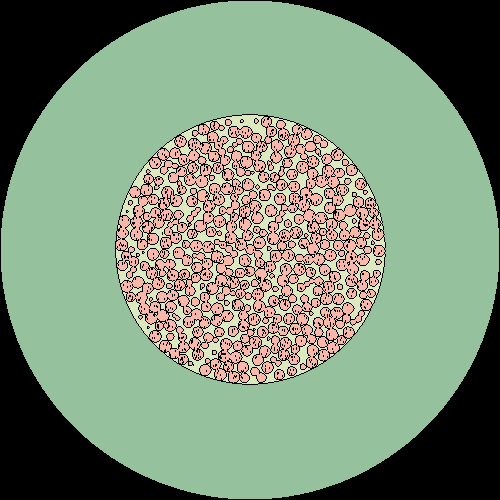
\includegraphics[width=0.5\textwidth]{./images/design/tmsr_sf1_geom1.png}
  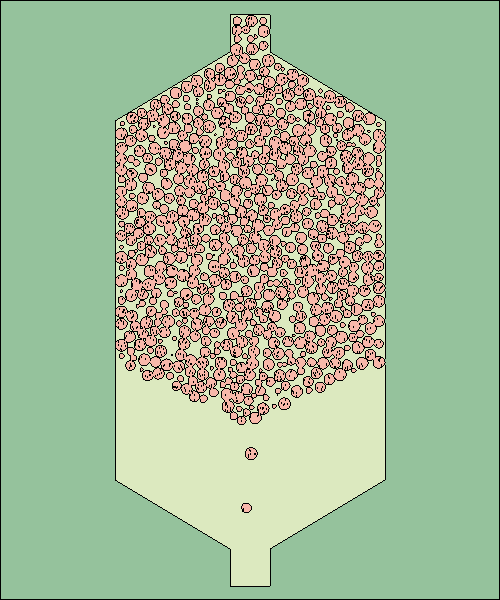
\includegraphics[width=0.415\textwidth]{./images/design/tmsr_sf1_geom2.png}
  \caption{Schematic of the SERPENT model for TMSR}
  \label{fig:serpent}
\end{figure}


\begin{figure}[h]
  \centering
  \begin{subfigure}{0.59\textwidth}
    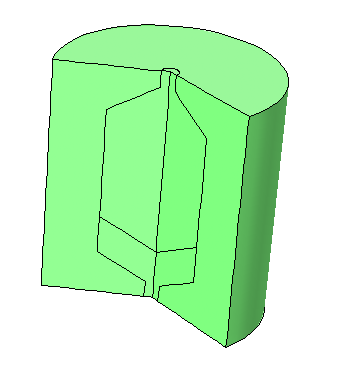
\includegraphics[width = \columnwidth]{./images/diffusion/model_geom.png}
    \caption{Schematic of the TMSR core model geometry}
  \end{subfigure}
  ~
  \begin{subfigure}{0.35\textwidth}
    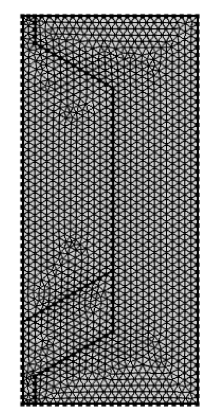
\includegraphics[width = \columnwidth]{./images/diffusion/mesh.png}
    \caption{Schematic of the 2D mesh}
  \end{subfigure}
  \caption{Multi-physics model geometry}
  \label{fig:model_geom}
\end{figure}




\subsection{Mesh refinement study}
The TMSR core model with homogenized regions has a relatively simple geometry(without sharp corners or extreme aspect ratios) and thus the built-in CAD module is used for geometry definition and the default meshing algorithms is used to build meshes with free triangular(2D) or tetrahedral(3D) elements. 

The effect of mesh size on solution accuracy is studied through mesh refinement studies, where the mesh element size is decreased gradually, with the minimum mesh size ranging from 0.1 m to 0.004 m, and the solutions are compared. 
Figure \ref{fig:mesh_refinement} shows the difference in the multiplication factor between a given mesh and the reference. Both quadratic and linear elements are studied. The finest quadratic mesh is used as reference. The plot shows an almost exponential trend between degree of freedom and the computation error. 
Also shown on the plot is that the order of the polynomial functions defined over the mesh elements affects the speed at which the solution converges. This is because FEM method solves the equations by finding a solution composed of the sum of the product of shape functions and associated coefficients. Higher order functions represent the solution with larger flexibility and can approximated the real solution with less elements. 
 
Finer mesh provides more accurate results but also requires more computer resources. One needs to choose the mesh size by balancing the available resource and desirable accuracy. 

\begin{figure}[ht]
  \centering
  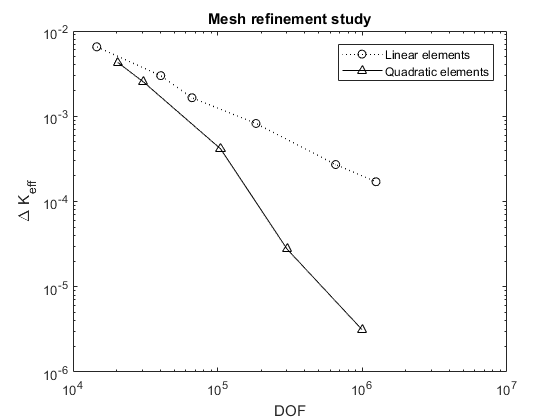
\includegraphics[width = \columnwidth]{./images/diffusion/mesh_refinement.png}
  \caption{Results of mesh refinement study}
  \label{fig:mesh_refinement}
\end{figure}





\subsection{Model verification}
In order to verify the reliability of the COMSOL model, steady state and transient results are compared to a reference model. The reference model\cite{Aufiero2016} uses Serpent for neutron transport and OpenFOAM for CFD modeling. These two codes are internally coupled for best computation performance. To model the reactor core as realistic as possible, the random packing of TRISO particles and fuel pebbles are also simulated, using discrete element method(DEM). The reference model can computes three dimensional distribution of power, temperature, neutron flux, as well as global parameters such as \keff, temperature reactivity feedback coefficients. 
Serpent solves the neutron transport equation in integral form using continuous energy nuclear data with few approximations, therefore it produces valuable reference results for code-to-code verification where experimental data are not available. 


Zero power condition is a good starting point for code-to-code comparison for the neutronics modules as they do not require coupling with thermal-hydraulics. In order to verify the reliability of the neutronic module, the multiplication factor is computed in an isothermal condition, whereby the core is supposed to have a uniform temperature maintained by external heat sources.
 
The first global parameter that is compared is the multiplication factor, the most important global parameter in nuclear reactor control. 
At the nominal condition(flibe density at 1.9~g/cm3 and fuel temperature at 900~K), the multiplication factor from COMSOL and reference model is shown in table \ref{tab:keff}. The error between the COMSOL model and the reference model is much larger than two times of the Monte Carlo statistical error, indicating that the difference is statistically significant. This shows that diffusion based models are inadequate in computing the neutron multiplication factor. However, for transient analysis, which we are most interested in, changes in reactivity when the operation conditions deviates from the reference is more important than the absolute values.
And the time scale and amplitude of these changes are compared in the next sections.

%1051K for flibe
\begin{table}
\centering
  \begin{tabular}{lc}
  \hline
        Code & \keff \\
        \hline\\
       COMSOL & 1.03029  \\
       Reference & 1.08416\\
       $\Delta$\keff & 0.05397\\
       Reference statistical error & 0.00012\\
       \hline
  \end{tabular}
  \caption{Comparison of zero power multiplication factor}
  \label{tab:keff}
\end{table}

The time constant of the system is compared via zero power reactivity insertion transient results. Without temperature reactivity feedback that would stablize the power at a certain level, the reactor power increases exponentially due to excess external reactivity, as shown in equation \ref{eq:pexp}. 

\begin{equation}
P/P_0 =  e^{\rho t/\lambda}
\label{eq:pexp}
\end{equation}
where P is the power, $P_0$ is the initial power, $\rho$ is the reactivity, t is time, and $\lambda$ is the characteristic time constant of the system. 

The speed in which the power ramps up is a direct characteristic of the reactor time scale in the model. As we can see in figure \ref{fig:zero_power}, the results from the COMSOL model match closely to those from the Serpent model for a large range of inserted reactivities. 

\begin{figure}[ht]
  \centering
  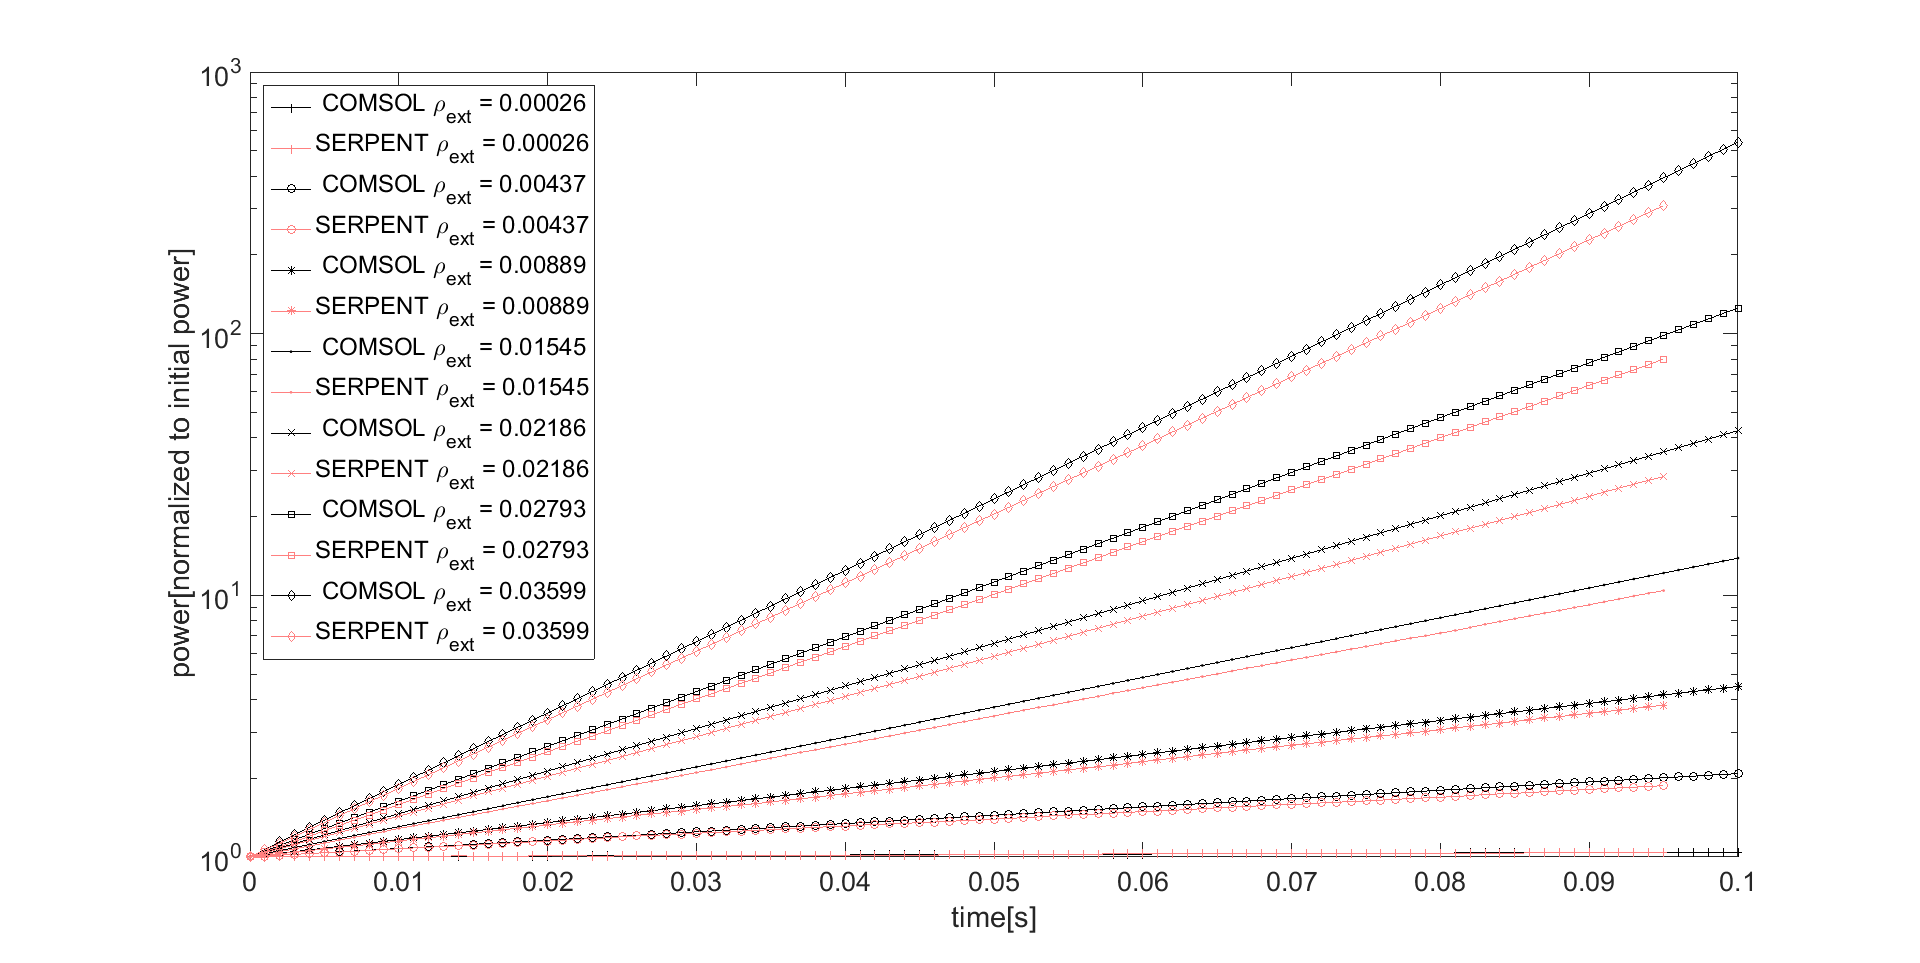
\includegraphics[width=\columnwidth]{./images/benchmark/zero_power_transient.png}
  \caption{Comparison between the diffusion based model and the Monte Carlo based model for zero power reactivity insertion transients}
  \label{fig:zero_power}
\end{figure}


The coupling between neutronics and thermal-hydraulics is manifested on the macroscopic scale as temperature reactivity feedback. The two major ones in FHR, the fuel Doppler feedback and the coolant temperature feedback coefficients, are computed from both models and are compared in figure \ref{fig:fuel_feedback} and \ref{fig:flibe_feedback}. The same y-axis range is used in the two plots for a visual comparison of the order of magnitude of these two feedback mechanisms. The fuel Doppler feedback is the dominant effect in FHR cores. 

In order to compare the variation of reactivity due to temperature change, delta reactivity is compared. It is computed as the difference between the reactivity at a reference temperature(900K for fuel and 1051K for flibe) and at a given temperature. 

The fuel temperature feedback curves agree well. 
The relative error in flibe reactivity feedback is larger but the absolute error is small due to the small magnitude of flibe feedback. And the discrepancy between flibe feedbacks is within statistical errors of the Monte Carlo computation. 


\begin{figure}[ht]
  \centering
  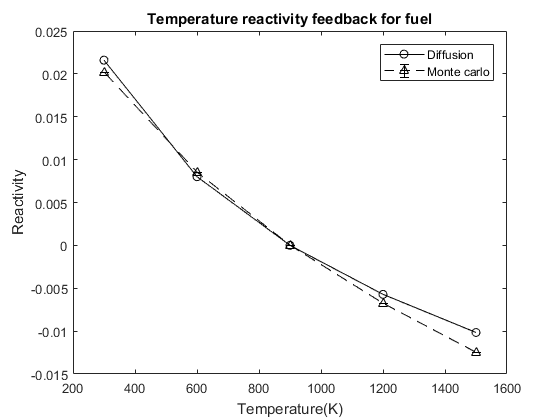
\includegraphics[width=0.8\columnwidth]{./images/benchmark/feedback_fuel.png}
  %\includegraphics[width=0.8\columnwidth]{./images/benchmark/flibe_feedback.png}
  \caption{Comparison between the diffusion based model and the Monte Carlo based model for fuel temperature feedback effect. Error bar shows statistical error in Monte Carlo results.} 
  \label{fig:fuel_feedback}
\end{figure}

\begin{figure}[ht]
  \centering
  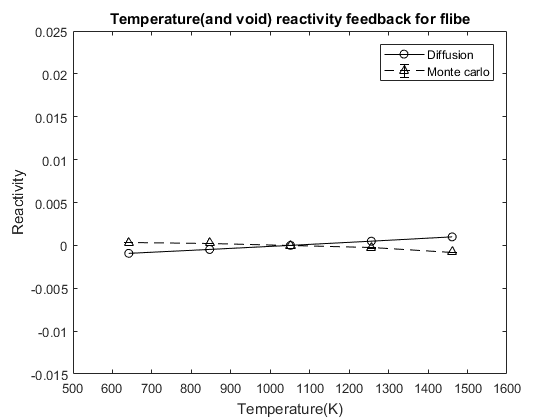
\includegraphics[width=0.8\columnwidth]{./images/benchmark/feedback_flibe.png}
  \caption{Comparison between the diffusion based model and the Monte Carlo based model for flibe temperature feedback effect. Error bar shows statistical error in Monte Carlo results.} 
  \label{fig:flibe_feedback}
\end{figure}


In addition to global parameters, power distribution is also compared. Figure \ref{fig:power_comp} shows the steady state power distribution on a 2~cm x 2~cm mesh, the result from the COMSOL model on the left and that from the reference model on the right, both normalized such that the full core integration is unity. 
Satisfying similarity has been found between the results. The diffusion-based model captures the boundary effect of the reflector adequately despite the fundamental flaw of the diffusion assumption in vicinity of the boundaries. However, because the individual pebbles are not explicitly modeled, the diffusion model cannot represent the local variation in power due to the discrete packing of fuel pebbles. As a result, the power profile seems smoother in the COMSOL model. 

In a randomly packed pebble bed, the porosity is slightly higher at the center and lower at the wall because of the ordering effect. Near the walls, the Monte Carlo result shows a drop in power density due to ordered pattern of pebbles, but this can not be captured by the COMSOL model because it uses homogenized cross sections in the fuel region.

Furthermore, the interface between the fuel pebble region and the flibe region is approximated by a straight line in the COMSOL model. This is different from the randomly packed fuel region in the reference model but can be calibrated for a better match. 


\begin{figure}[ht]
  \centering
  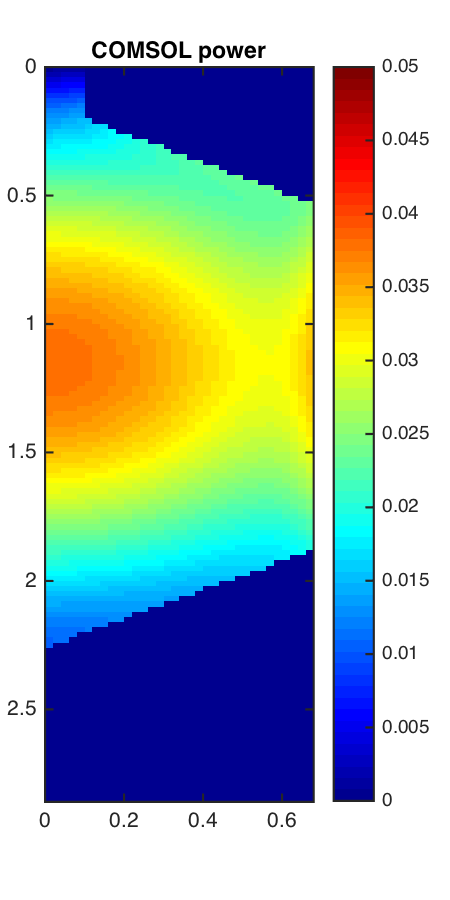
\includegraphics[width=0.3\columnwidth]{./images/benchmark/comsol_power.png}
  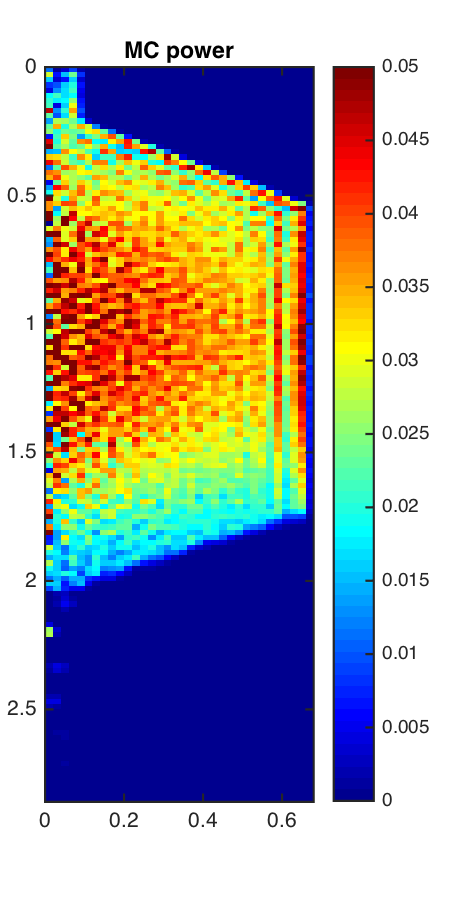
\includegraphics[width = 0.3\columnwidth]{./images/benchmark/MC_power.png}
  \caption{Steady state power profile computed from the COMSOL model and the Monte Carlo reference model}
  \label{fig:power_comp}
\end{figure}
% \begin{figure}[ht]
%   \centering
%   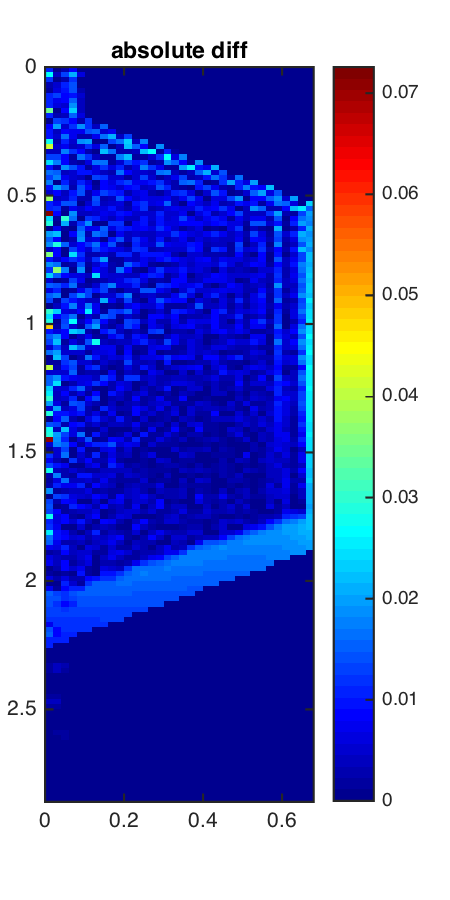
\includegraphics[width=0.3\columnwidth]{./images/benchmark/diff_abs.png}
%   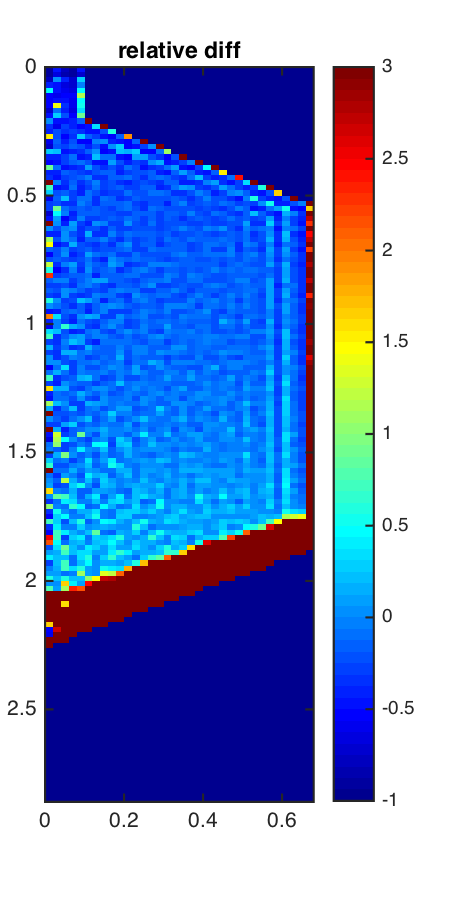
\includegraphics[width = 0.3\columnwidth]{./images/benchmark/diff_rel.png}
%   \caption{Steady state power profile computed from the COMSOL model and the Monte Carlo reference model}
%   \label{fig:power_comp_diff}
% \end{figure}

In addition to the two-dimensional (r, z) profile, the power density is integrated along the axial and radial directions and the resulting axial and radial power distributions are compared respectively in figure \ref{fig:axial_power} and \ref{fig:radial_power}. 
The difference in axial power in figure \ref{fig:axial_power} is mainly due to the approximations in the shape of the fuel region. The most obvious discrepancy is when the power drops to zero at the fuel-flibe interface.
Figure \ref{fig:radial_power} shows the difference in radial power distribution. The step changes in power density along the radius in the reference result is due to the effect of discrete pebble packing, which causes local variations in fuel pebble packing fraction.

\begin{figure}[ht]
  \centering
  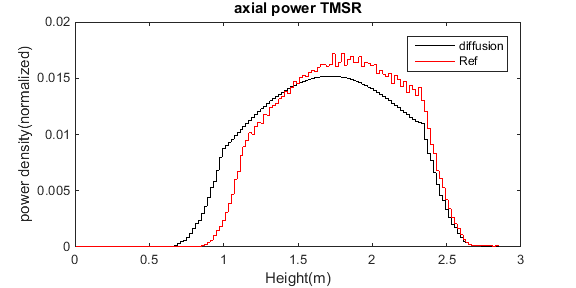
\includegraphics[width=0.9\columnwidth]{./images/benchmark/axial_TMSR.png}
  \caption{Comparison of the axial distribution of normalized power}
  \label{fig:axial_power}
\end{figure}

\begin{figure}[ht]
  \centering
  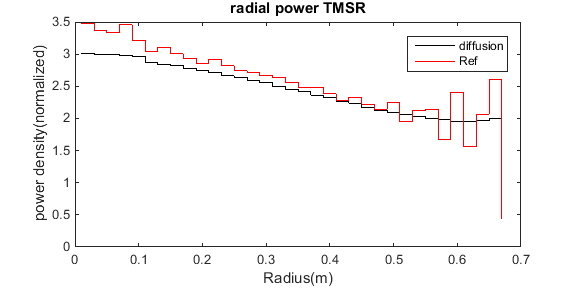
\includegraphics[width=0.9\columnwidth]{./images/benchmark/radial_TMSR.png}
  \caption{Comparison of the radial distribution of normalized power}
  \label{fig:radial_power}
\end{figure}


The multiplication factor is the most important scalar global parameter in nuclear reactor control. In order to verify the reliability of neutronic module in the code in determining the multiplication factor, an isothermal condition is imposed in the core, whereby the core is supposed to have a uniform temperature maintained by external heat sources. 
 
At nominal condition(flibe density at 1.9~g/cm3 and fuel temperature at 900~K), the multiplication factor from COMSOL and reference model is show in table \ref{tab:keff}. The error between the COMSOL model and the reference model is larger than three times of the Monte Carlo statistical error, indicating that the difference is statistically significant with 95\% of confidence. This shows that diffusion based models are inadequate to compute the neutron balance accurately. However, for transient analysis, which we are most interested in, changes in reactivity when the operation conditions deviates from the reference is more important than the absolute values.
The time scale and amplitude of these changes are compared.

%1051K for flibe
\begin{table}
\centering
  \begin{tabular}{lc}
  \hline
        Code & \keff \\
        \hline\\
       COMSOL & 1.03029  \\
       Reference & 1.08416\\
       $\Delta$\keff & 0.05397\\
       Reference statistical error & 0.00012\\
       \hline
  \end{tabular}
  \caption{Comparison of zero power multiplication factor}
  \label{tab:keff}
\end{table}





\subsection{Steady state results}
After careful code-to-code verification for the multi-physics model, parameters such as power, flibe and fuel temperatures, and neutron flux are computed with design parameters in table \ref{tab:tmsr_design}. Uniform temperature and uniform upward velocity are imposed as the inlet boundary condition. Vacuum boundary condition for neutron diffusion is used outside of the reflector.  

% flux
An eight-group energy structure is used in the neutron diffusion equations but the neutron flux values are regrouped into thermal ([0.00E+00, 5.00E-07] MeV) and fast  ([5.00E-07, 1.40E+00] MeV) regions for plotting purpose. As confirmed by the plots, fast neutrons are generated exclusively from nuclear reactions in the fuel region and are then scattered by the matters in the core as they get thermalized. 
The moderation effect of the coolant is dwarfed by that of the graphite reflector in TMSR. As a result, a large portion of thermal neutrons is found inside the reflector, besides the center of the core.

The thermal neutrons that travel back from the reflector to the fuel region cause a peak in power density near the border as they trigger nuclear reactions. 
% power
As shown in figure \ref{fig:tmsr_power_ss}, the power peaks at the center of the fuel region, decreases outward and increases again next to the reflector boundaries due to the moderation effect of the graphite reflector. This confirms that the neutron diffusion based model captures the boundary effect adequately. The radial power peaking in TMSR SF-1 is 1.24 at nominal conditions with fresh fuel.

 

\begin{figure}[h]
  \centering
    \begin{subfigure}[b]{0.3\textwidth}
        \centering
        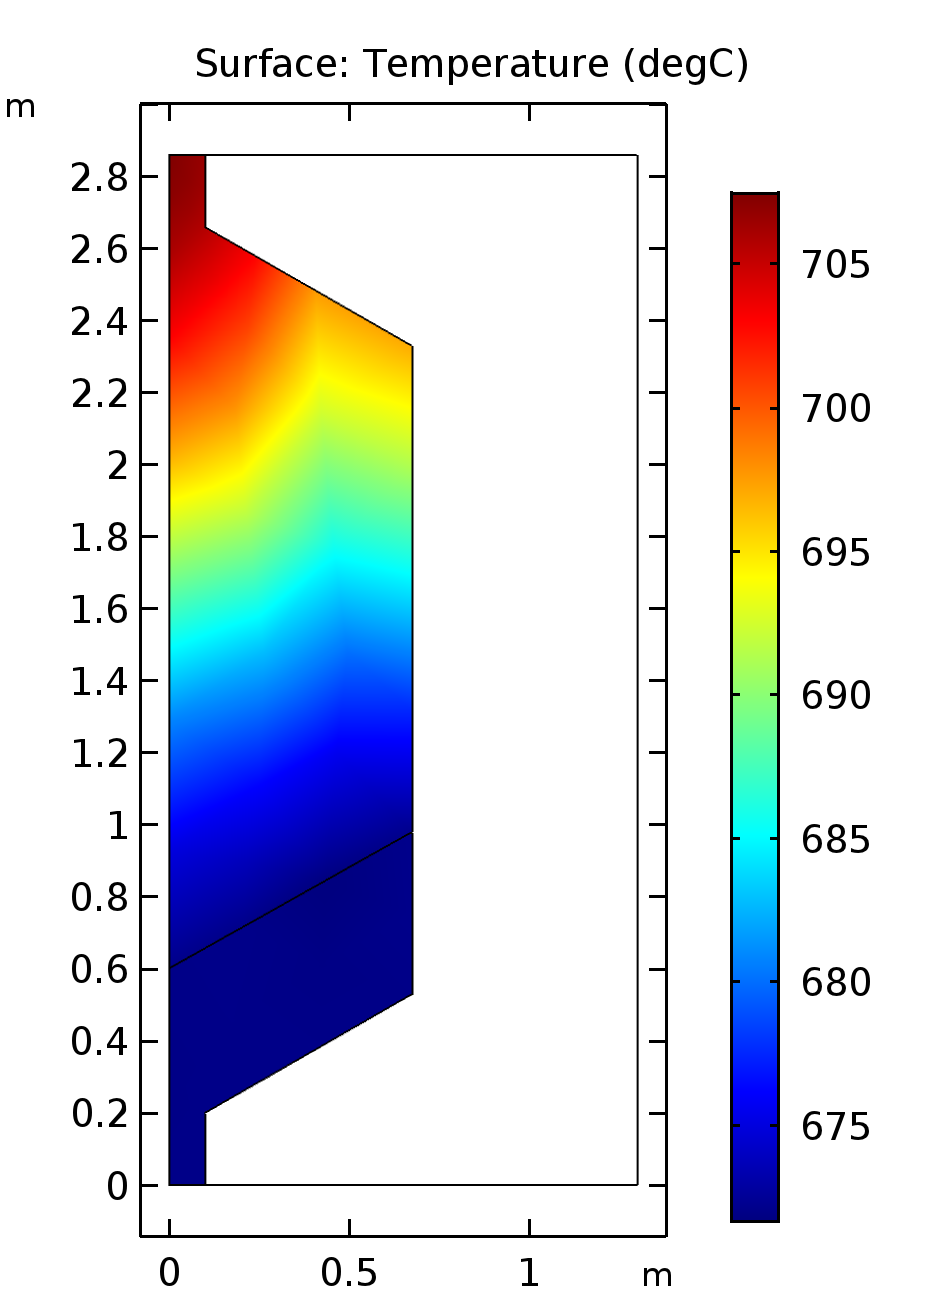
\includegraphics[width=0.9\textwidth]{./images/diffusion/tmsr/SS/non_ms/T_flibe(steady_state).png}
        \caption{Flibe}
    \end{subfigure}%
    ~
    \begin{subfigure}[b]{0.3\textwidth}
        \centering
        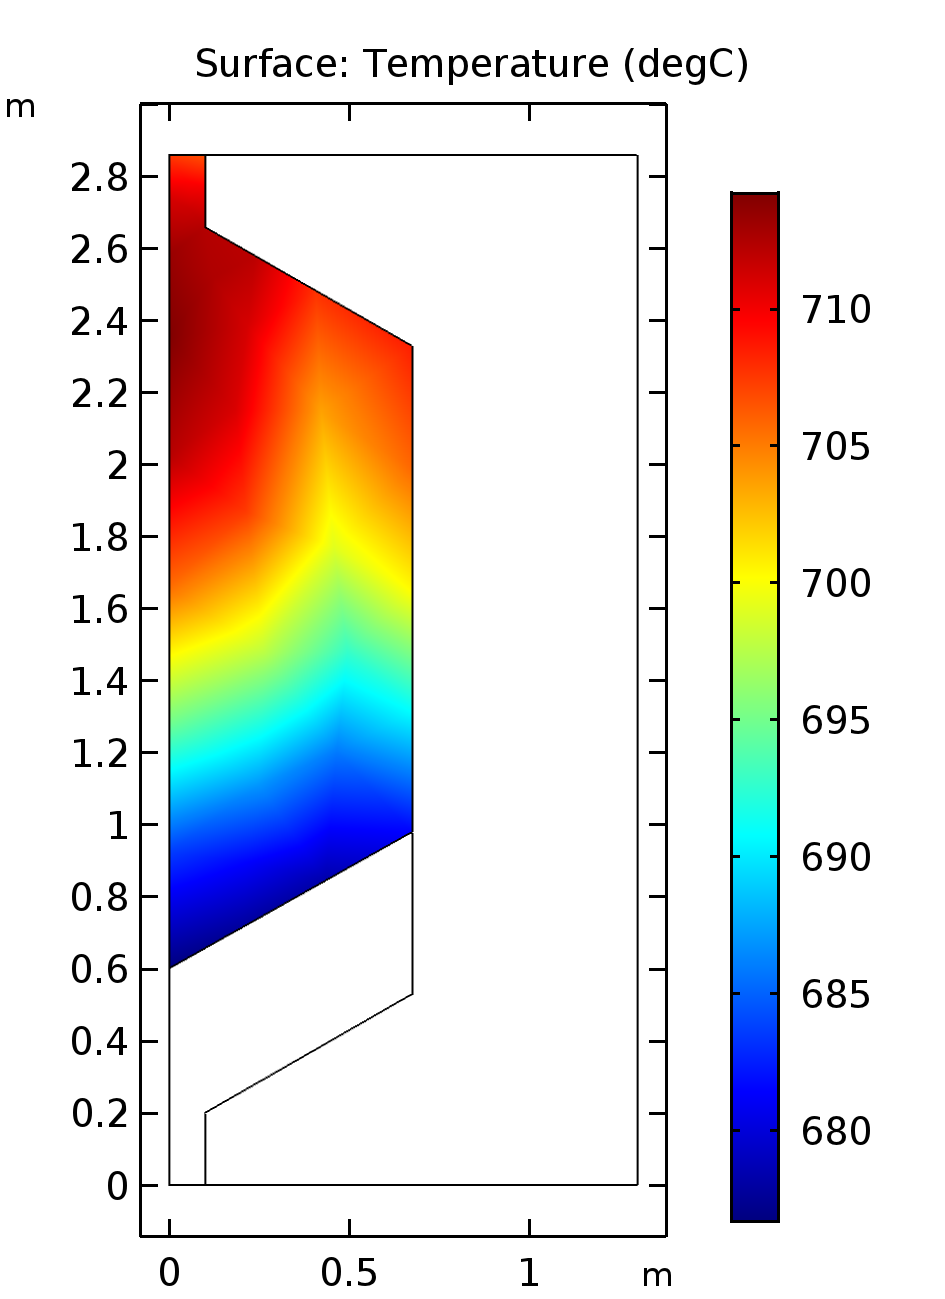
\includegraphics[width=0.9\textwidth]{./images/diffusion/tmsr/SS/non_ms/T_fuel(steady_state).png}
        \caption{Fuel}
    \end{subfigure}

  \caption{Steady state temperatures in TMSR SF-1 core, without multiscale treatment}
  \label{fig:tmsr_temp_non_ms_ss}
\end{figure}

\begin{figure}[h]
  \centering
    \begin{subfigure}[b]{0.3\textwidth}
        \centering
        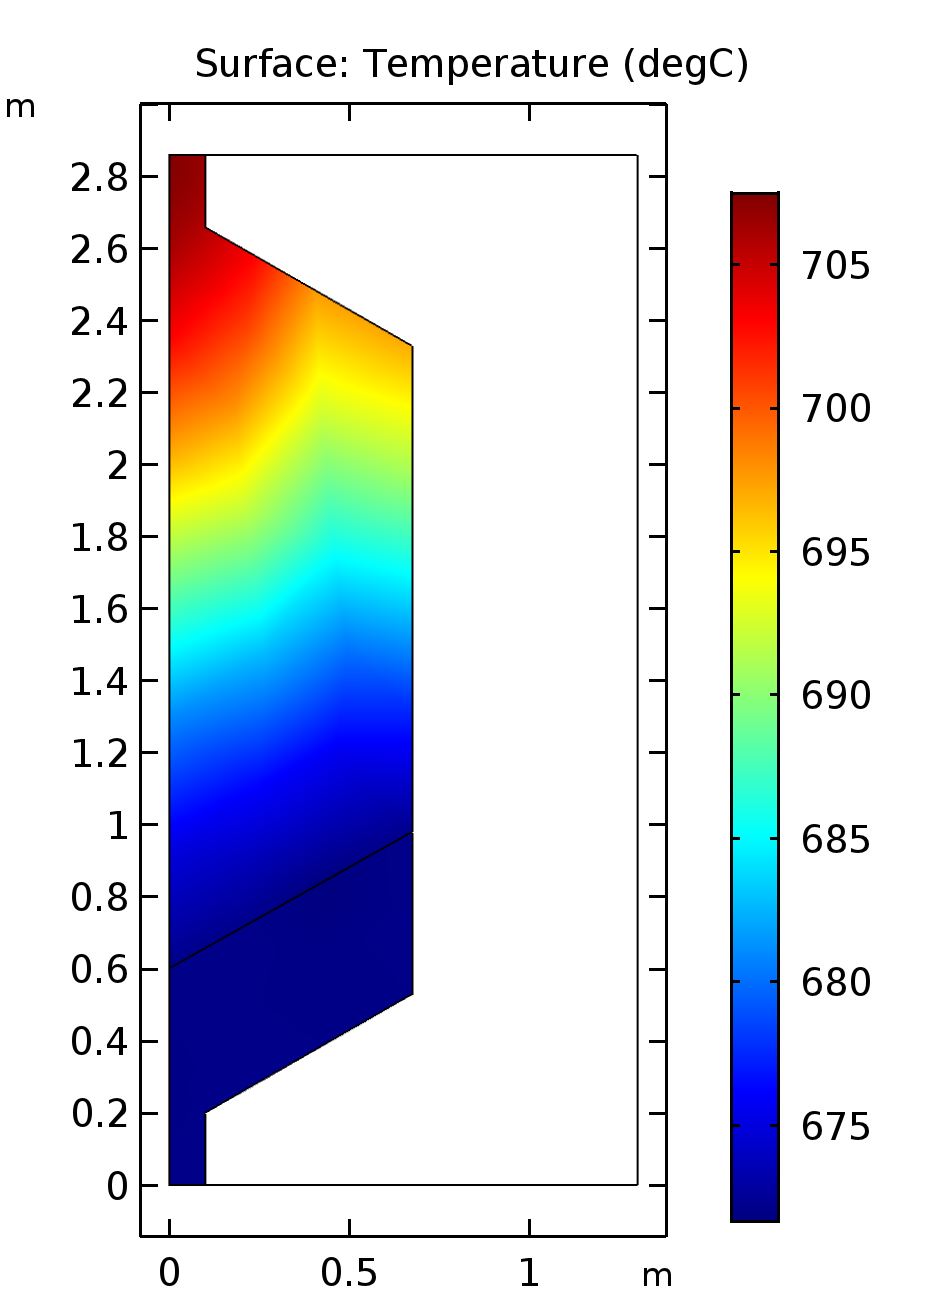
\includegraphics[width=0.9\textwidth]{./images/diffusion/tmsr/SS/ms/T_flibe(steady_state).png}
        \caption{Flibe}
    \end{subfigure}%
    ~
    \begin{subfigure}[b]{0.3\textwidth}
        \centering
        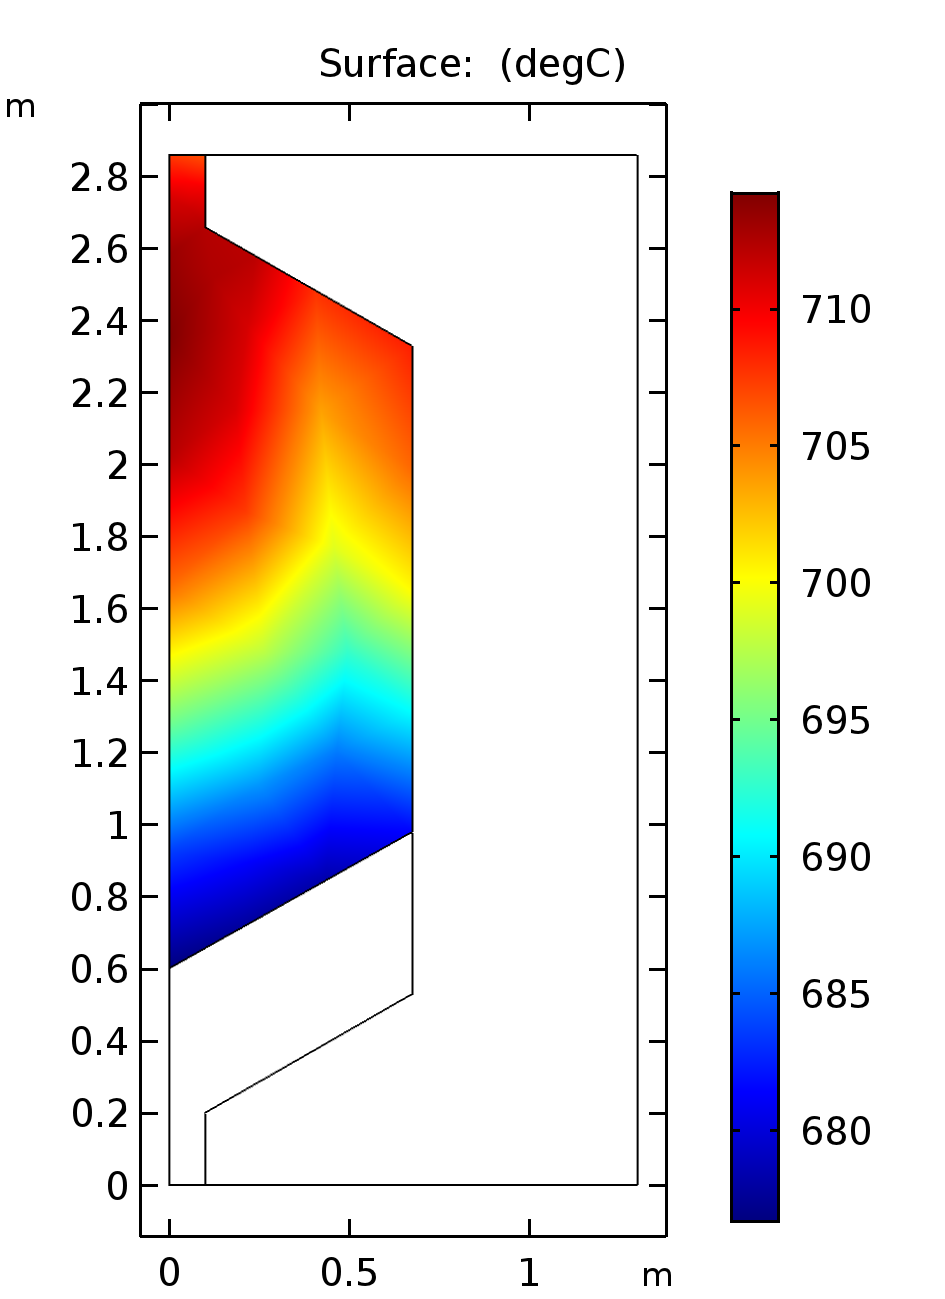
\includegraphics[width=0.9\textwidth]{./images/diffusion/tmsr/SS/ms/T_fuel(steady_state).png}
        \caption{Fuel surface}
    \end{subfigure}
    ~
    \begin{subfigure}[b]{0.3\textwidth}
        \centering
        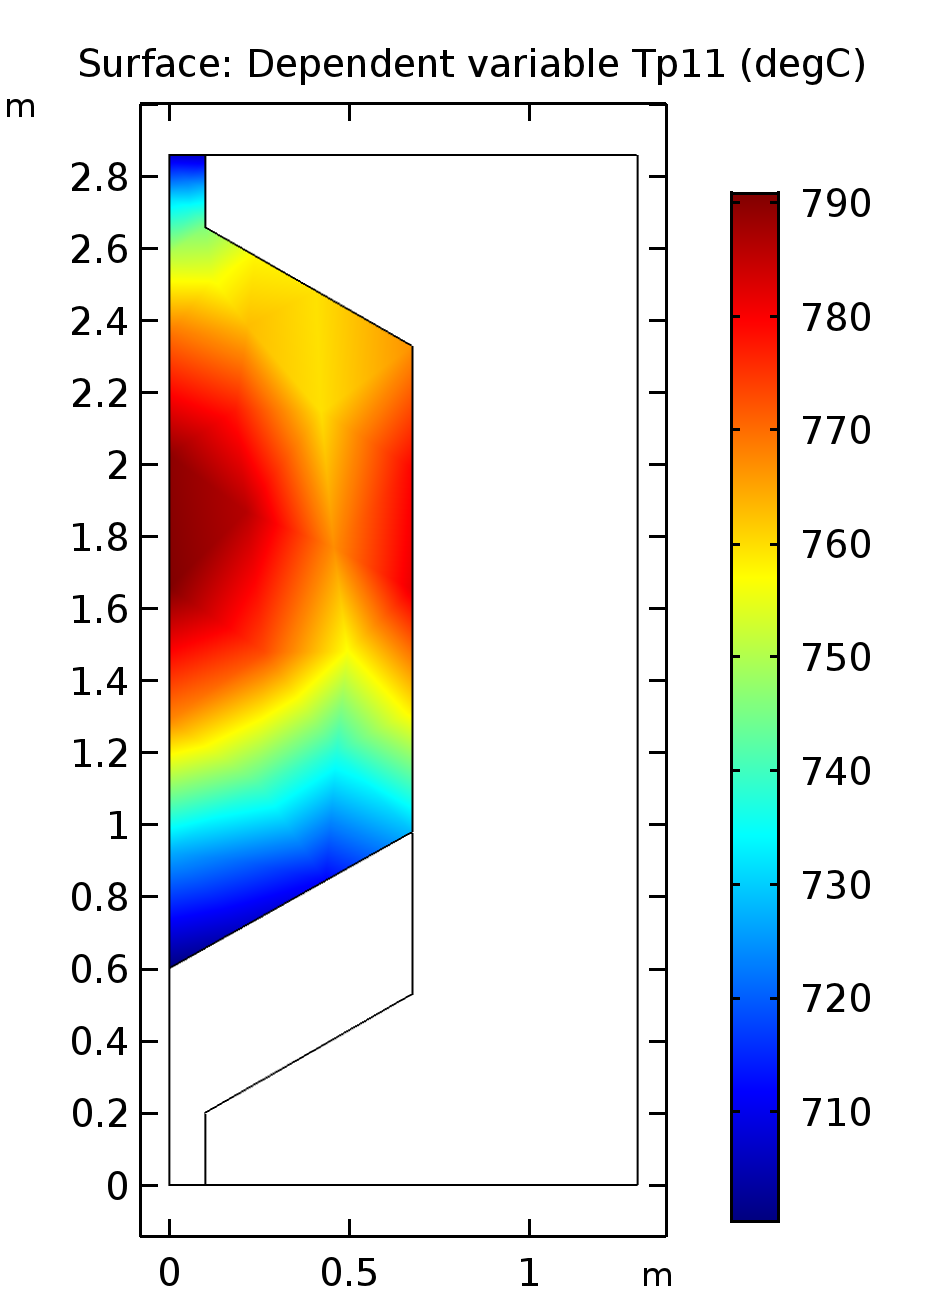
\includegraphics[width=0.9\textwidth]{./images/diffusion/tmsr/SS/ms/Tp11(steady_state).png}
        \caption{Inner TRISO fuel layer}
    \end{subfigure}

  \caption{Steady state temperatures of coolant and selected locations in fuel element in TMSR SF-1 core, with multiscale treatment}
  \label{fig:tmsr_temp_ss}
\end{figure}



The fuel temperature distribution resembles the power profile: hottest in the center and coldest at the two axial extremities, within a range between 1000K and 1120 K. 
The coolant enters the bottom of the core at 672$^{\circ}C$ and gradually heats up to 708$^{\circ}C$ as it flows through the fuel region.
Because of the large volumetric heat capacity of flibe, the coolant is a very efficient heat carrier in TMSR. Both coolant and fuel have large temperature margin below safety limit, which makes TMSR core very robust to transients.

Under the standard porous media model, a fluid temperature and a solid temperature are computed at each two dimensional points in the core. Beyond this, the multiscale treatment in the model tracks the heat transfer inside solid fuel elements and computes a set of temperatures that represents the temperature profile at various depth of the fuel elements. The resulting temperatures with or without the multiscale treatment at steady state are compared in figure \ref{fig:tmsr_temp_ss} and \ref{fig:tmsr_temp_non_ms_ss}.
At steady state, it is assumed that all the nuclear power is generated in the fuel and is transported to coolant and subsequently to the secondary loop through heat exchangers. Therefore, the coolant temperature profile are very similar with or without the multiscale treatment in fuel. 
Because of the large volumetric heat capacity of flibe, the coolant is a very efficient heat carrier in FHRs.
The coolant enters the bottom of the TMSR SF-1 core at 672$^{\circ}C$, as imposed by the inlet boundary condition, and gradually heats up to, on average, 705$^{\circ}C$ as it flows through the fuel region.

Among all the temperatures computed in the solid fuel elements, only the coldest (in the pebble shell) and the hottest (in the center layer of TRISO particles) temperature in a pebble are shown in figure \ref{fig:tmsr_temp_ss} as the upper and lower bound of the solid phase temperatures. The temperature distribution in the center of the TRISO particles resembles the power profile: hottest in the center of the core and coldest at the two axial extremities, within a range between 710 and 790 $^{\circ}C$. 
The surface temperature is, on the other hand, affected both by the nuclear power and by the coolant flowing upward across the core and shifting the peak temperature upward. The hottest fuel surface temperature is attained at the top of the core, where the coolant is the hottest. 


Overall, both the coolant and the fuel are far below their respective safety limits at steady state. The large thermal margins make the TMSR SF-1 core very robust to transient scenarios. 





\section{TMSR SF-1 transient analysis}
\label{sec:TMSR_transients}

To demonstrate the model's capability in simulating transient behaviour and to understand the implication of the multiscale treatment on safety parameters, such as power, coolant temperature and temperature in the solid fuel elements, in comparison to the conventional porous media approach, reactivity insertion and overcooling transients are simulated and the results are discussed in this section. 

In the multiscale case, the average fuel temperature is computed as a volume average of all the solid layers that contains fuel material, i.e. the temperature of graphite layers are not included in the average. This can then be averaged over the two dimensional space to obtain the core average fuel temperature. And in a similar fashion, the core maximum fuel temperature in the multiscale case is the maximum temperature of the hottest power-generating layer, which is the inner-most layer in a TRISO particle that is in the inner-most layer of a fuel pebble at the center of the core. 



\subsection{Reactivity insertion transients}


\begin{figure}
    \centering
    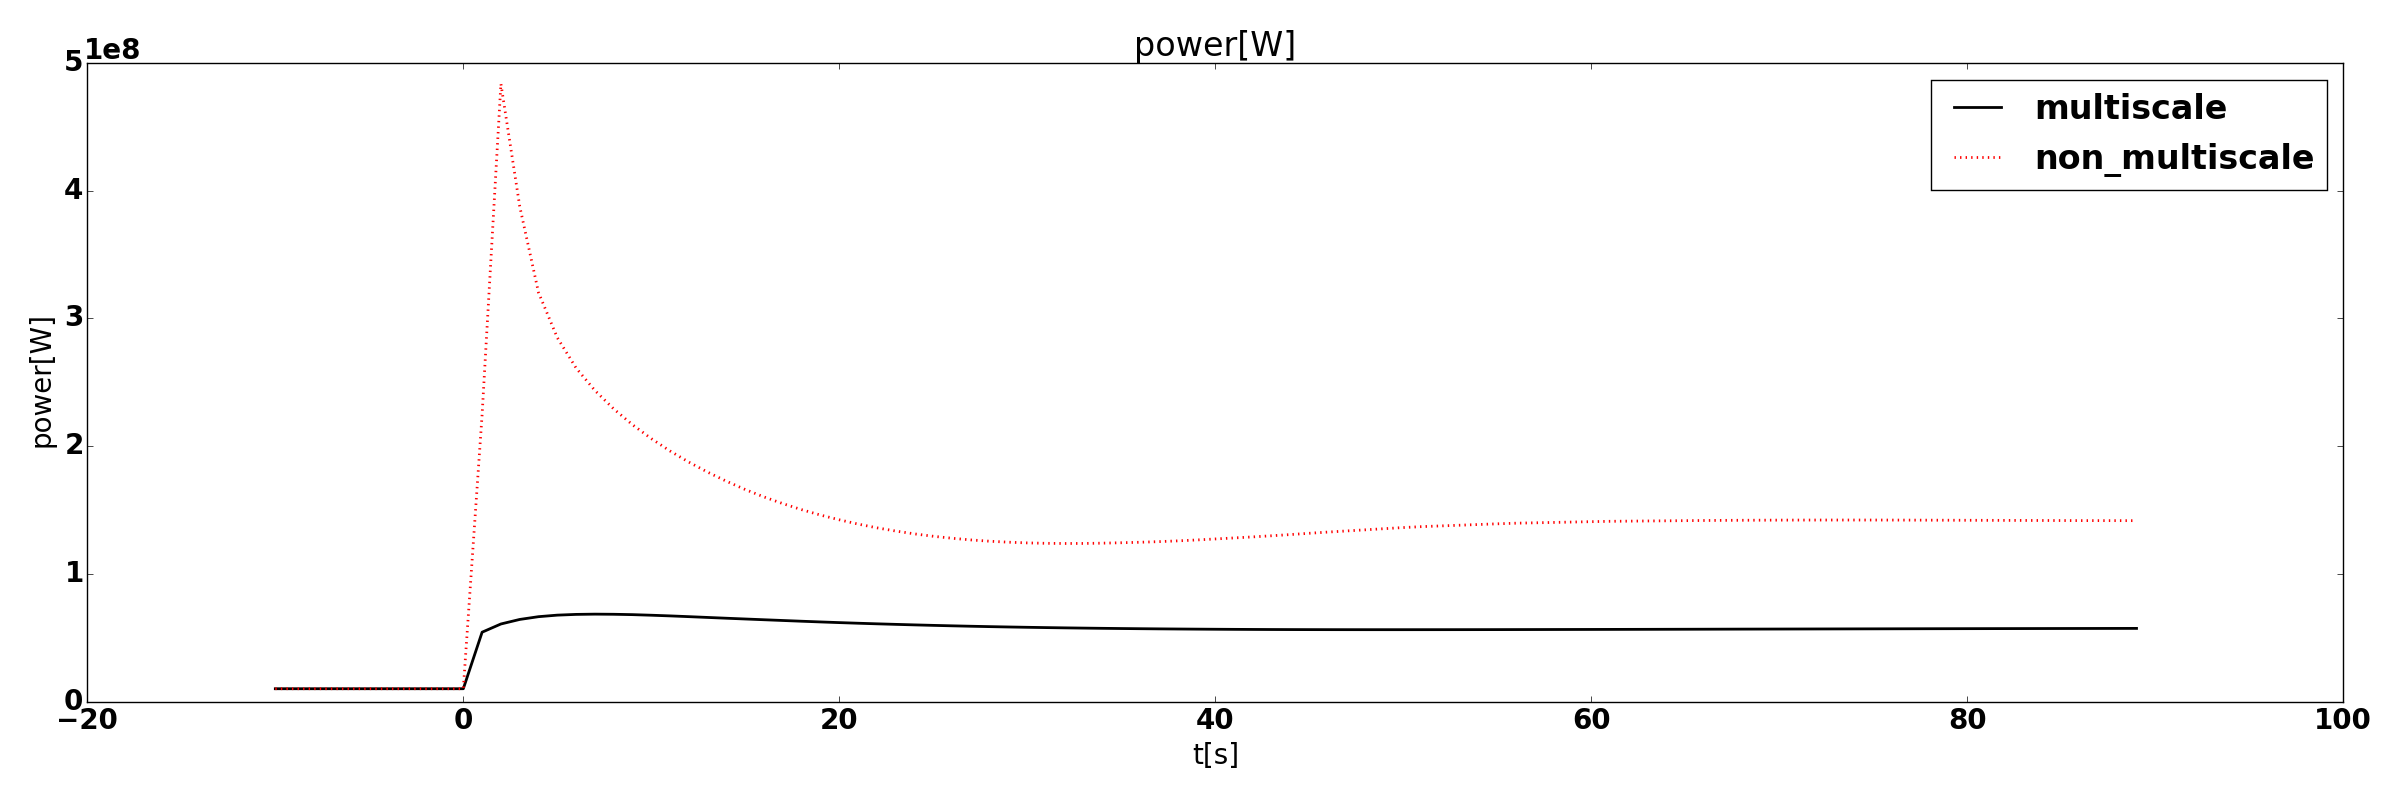
\includegraphics[width=\textwidth]{images/diffusion/tmsr/RI/compare_multiscale/power.png}
    \caption{Full core power during a 1\$ reactivity insertion transient in TMSR SF-1, with or without multiscale treatment}
    \label{fig:multi_comp_power_TMSR}
\end{figure}

\begin{figure}
    \centering
    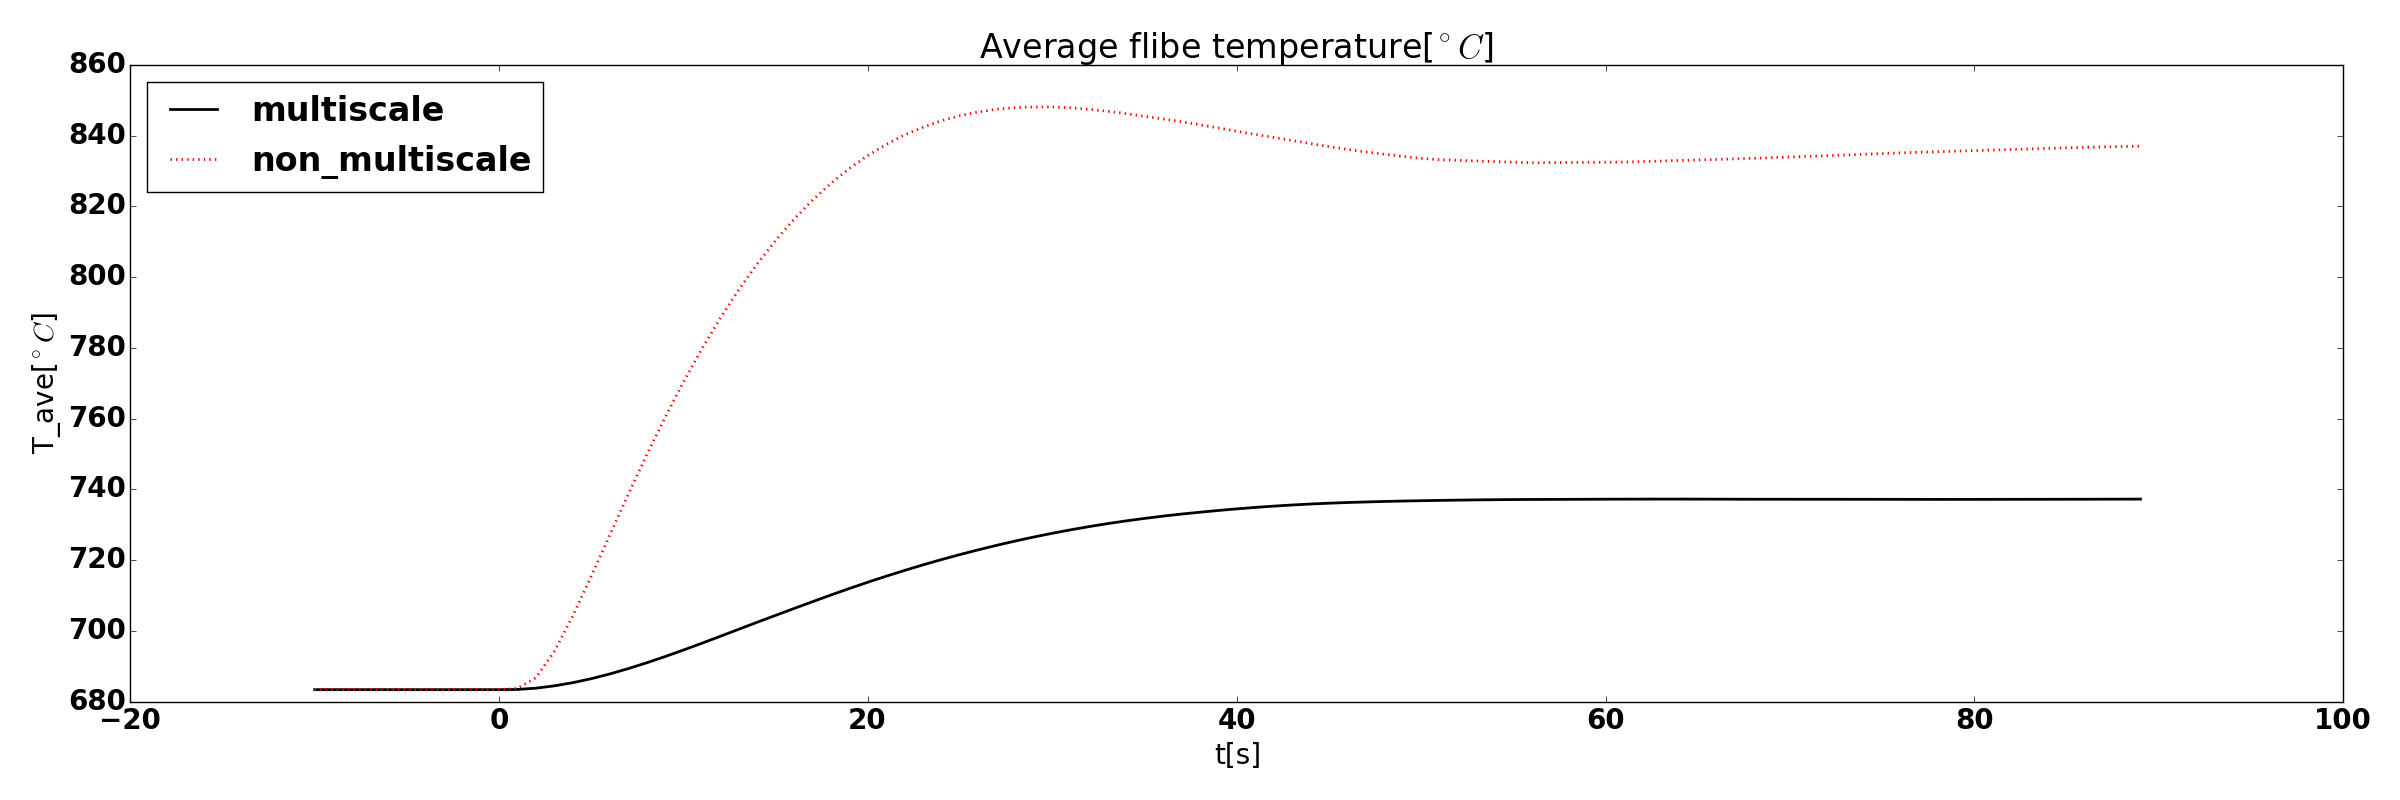
\includegraphics[width=\textwidth]{images/diffusion/tmsr/RI/compare_multiscale/T_flibe_ave.png}
    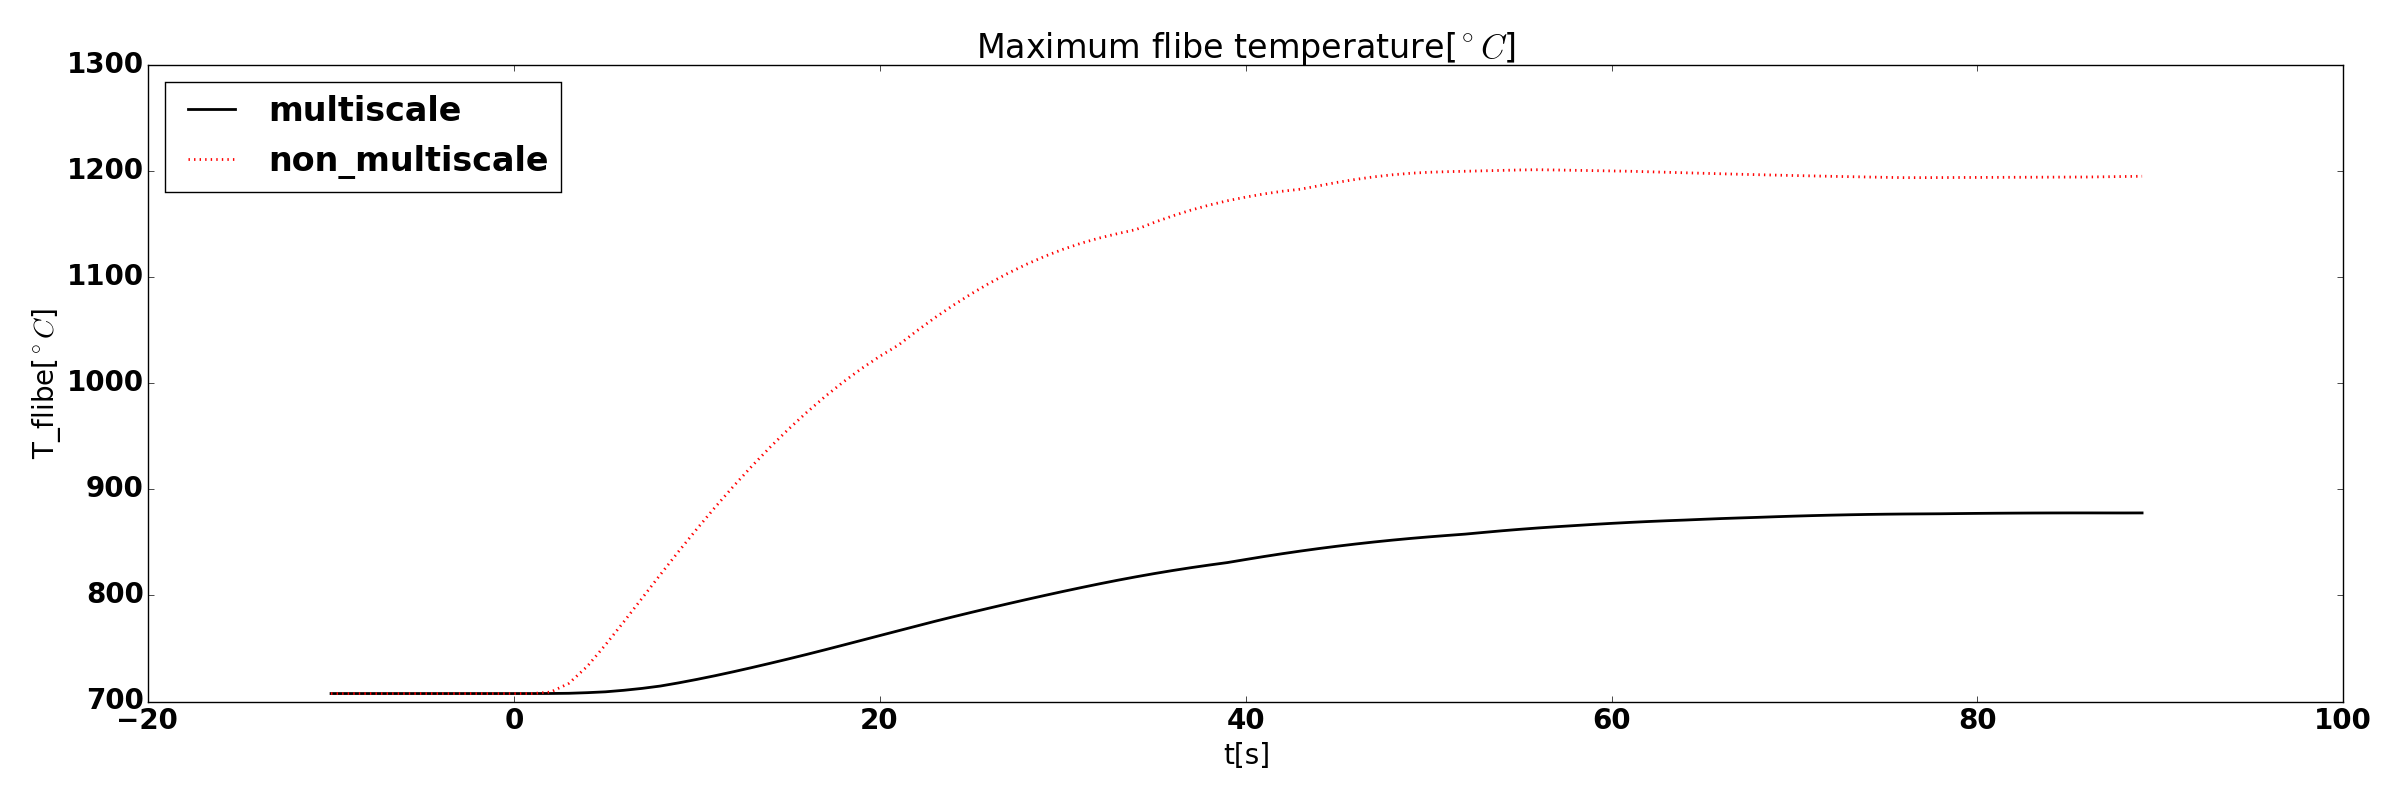
\includegraphics[width=\textwidth]{images/diffusion/tmsr/RI/compare_multiscale/T_flibe_max.png}
    \caption{Average and maximum flibe temperatures during a 1\$ reactivity insertion transient in TMSR SF-1, with or without multiscale treatment}
    \label{fig:multi_comp_flibe_TMSR}
\end{figure}

\begin{figure}
    \centering
    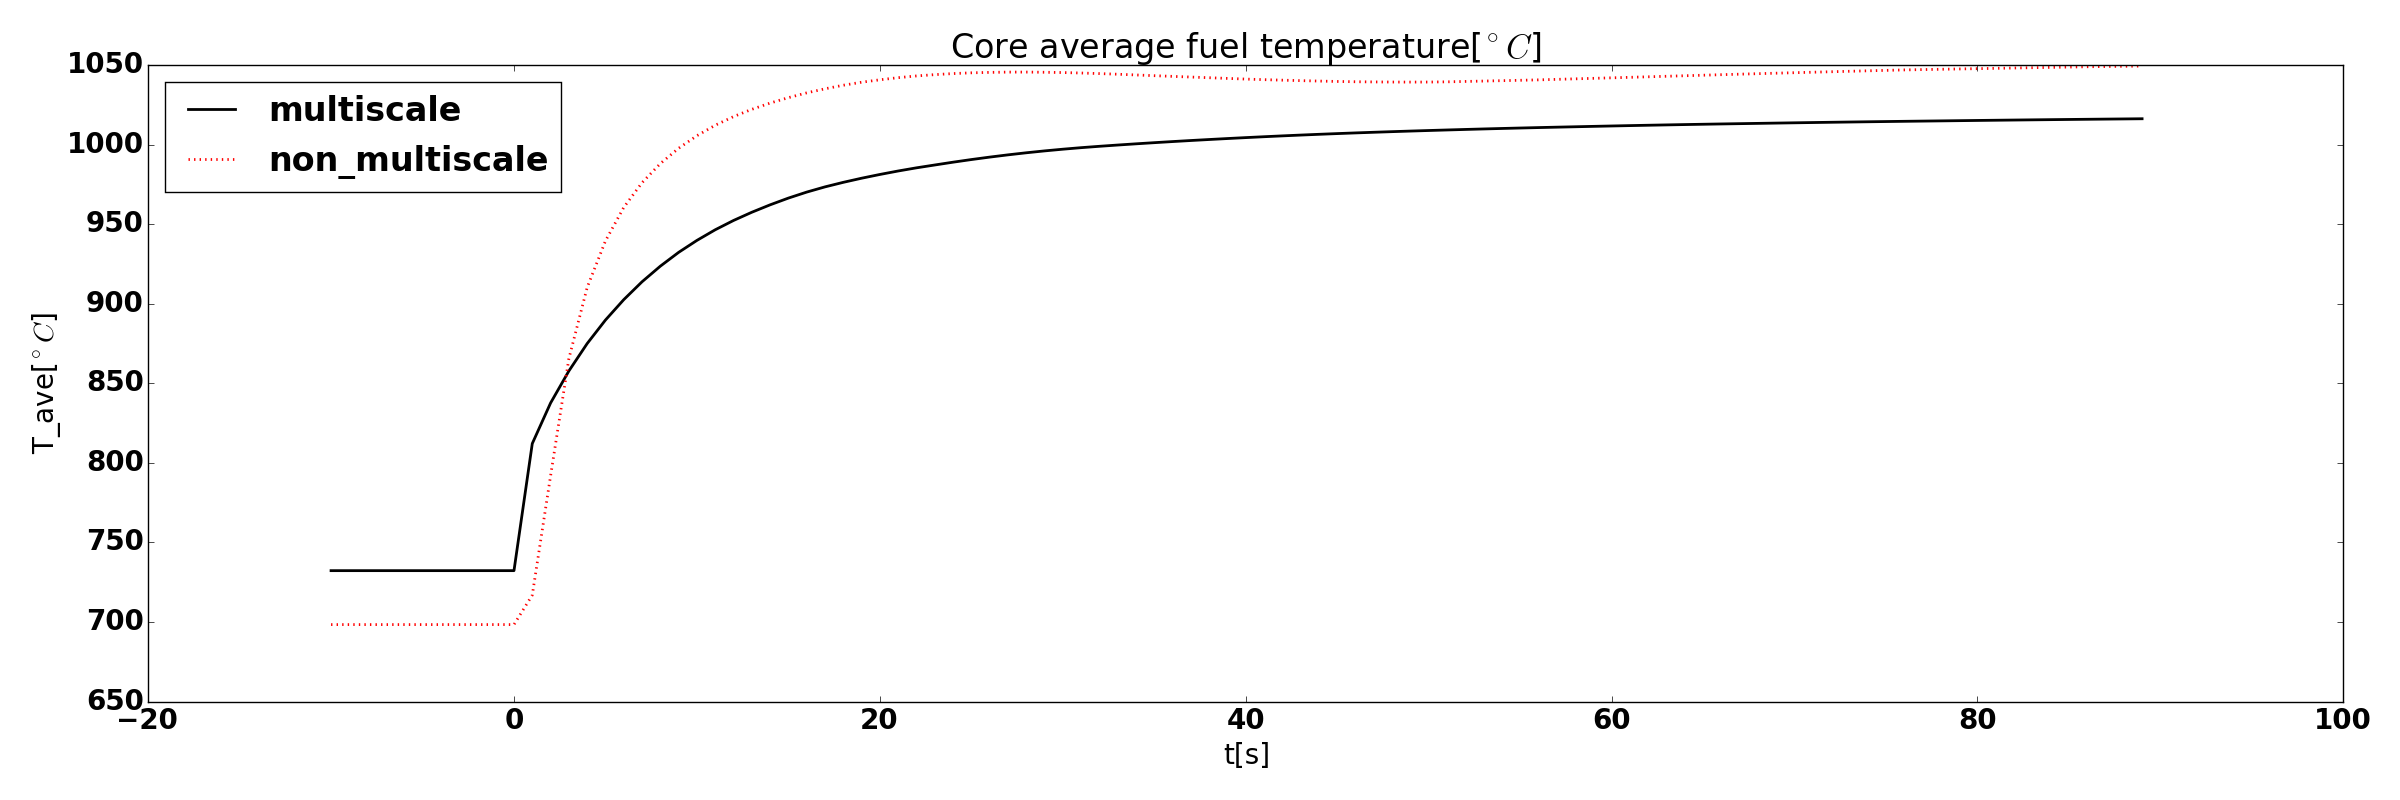
\includegraphics[width=\textwidth]{images/diffusion/tmsr/RI/compare_multiscale/T_fuel_ave.png}
    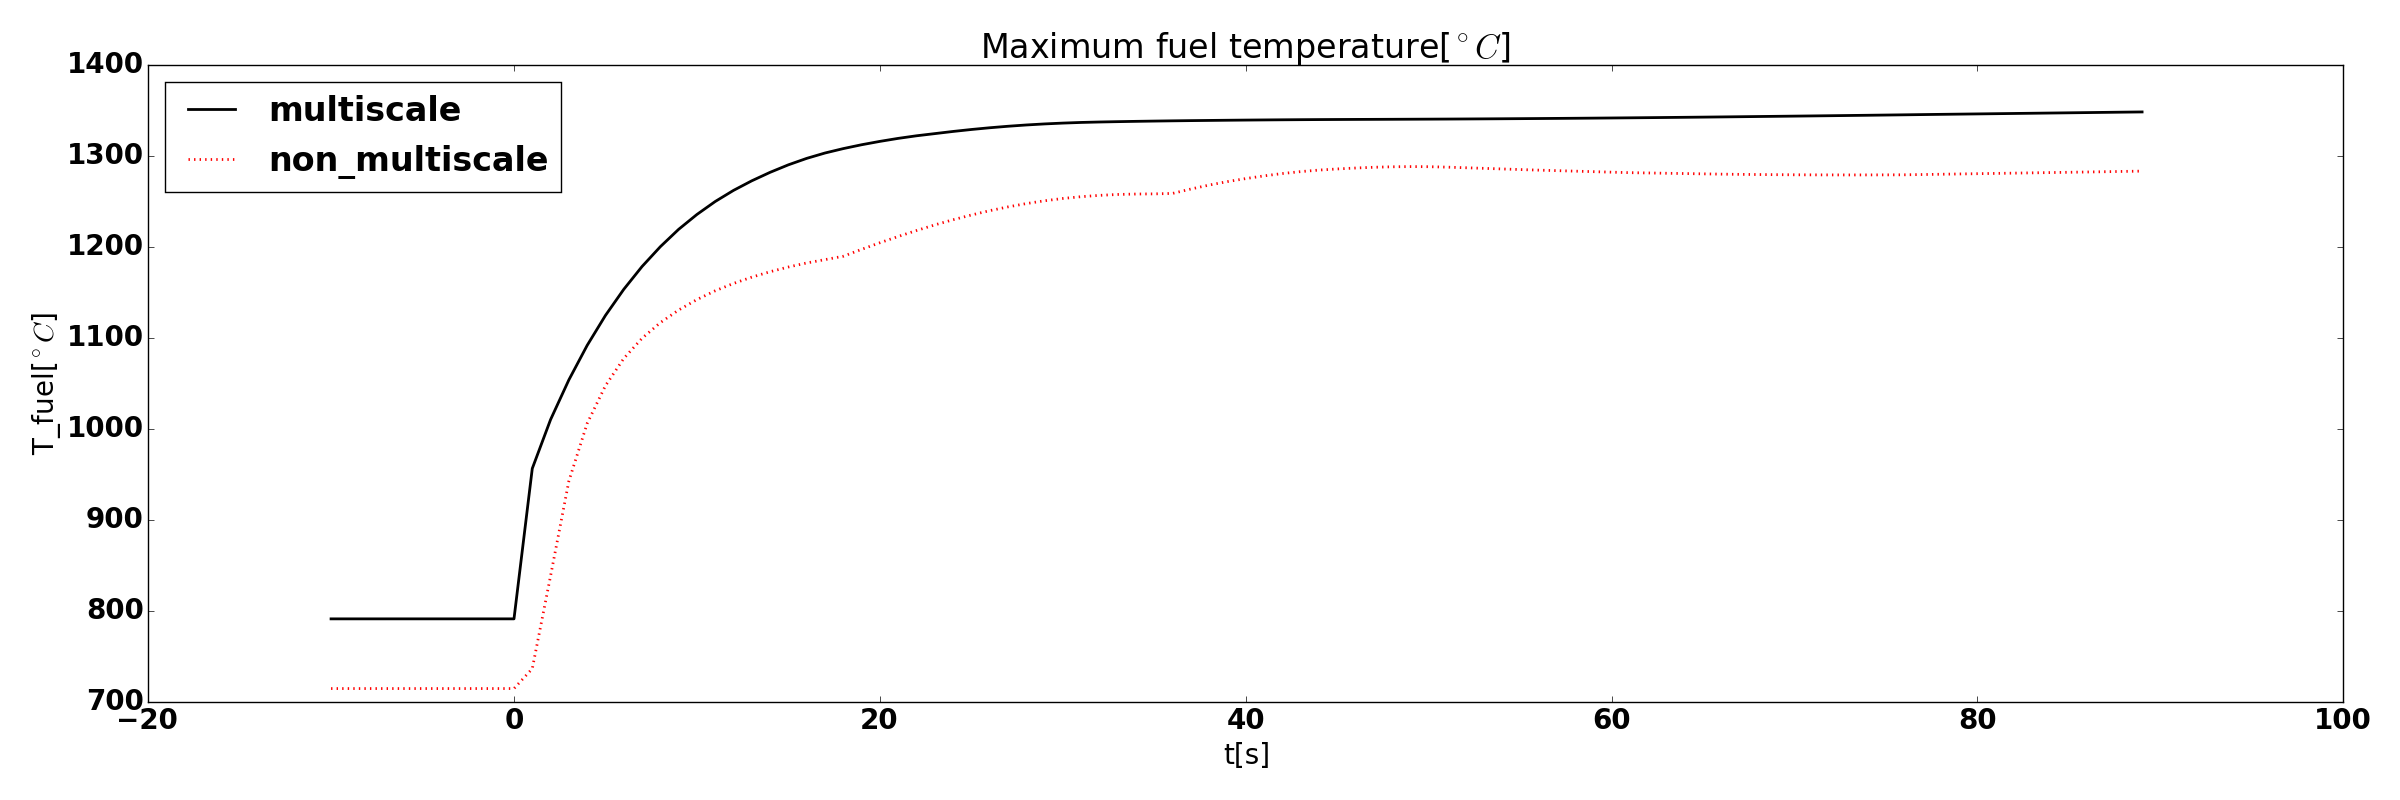
\includegraphics[width=\textwidth]{images/diffusion/tmsr/RI/compare_multiscale/T_fuel_max.png}
    \caption{Average and maximum fuel temperatures during a 1\$ reactivity insertion transient in TMSR SF-1, with or without multiscale treatment}
    \label{fig:multi_comp_fuel_TMSR}
\end{figure}

Starting from steady state under nominal conditions and with the same boundary conditions described in the previous section, 1\$ is inserted into the core at time 0. Although an insertion of 1\$ is highly unlikely due to the designed limit of the control rod, it is useful to test the model's ability to handle a large amount of reactivity insertion and to understand the core behaviour in this case as a bounding example. At the onset of the reactivity insertion transient, nuclear power rate increases due to excess of reactivity. Following the power excursion is the temperature rise in the core, first in the fuel, due to the direct deposit of the nuclear energy, and then in the coolant as the energy diffuses out of the fuel pebbles. By design, both elements provide negative temperature reactivity feedback that at the end re-stabilizes the core. 

Temperature reactivity feedback is the most important natural safety mechanism in the core during a reactivity insertion without SCRAM. In FHRs, the feedback from the Doppler broadening of the fuel resonance absorption cross-sections, i.e. the Doppler feedback, is much more prominent than the coolant void feedback. And it reacts promptly, because the Doppler feedback is directly initiated by the changes in the fuel temperature. As a result, the timescale of a reactivity insertion transient is short, shorter than the circulation time of the primary coolant, so the inlet coolant condition remains constant during the simulation.



Figure \ref{fig:multi_comp_power_TMSR} shows that the power excursion is less severe and the power stays at a lower level after the transient, when the detailed fuel temperature profile is used to compute the Doppler feedback. Also, the response is quicker in this case because the promptness of the Doppler feedback is properly captured. 


Comparison of the core average and maximum flibe temperatures between the conventional porous media model and the one with the multiscale treatment is shown in figure \ref{fig:multi_comp_flibe_TMSR}. 
The coolant flows upward through the fuel pebbles in the TMSR SF-1 core, so the hottest coolant is found at the top. In other words, the maximum coolant temperature also represents the outlet coolant temperature, one of the most important safety parameters in a FHR because this directly relates to the temperature of the metallic structures, the most vulnerable components in a FHR in terms of temperature safety margin.
The steady state flibe temperature is the same in both models, but both the average and the outlet coolant temperature rise to a higher value during the reactivity insertion transient in the non-multiscale case, the amount of heat deposited to coolant and the temperature reactivity feedback from the coolant are overestimated. 

Figure \ref{fig:multi_comp_fuel_TMSR} shows the average and maximum fuel temperature in the core during the transient, obtained with or without the mutliscale treatment. 
The peak fuel temperature in the multiscale case is higher at steady state, because the inner layers with higher temperatures are included in the average, and it remains higher during the reactivity insertion transient because of the spread in temperature inside fuel elements. On the other hand, although the average fuel temperature in the multiscale case is higher at steady state due to the higher temperatures inside the fuel elements, it is lower at the end of the transient because the reactor core stabilize at a lower power than the non multiscale case. In general, the peak fuel temperature, from which the safety margin to fuel damage is computed, is a more important safety parameter for the fuel. The conventional porous media model underestimates the peak fuel temperature during a reactivity insertion transient and could lead to an overly optimistic safety margin with respect to fuel damage during reactivity insertion transients. 

Overall, the conventional model overestimates the temperature increase in the coolant and in the average fuel temperature, whereas it underestimates the peak fuel temperature. However, when comparing the results, we need to keep in mind of the uncertainties introduced by the material properties used in both approach. In fact, pebble wise average properties are used in the non-multiscale case, whereas more detailed layer wise properties are used in the multiscale case, and large uncertainties are associated with the measurement of all these values. A large variation exists in the limited literature on TRISO fuel pebble thermal properties measurements. In addition, to simplify the computation, the outer non-power-generating layers in TRISO particles are combined into one, with an equivalent conductivity computed from the properties of the substituting materials. 
The contact resistance at the interfaces of the layers are not taken into account when computing the equivalent properties because of lack of available measurements. 

To evaluate the sensitivity of the results to the material properties, in particular thermal conductivity values of the fuel elements, figure \ref{fig:temps_TMSR} shows the core average temperatures in each TRISO and pebble layer during the 1\$ reactivity insertion transient, with either nominal material properties (table \ref{tab:triso_prop_tmsr1} and table \ref{tab:pb_prop_tmsr1}) or an uniform thermal conductivity (193 W/m.K, a typical value for nuclear graphite material) for each layer. 
In each individual TRISO particle, the center is the hottest and the temperature decreases as the heat diffuses out of the fuel material. With the nominal properties, a large temperature drop occurs at the coating due to the buffer layer. The buffer layer in a TRISO particle has a porous structure that serves as a damper to the stress caused by gaseous fission production. The porous nature of this layer makes it a thermal insulator and sets the lower bound of the conductivity. The buffer layer has the most temperature variation compare to the other layers.
In both cases, the temperatures deviate further from each other during the transient, because of the elevated power level. And the temperatures are further apart with the nominal thermal conductivity values.   

\begin{figure}
    \centering
    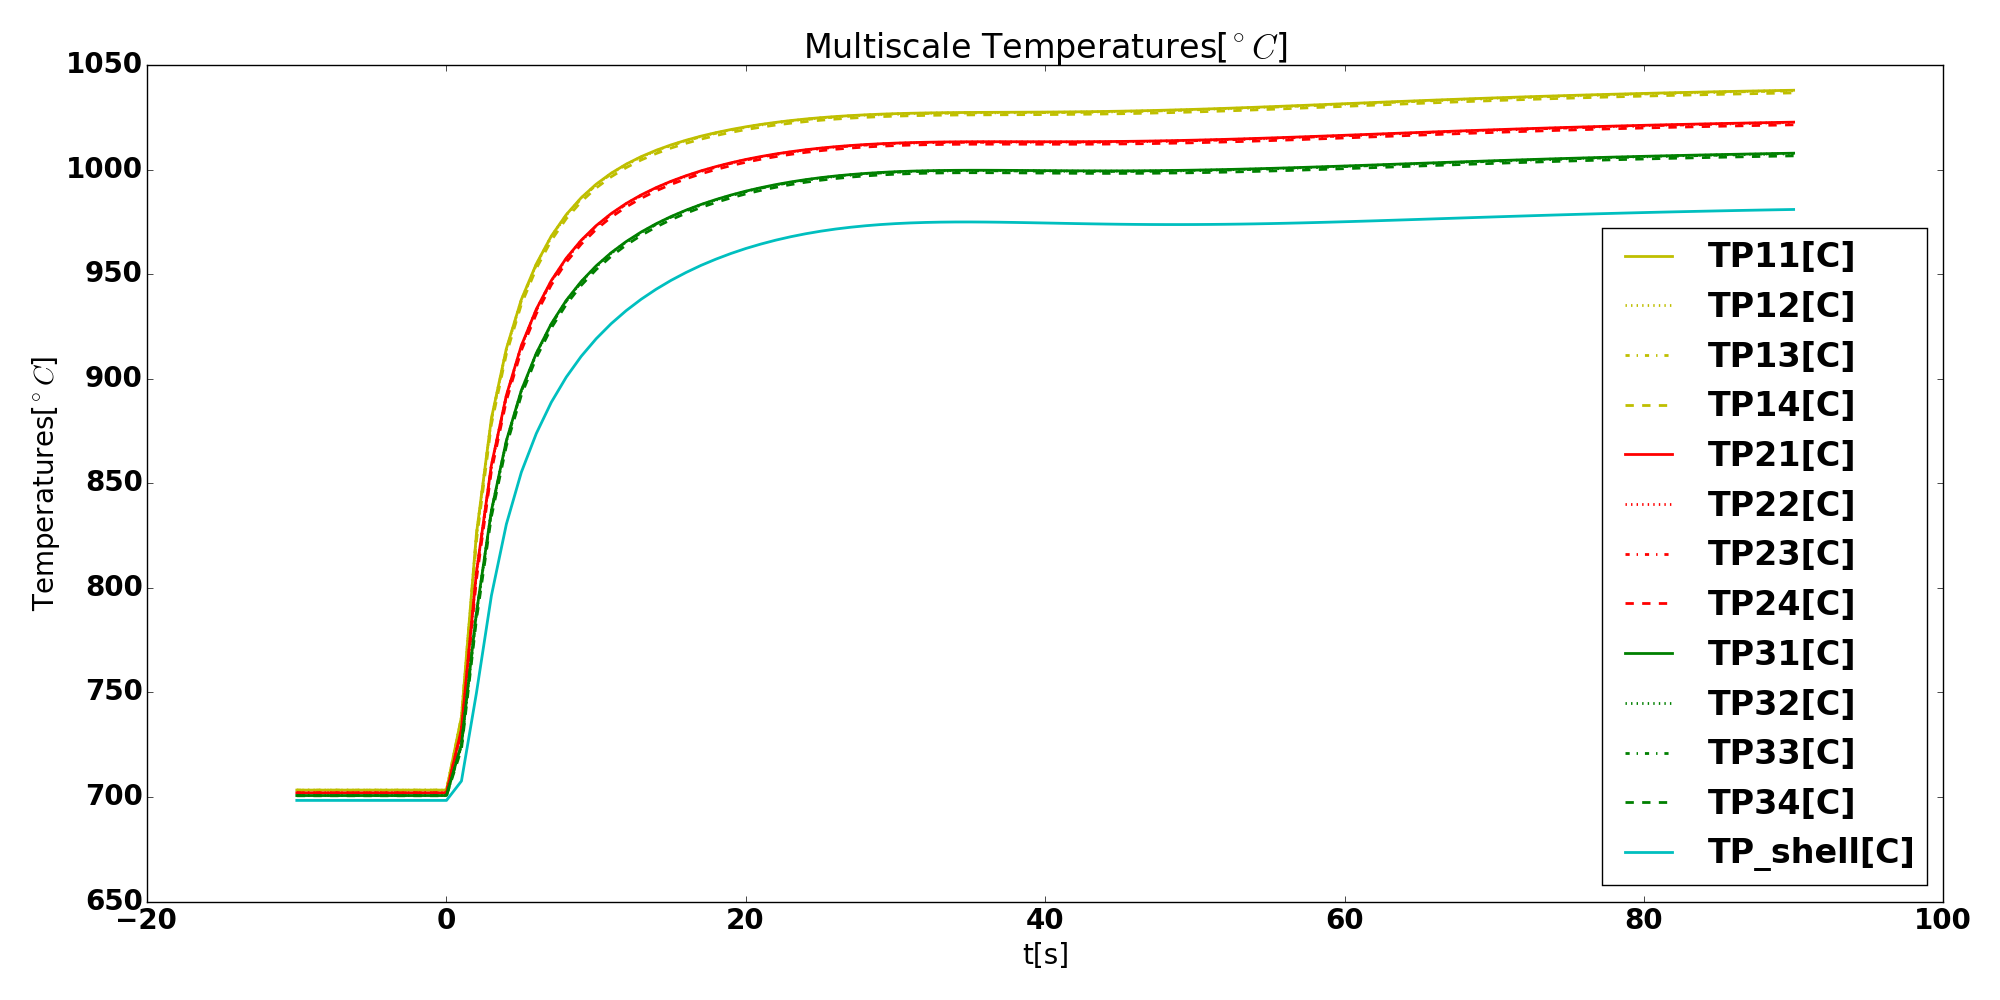
\includegraphics[width=\textwidth]{images/diffusion/tmsr/RI/compare_multiscale/temps_large_k.png}
    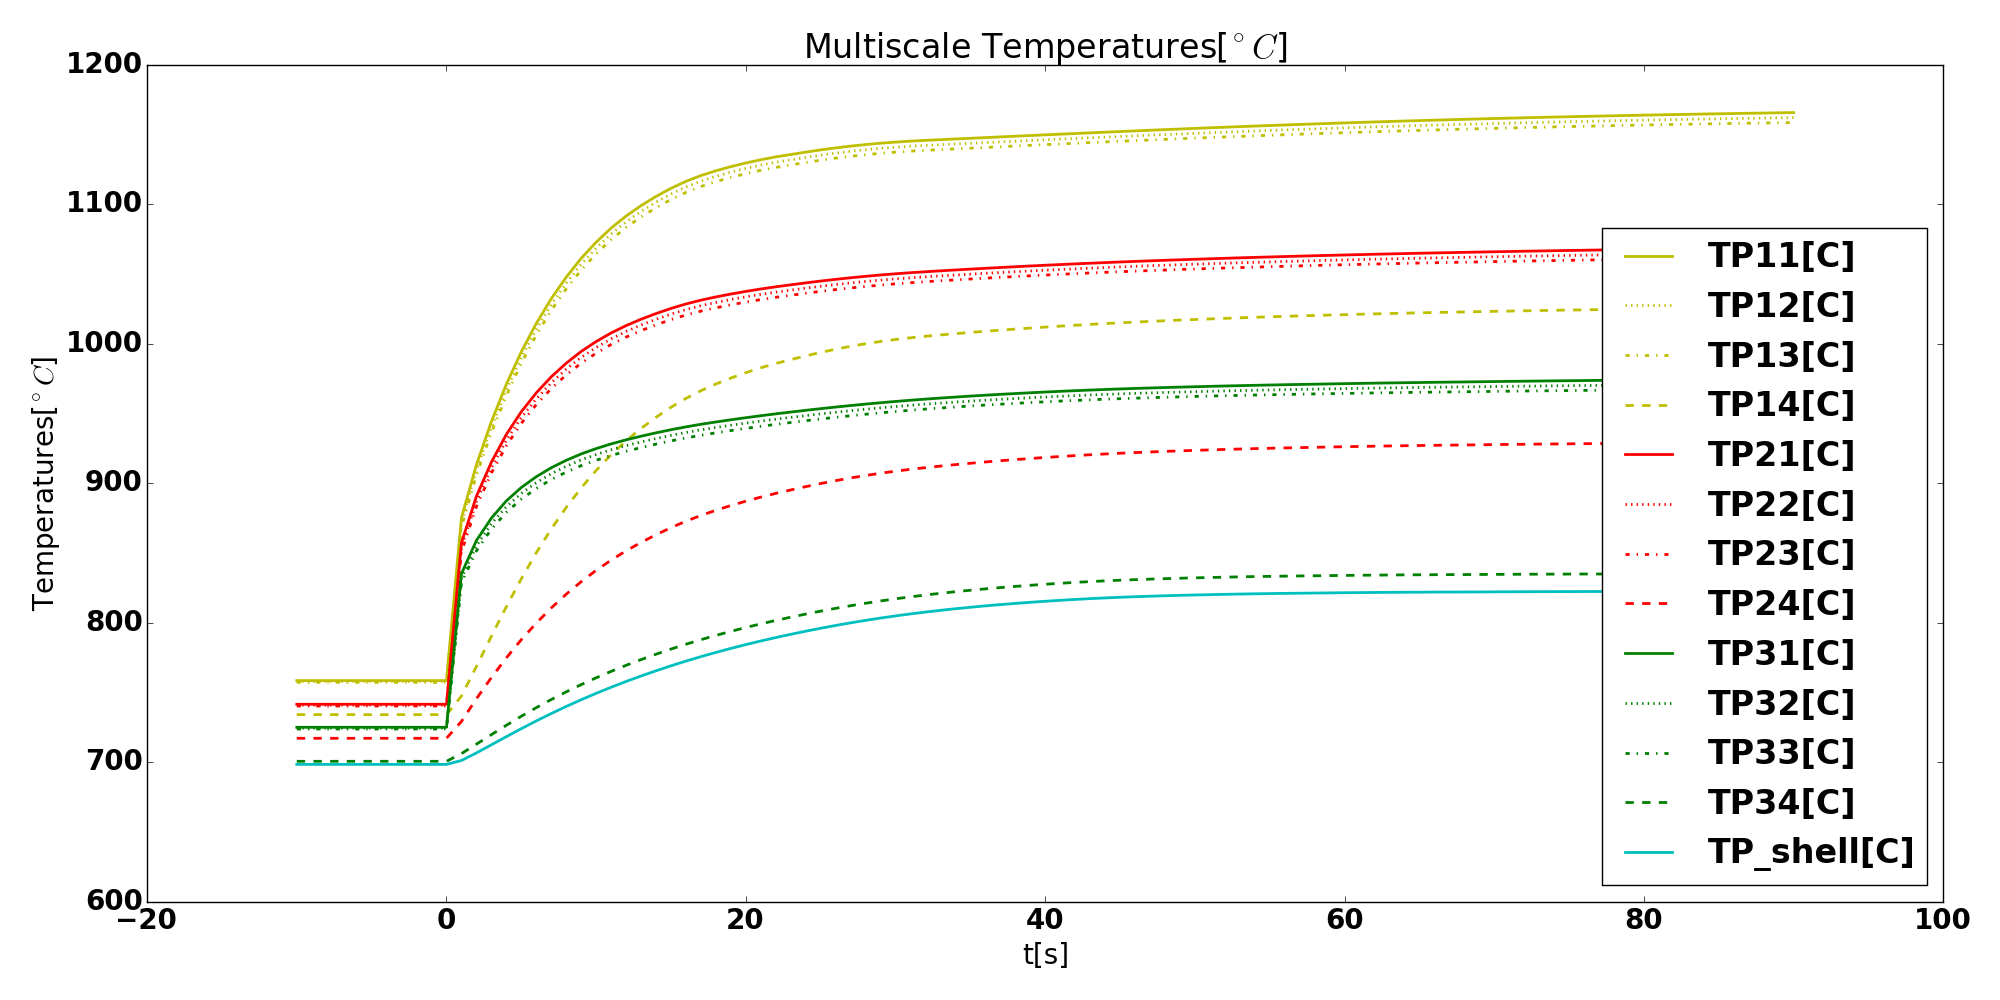
\includegraphics[width=\textwidth]{images/diffusion/tmsr/RI/compare_multiscale/temps_nominal_k.png}
    \caption{Core average temperature inside fuel elements during 1\$ reactivity insertion transient for TMSR SF-1, with a large thermal conductivity posed to all material(top) or with nominal material properties for each layer(bottom). Notation for temperatures: $TP_{ij}$ represents the jth TRISO layer in the ith pebble layer. (A fuel core in a pebble is divided into three layers and within each layer, a TRISO particle is divided into four layers - three fuel layers and one coating layer.). And $TP_{shelll}$ is the temperature in the graphite shell of the pebble.} 
    \label{fig:temps_TMSR}
\end{figure}

 
\newpage
As discussed before, the multiscale treatment is important in capturing the correct feedback behaviour, so the results shown hereafter are with the treatment.  
Figure \ref{fig:RI_pcm} shows the power and temperature evolution during a 1\$ or 0.5\$ reactivity insertion. 
 During the 1\$ prompt insertion transient, the core maximum fuel temperature is 1500$^{\circ}C$, below the safety limit(1600$^{\circ}C$). 
Coolant temperature is raised by only 100$^{\circ}C$ at the peak. 


\begin{figure}[h]
    \centering
        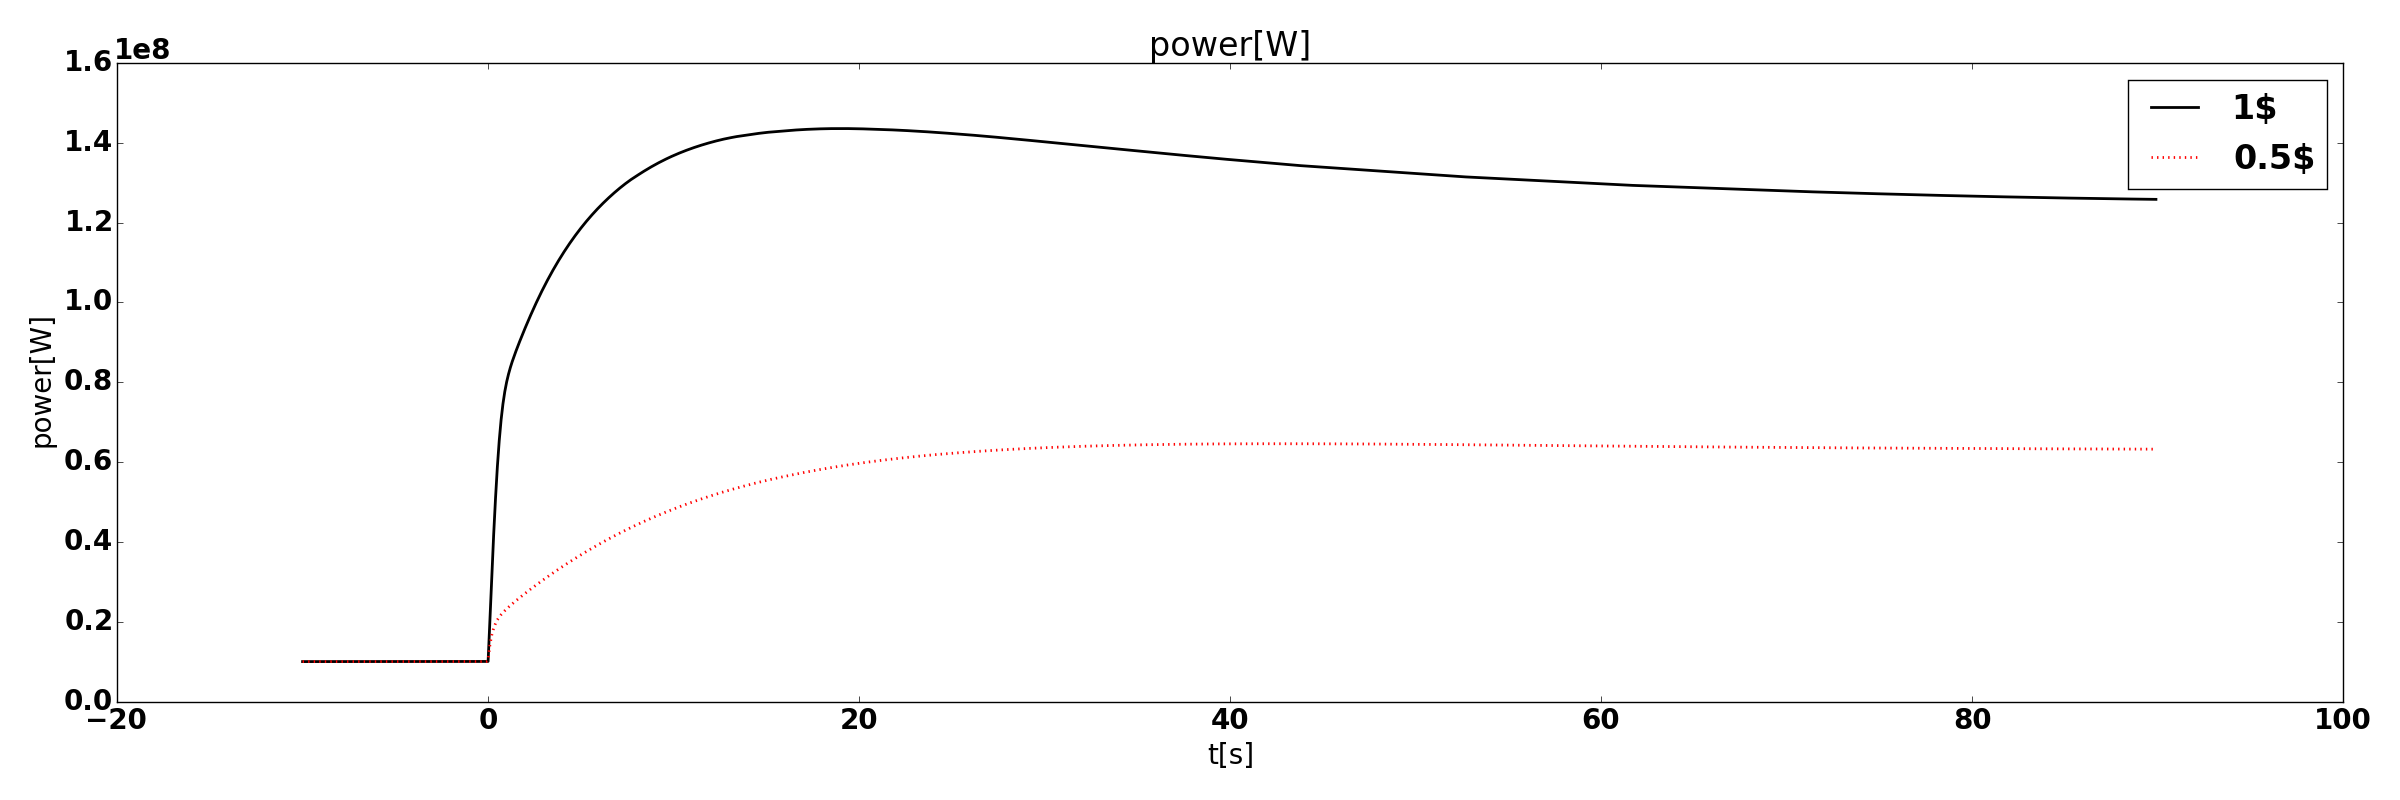
\includegraphics[width=1\linewidth]{./images/diffusion/tmsr/RI/diff_pcm/power.png}
        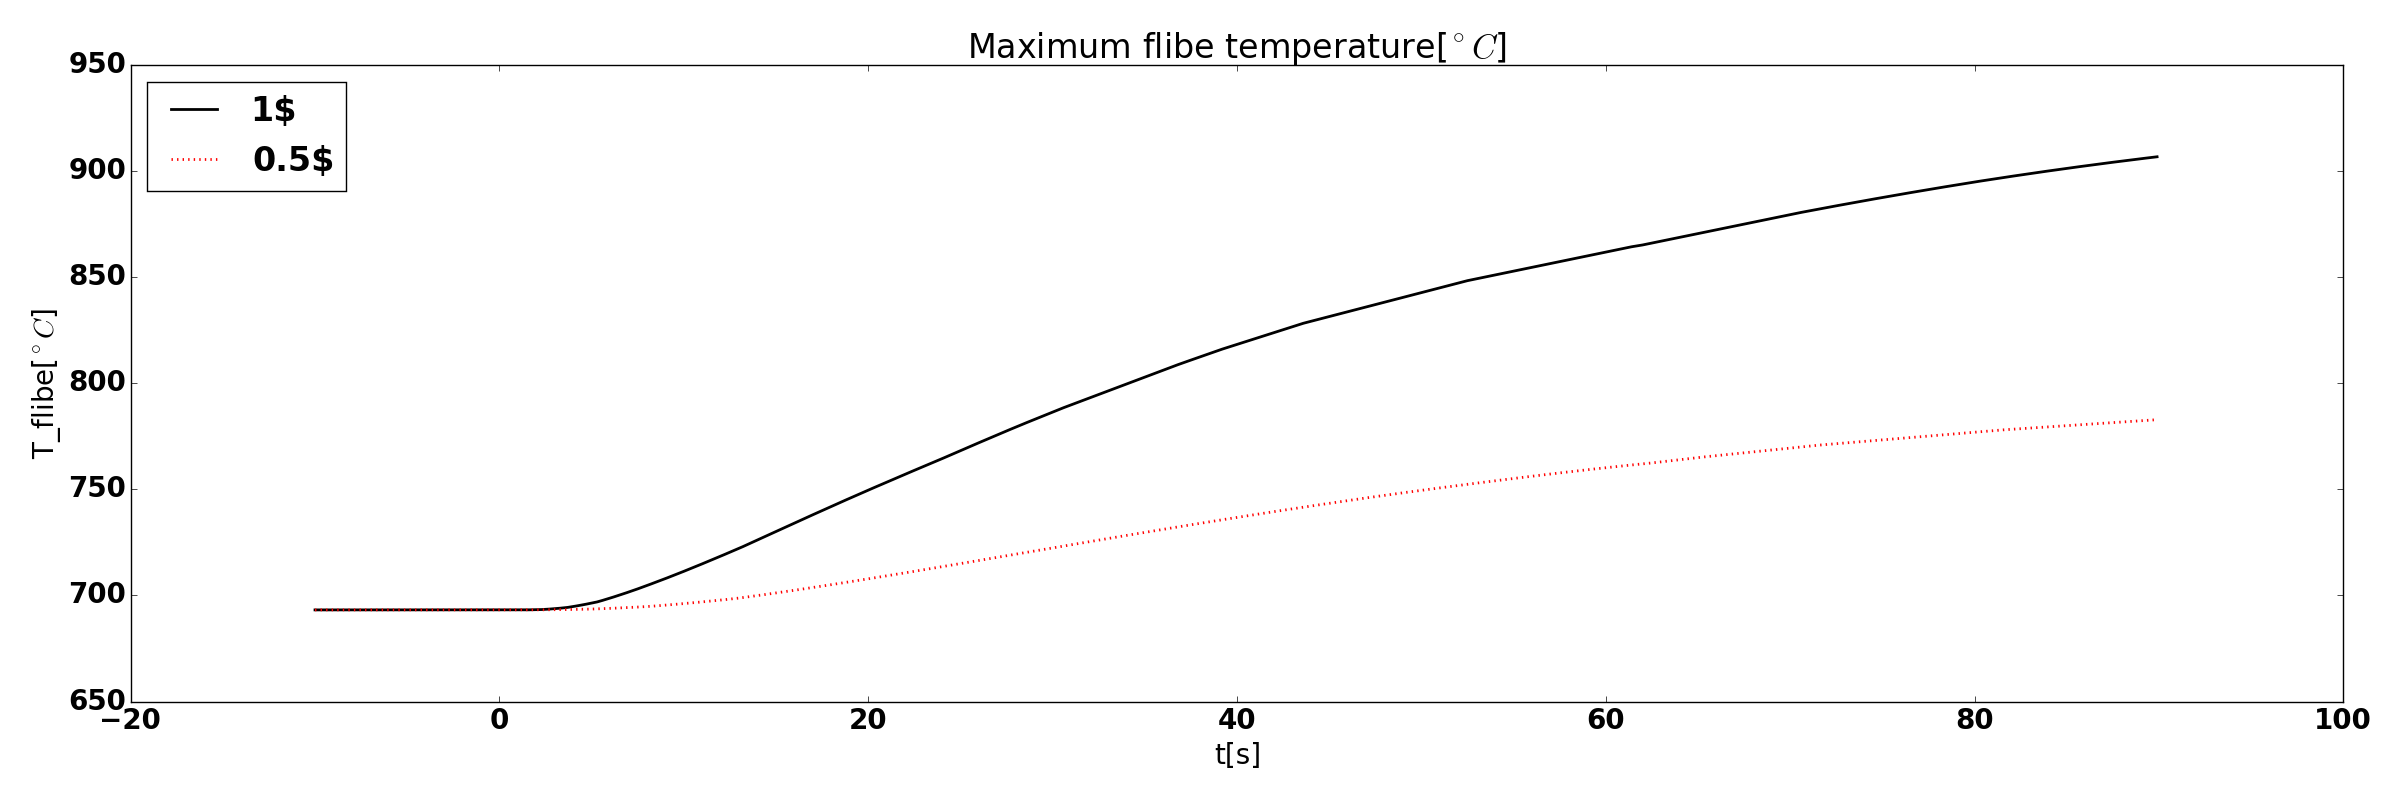
\includegraphics[width=1\textwidth]{./images/diffusion/tmsr/RI/diff_pcm/T_flibe_max.png}
        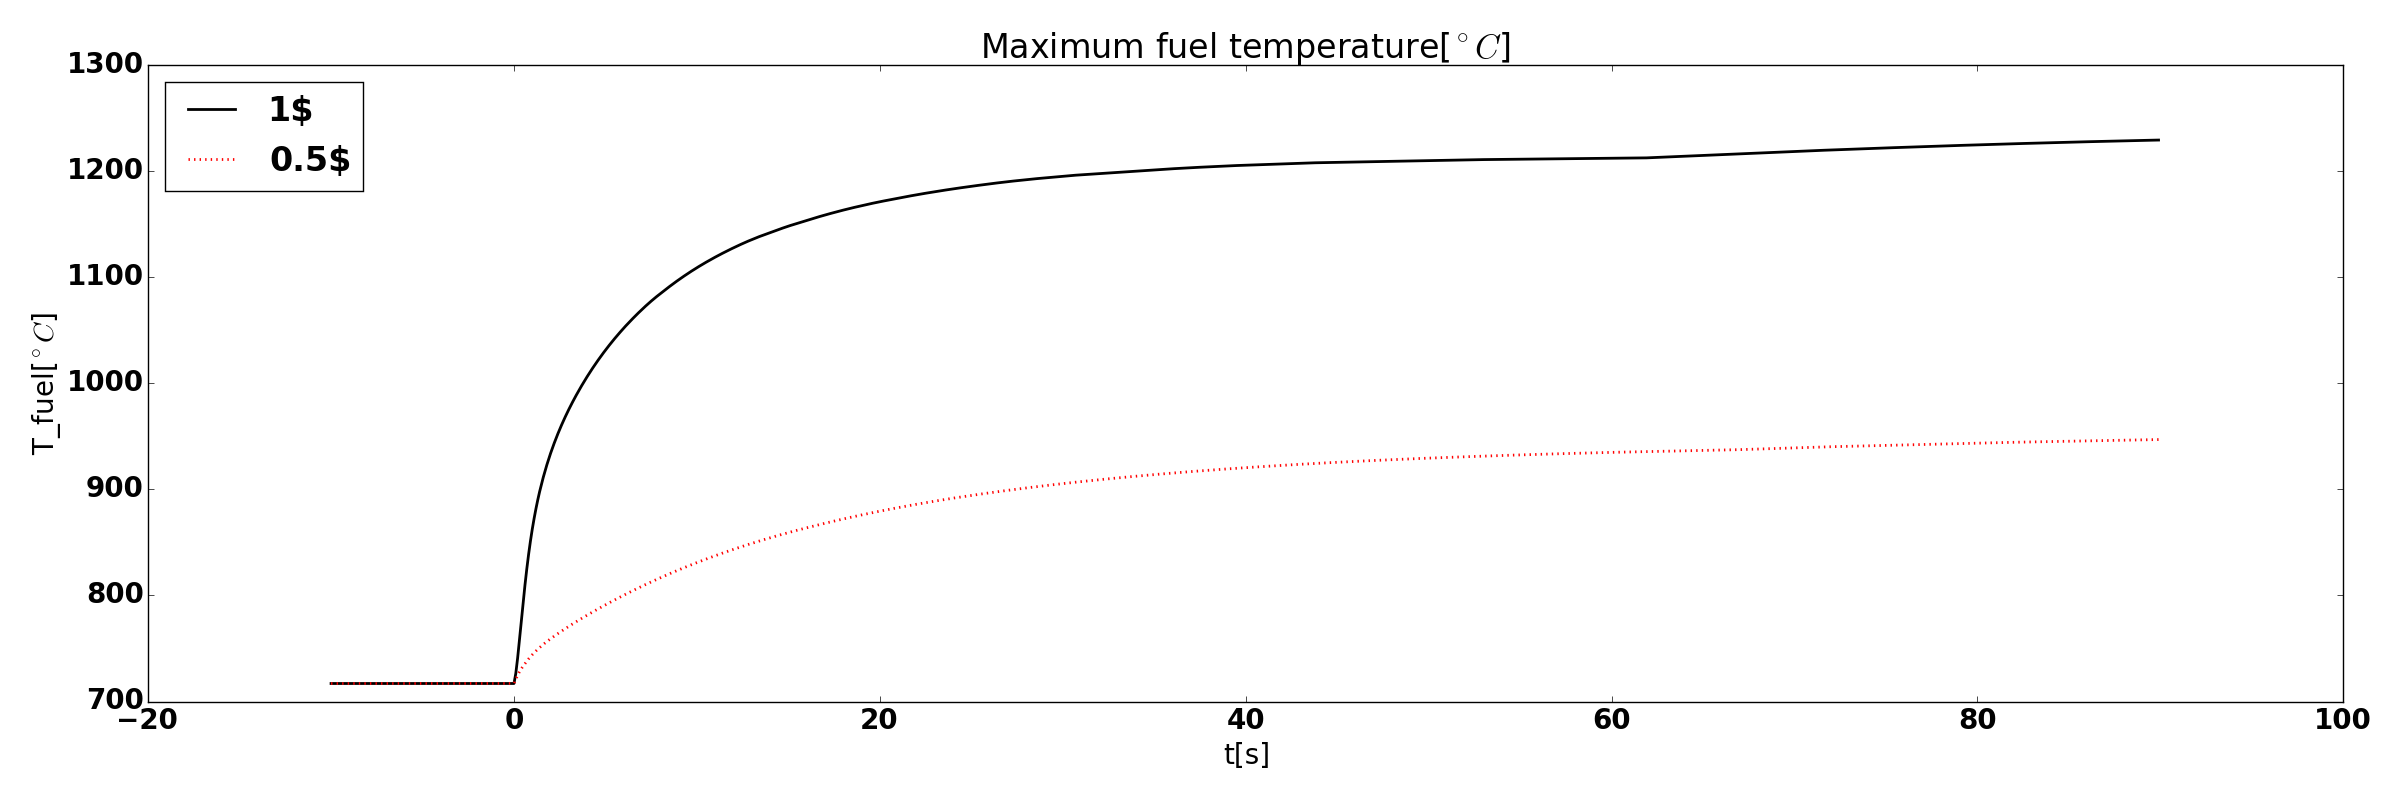
\includegraphics[width=1\textwidth]{./images/diffusion/tmsr/RI/diff_pcm/T_fuel_max.png}
    \caption{RI transients results}
    \label{fig:RI_pcm}
\end{figure}


Figure \ref{fig:RI_time} shows the effect of the timescale of the reactivity insertion on the safety parameters. Without SCRAM, the reactor reaches the same end state due to reactivity feedback mechanisms. However, safety measures can take in place to mitigate the consequence if the transient is slow. 

\begin{figure}[h]
    \centering
        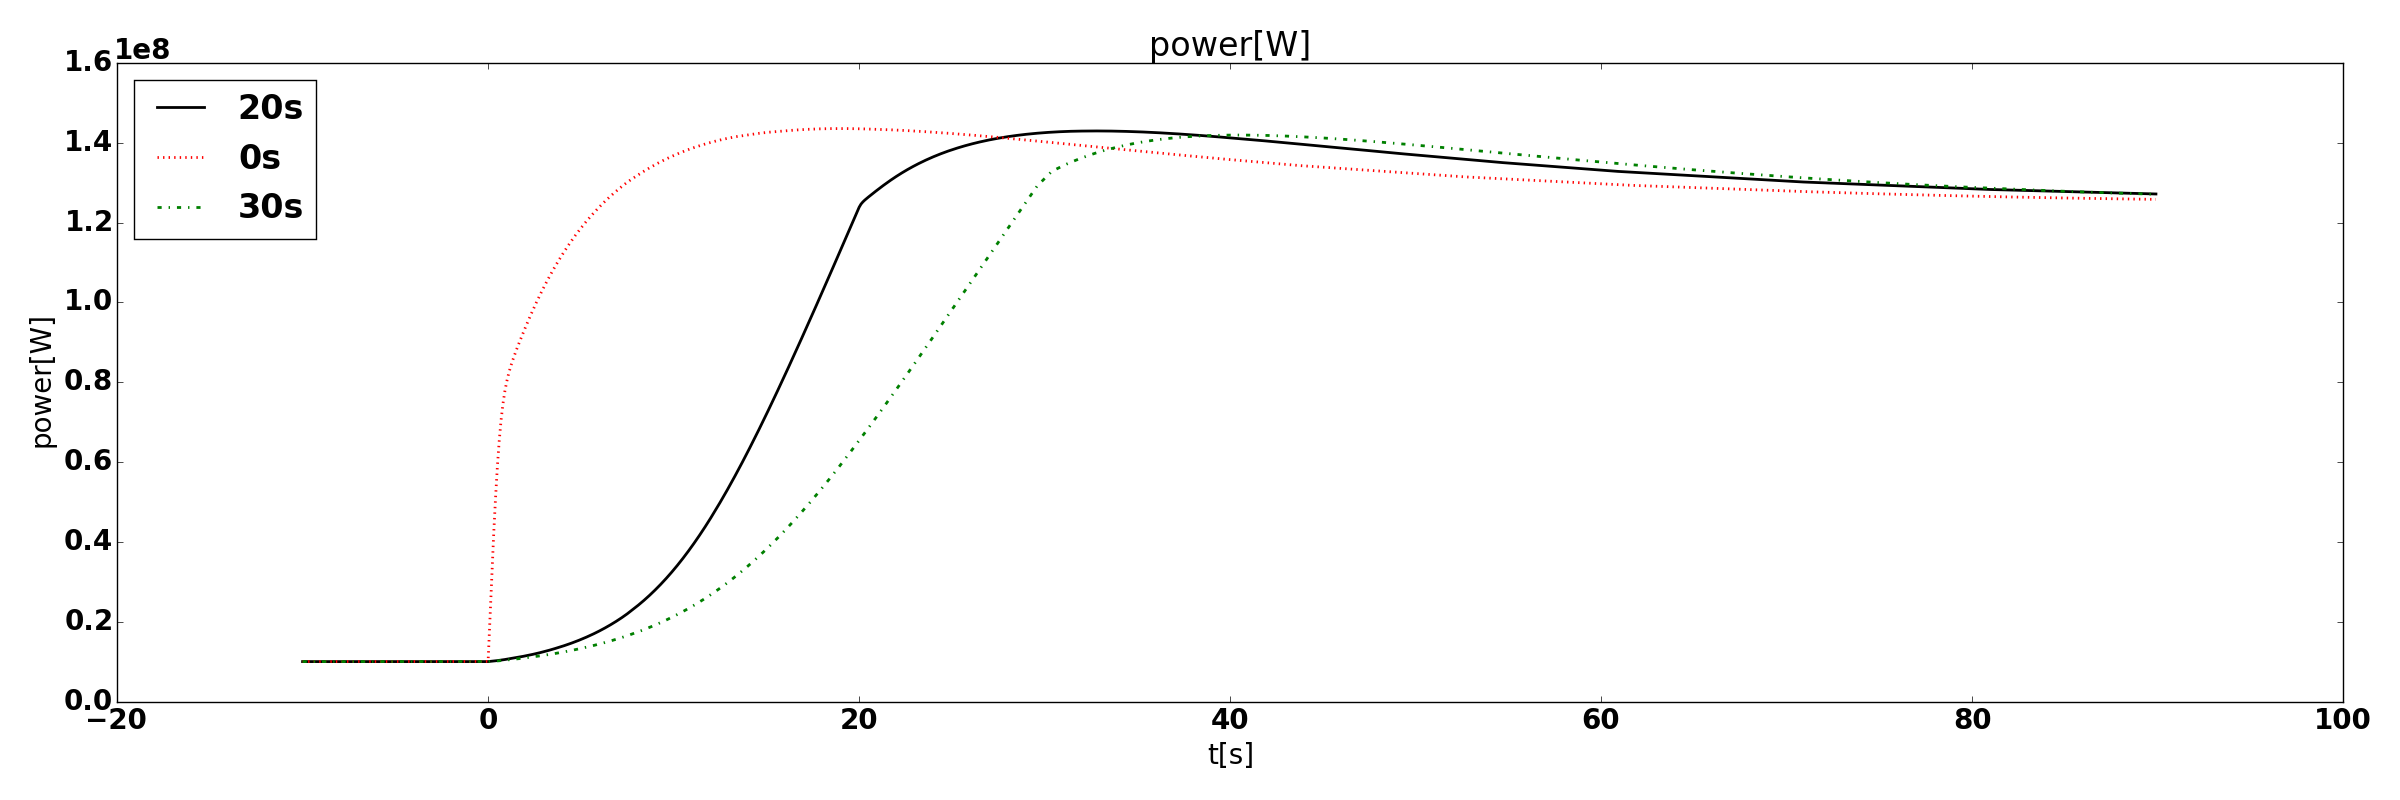
\includegraphics[width=\textwidth]{./images/diffusion/tmsr/RI/diff_time/power.png}
        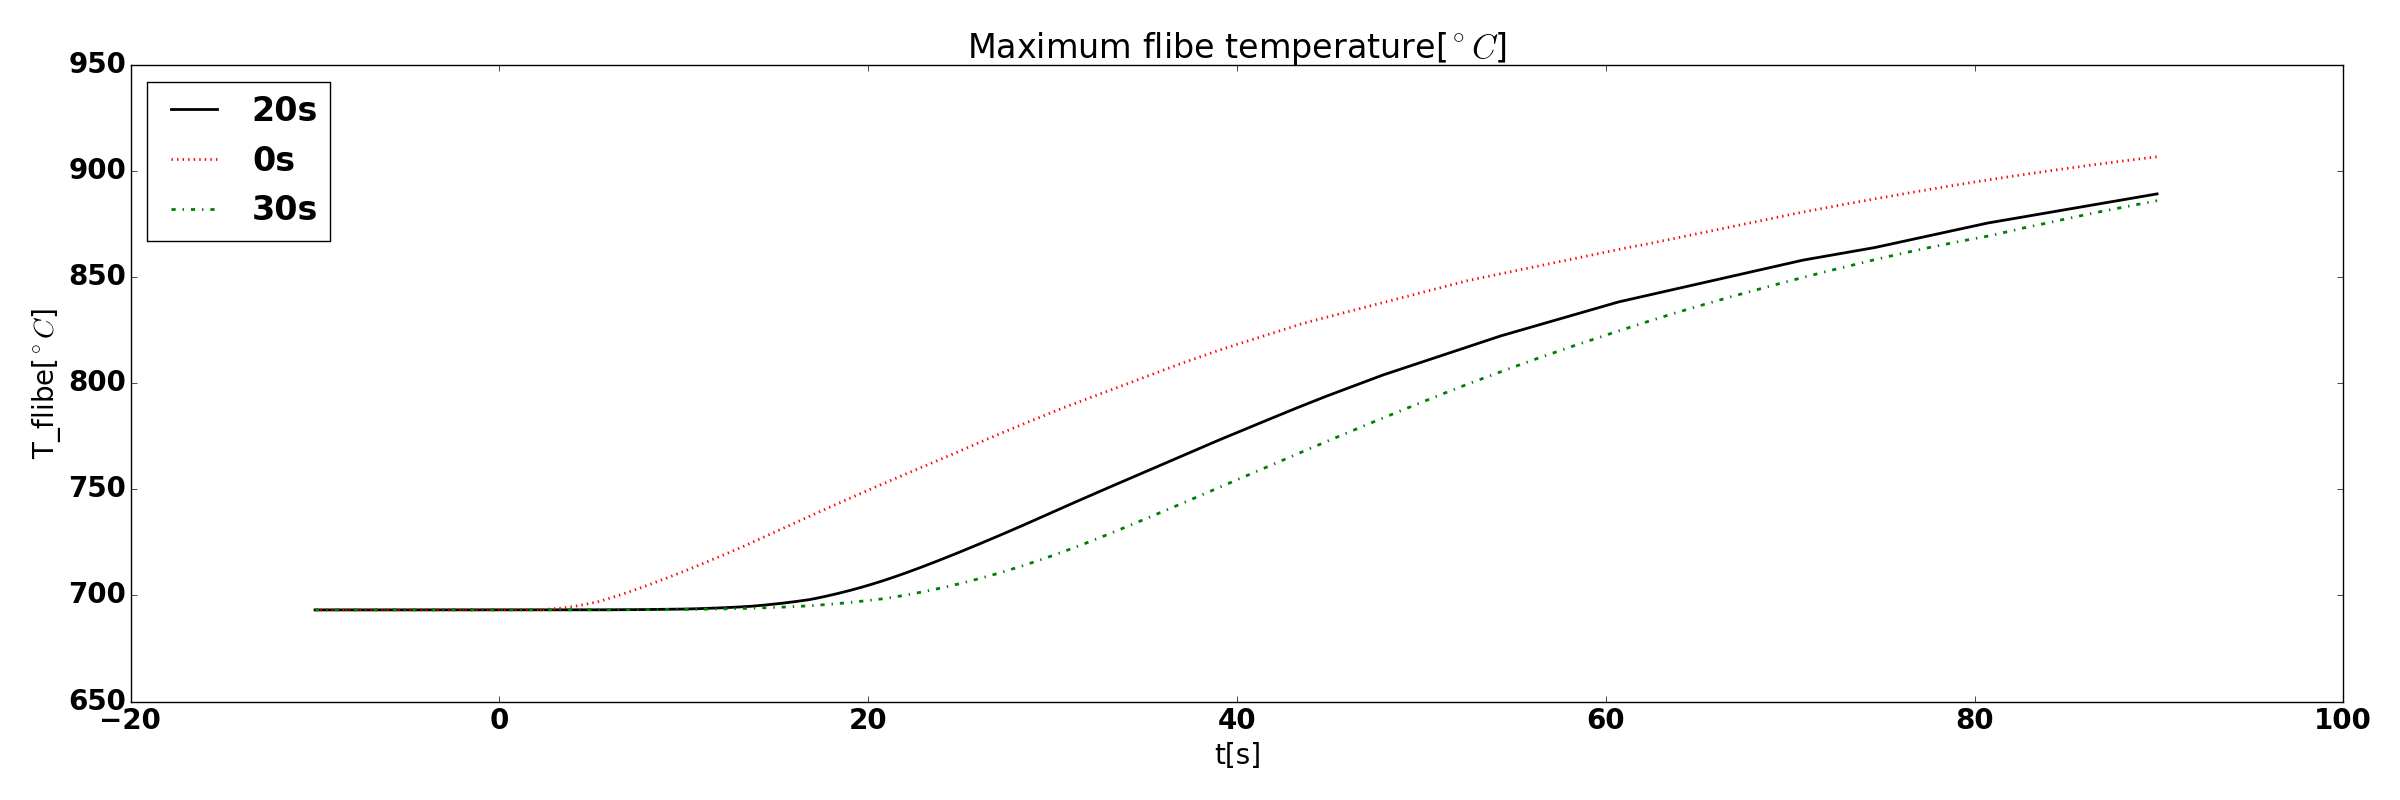
\includegraphics[width=\textwidth]{./images/diffusion/tmsr/RI/diff_time/T_flibe_max.png}
        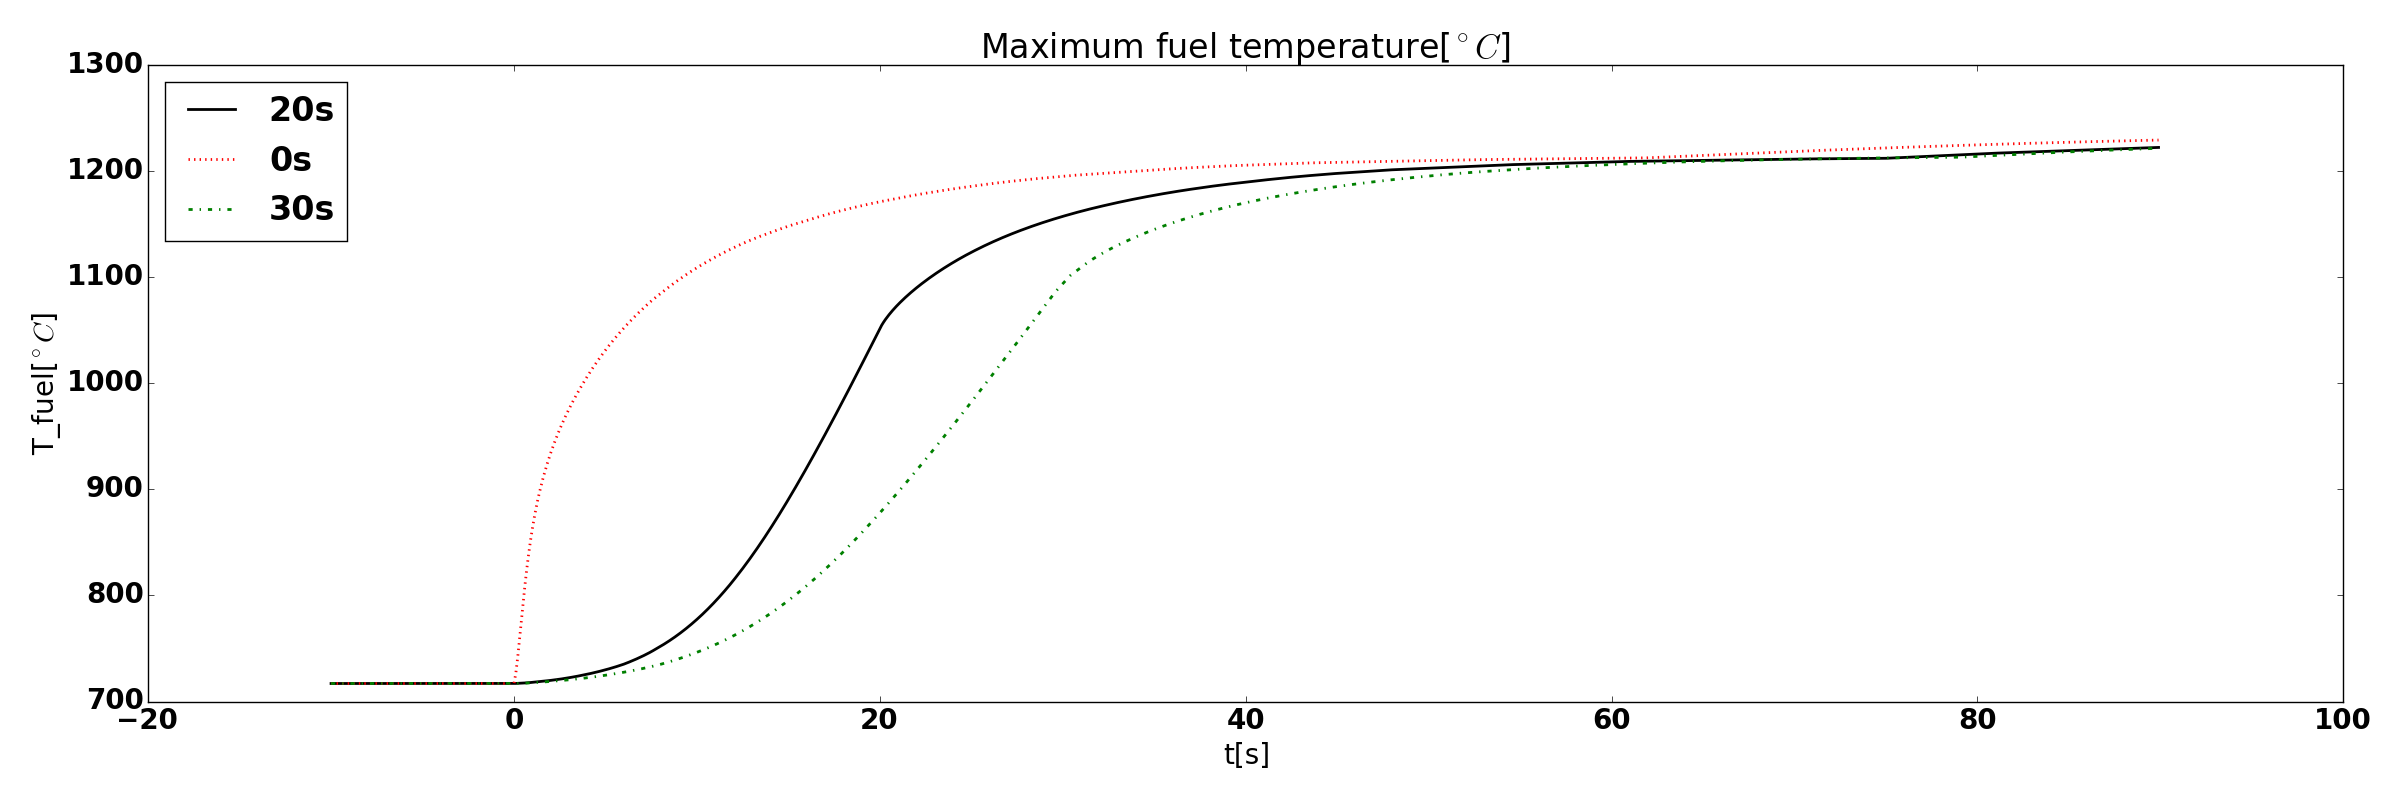
\includegraphics[width=\textwidth]{./images/diffusion/tmsr/RI/diff_time/T_fuel_max.png}
    \caption{RI transients results}
    \label{fig:RI_time}
\end{figure}




\newpage
\subsection{Overcooling transients}

\begin{figure}[h]
    \centering
        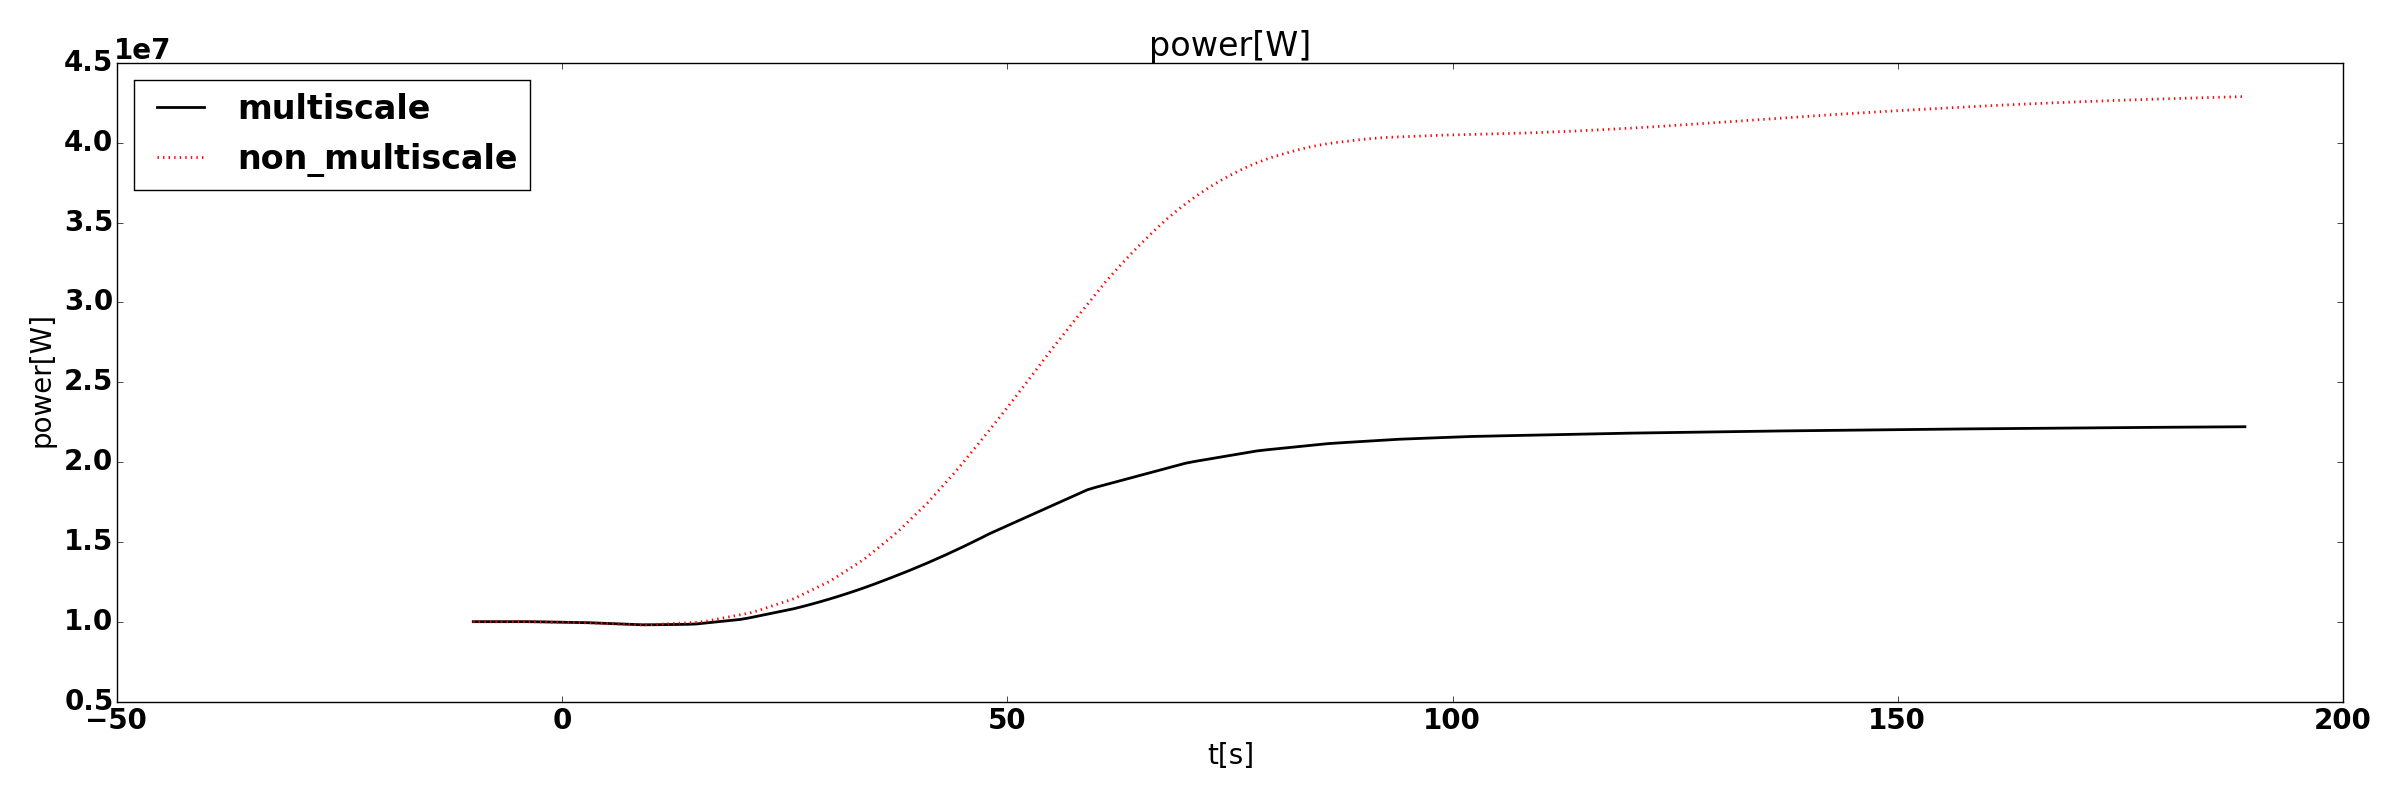
\includegraphics[width=1\linewidth]{./images/diffusion/tmsr/OC/compare_multiscale/power.png}
        \caption{Full core power during overcooling transient}
        \label{fig:OC_power}
\end{figure}


\begin{figure}[h]
    \centering
        
        \centering
        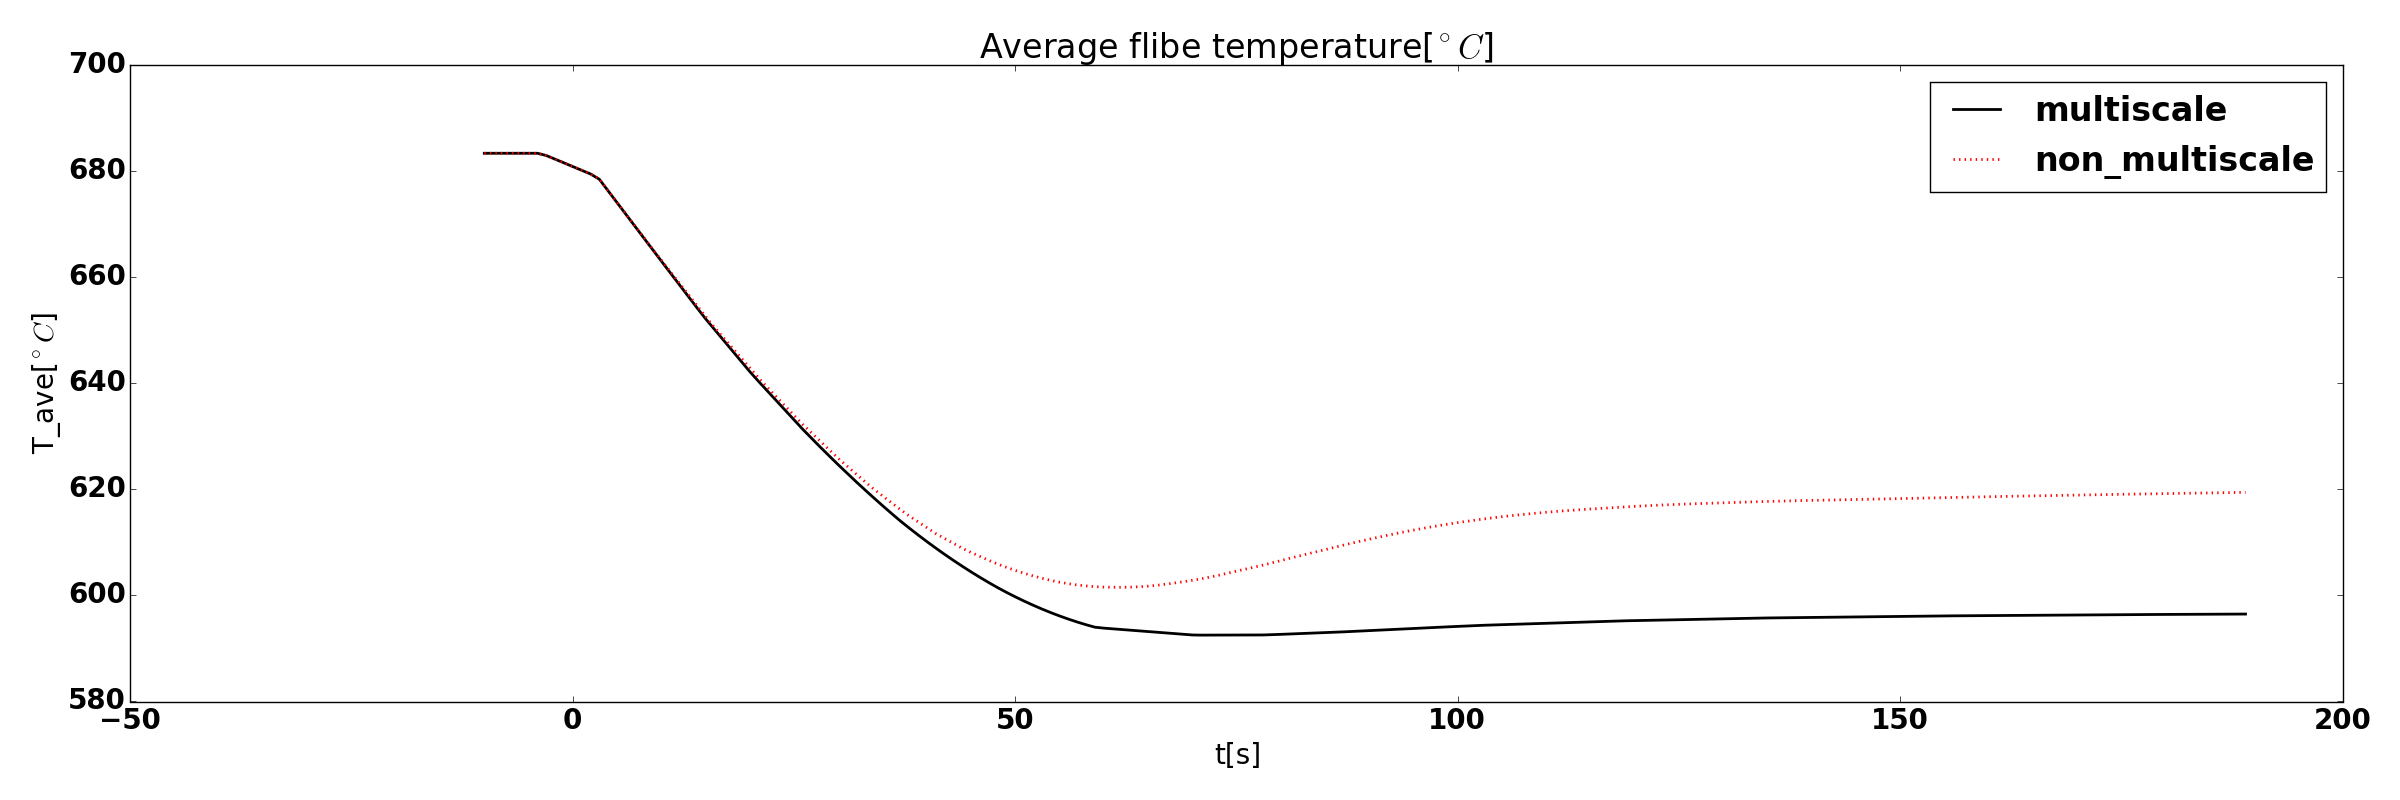
\includegraphics[width=1\textwidth]{./images/diffusion/tmsr/OC/compare_multiscale/T_flibe_ave.png}
        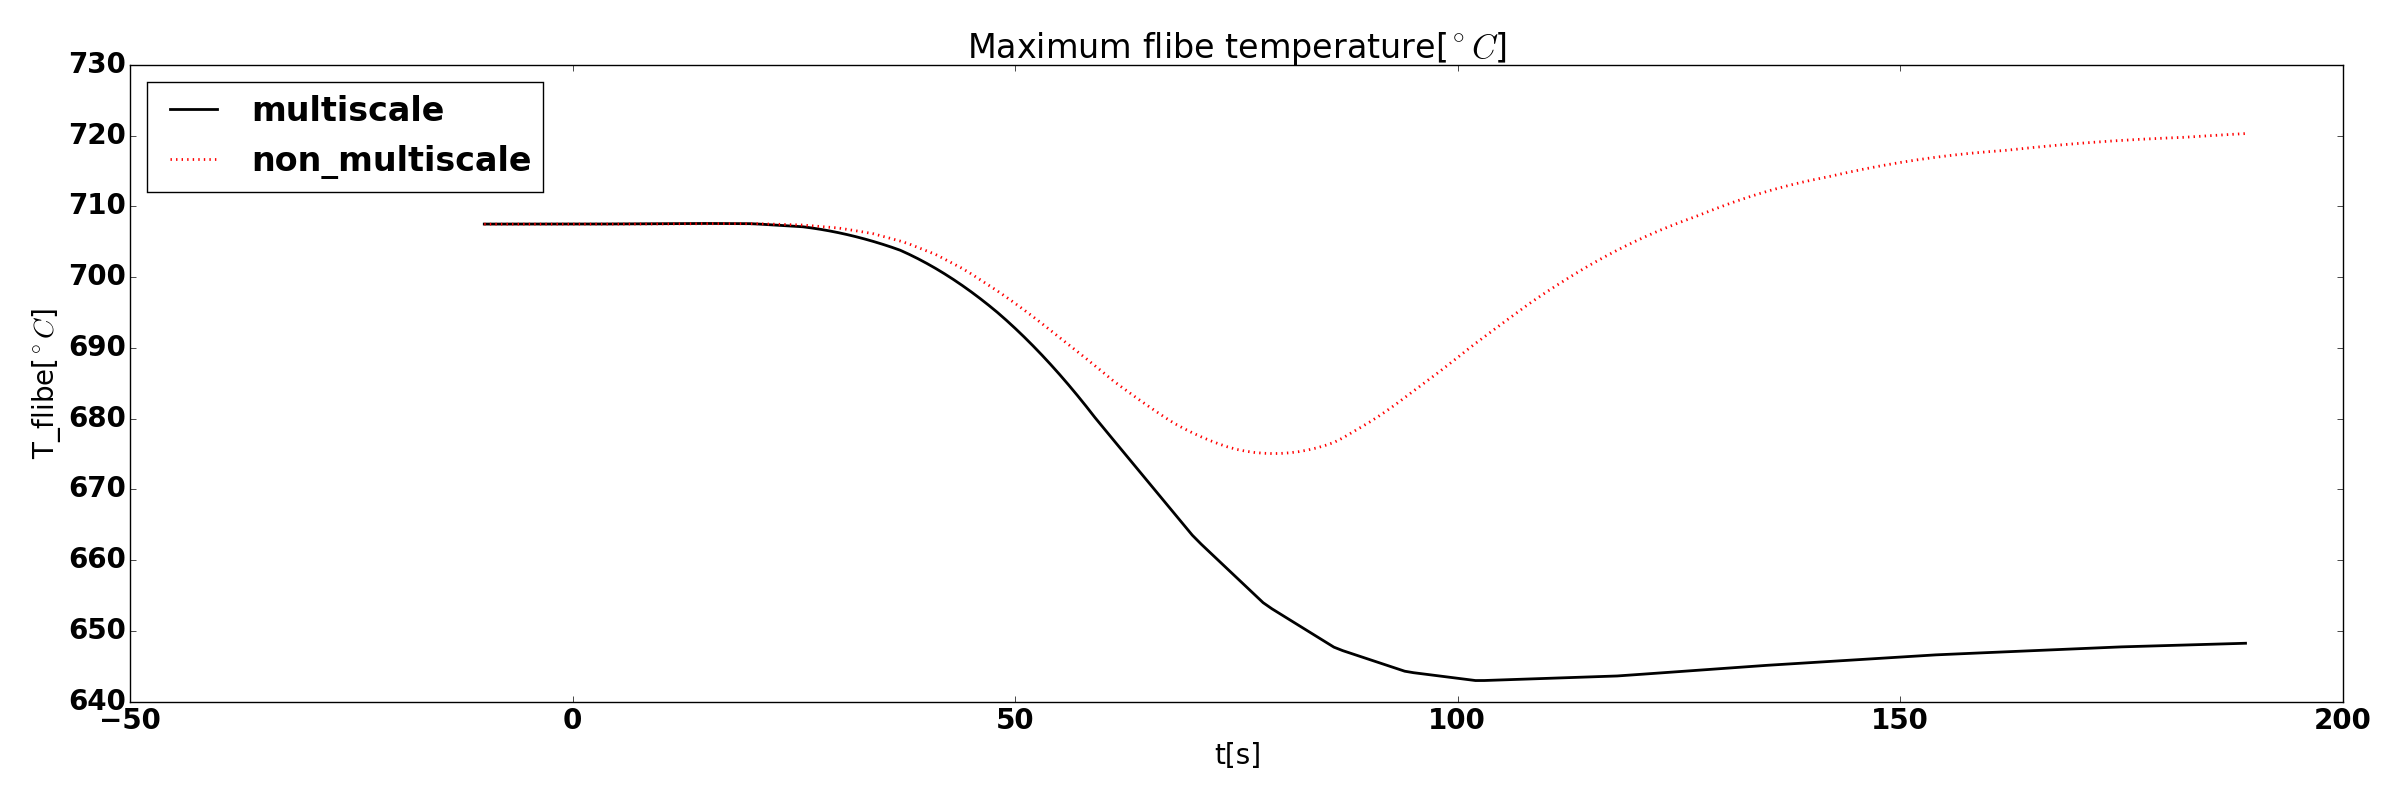
\includegraphics[width=1\textwidth]{./images/diffusion/tmsr/OC/compare_multiscale/T_flibe_max.png}
        \caption{Core maximum and average flibe temperature during overcooling transient}
        \label{fig:tmsr_oc_flibe}
\end{figure}


\begin{figure}[h]
    \centering
        
        \centering
        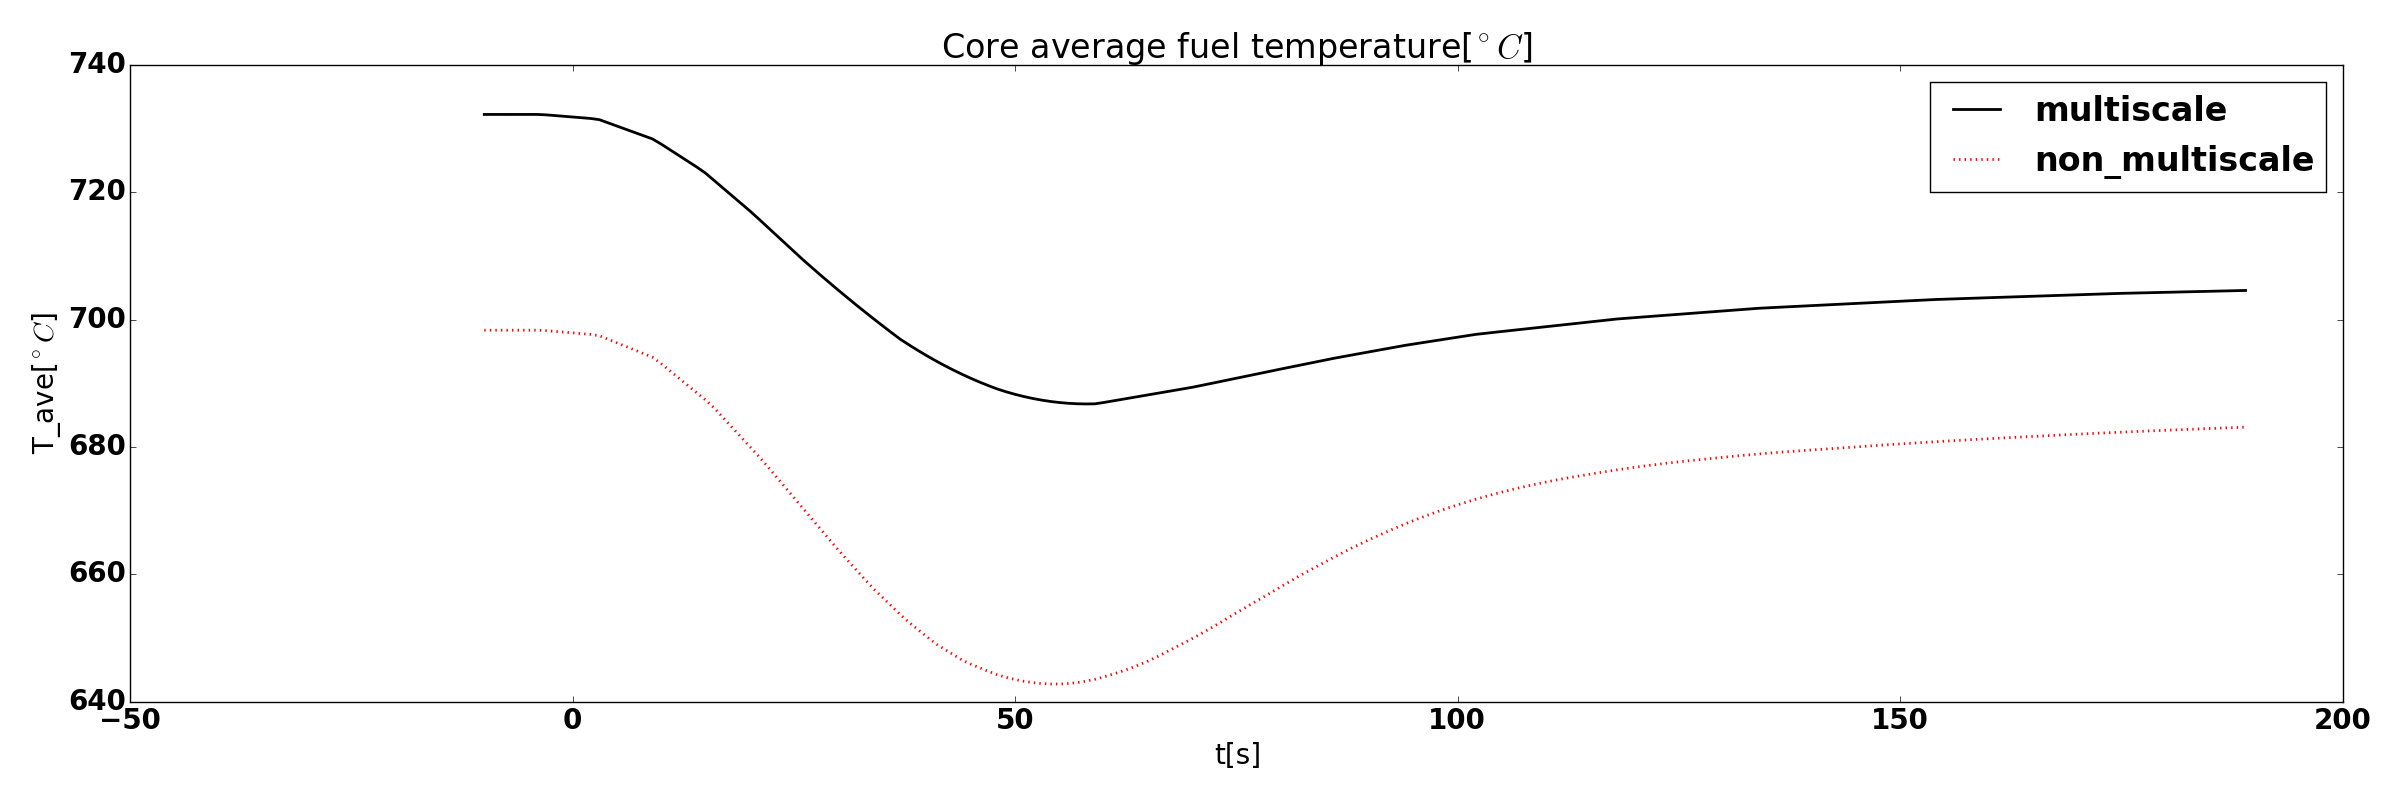
\includegraphics[width=1\textwidth]{./images/diffusion/tmsr/OC/compare_multiscale/T_fuel_ave.png}
        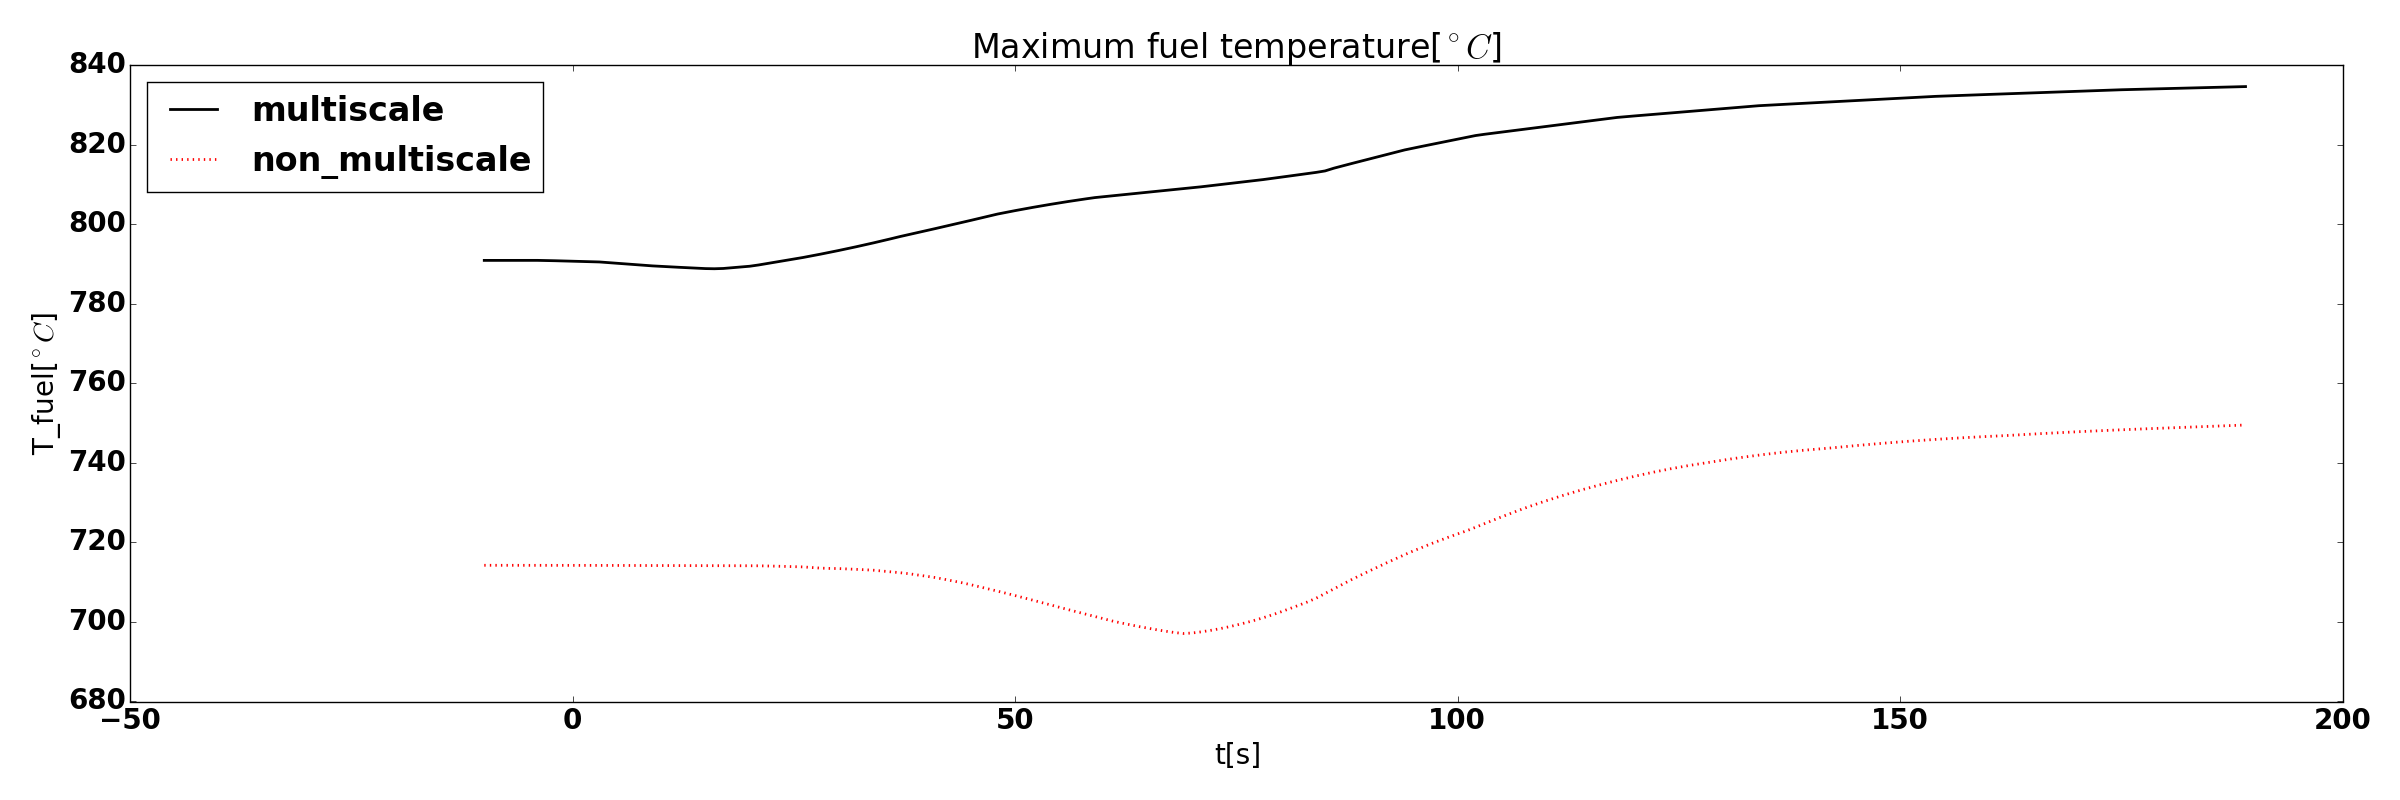
\includegraphics[width=1\textwidth]{./images/diffusion/tmsr/OC/compare_multiscale/T_fuel_max.png}

        \caption{Core average and maximum fuel temperature during overcooling transient}
        \label{fig:tmsr_oc_fuel}
\end{figure}


\begin{figure}
    \centering
    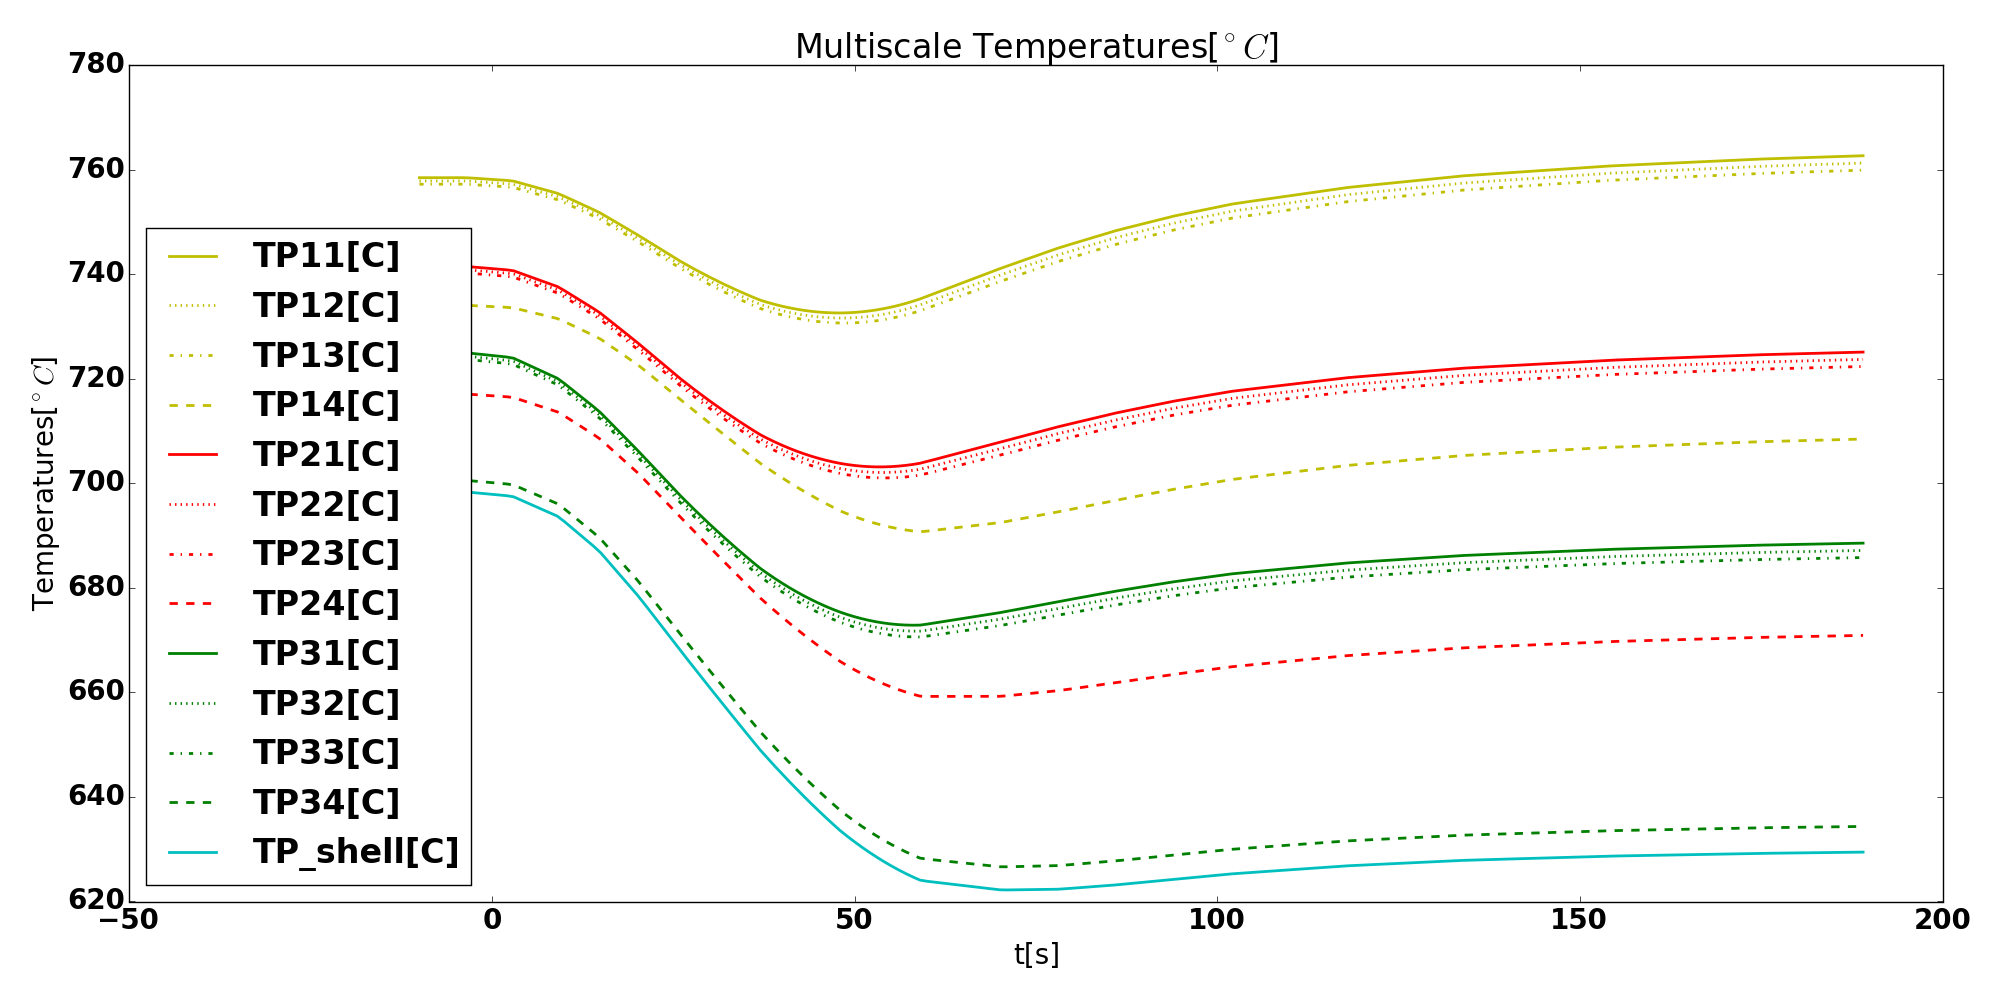
\includegraphics[width=\textwidth]{images/diffusion/tmsr/OC/compare_multiscale/temps.png}
    \caption{Core average of temperatures inside fuel pebbles during overcooling transient for TMSR SF-1. Notation for temperatures: $TP_{ij}$ represents the ith TRISO layer in the jth pebble layer. $TP_{shelll}$ is the temperature in the graphite shell of the pebble.}
    \label{fig:temps_OC_tmsr}
\end{figure}


Starting from the steady state conditions (section \ref{sec:TMSR_SS}), the inlet coolant temperature is decreased by 100$^{\circ}C$ in 10 seconds and remains at the lower level during the simulated overcooling transient. Within the short timescale of the simulation, it is reasonable to assume that the other inlet conditions (e.g. coolant mass flow rate) and the reactor control parameters (e.g. control rod positions) remain unchanged. 

The colder coolant introduces positive reactivity insertion due to negative flibe temperature reactivity feedback, which causes a power increase, as shown in figure \ref{fig:OC_power}. The increase is slow at the beginning because the temperature reactivity feedback is mainly from the coolant, weaker then the Doppler feedback from the fuel, which comes into effect after about 10 seconds when the cooling reaches the fuel materials. 
Because the transient is initiated in the coolant, the multiscale power increases less than that in the model with uniform fuel temperature, because it can capture the feedback from fuel while the fuel material gets cooled gradually from the shell to the center kernel.
The change in temperature in turn results in  negative reactivity feedback that stabilize the power at a higher level than the initial rate. 

Figure \ref{fig:tmsr_oc_flibe} shows that both the average and maximum coolant temperature drops at first due to the colder inlet and increase later due to the increased power.
The average coolant temperature drops immediately due to the decreased inlet temperature. 
On the other hand, the maximum coolant temperature, which is also the outlet temperature, is not affected until the colder coolant arrives at the top of the core. This parameter is directly related to the hot-leg temperature and determines the reactor safety margin. However, this is not a safety concern for over-cooling transients where the coolant temperature is below the steady state condition. 

Figure \ref{fig:tmsr_oc_fuel} shows the variation of both the maximum and the average fuel temperature during the transient, with two different models.
The average fuel temperature drops with the coolant, heats up from the reactivity feedback and in the end stabilizes at a lower level than the steady state temperature.
The location where the fuel temperature peaks changes from the center of the core to the top as the coolant flows through the core. At the end of the transient, the peak fuel temperature is higher than the steady state temperature despite the colder coolant that flows through the core, but is still well below the safety limit. 
Both the average and the maximum fuel temperature in the core is higher with the multiscale treatment, because it captures the feedback from the fuel correctly. 

Overall, the end state of the fuel temperature is lower while the coolant temperature is higher in the non-multiscale model because it overestimates the contribution to the negative reactivity feedback from the coolant. 
In fact, the estimated maximum flibe temperature in this case is much higher than in the multiscale case, even higher than the steady state value. This may lead to over conservatism in the design. 


If we take a closer look at the temperature profile inside the fuel pebbles during the transient, figure \ref{fig:temps_OC_tmsr} shows the temperature in each solid layer at each time stamp.
It takes a few seconds for the drop in the inlet coolant temperature to affect the solid temperature. The core-wise average temperatures in the fuel elements decrease at first as the cold coolant flows upward in the core.
At around 50 second, the temperatures increase due to the surge in power. The temperatures finally stabilize after about 150 seconds. The surface temperature is much lower than the steady state temperature because the coolant temperature is much lower.
The temperatures gradient inside a fuel pebble is higher after the transient because the power is at a higher level. The difference between the hottest layer and the shell changed from 60 K to 130 K after the transient. As a result, the inner most layer has a slightly higher temperature after the transients, although the safety margin to fuel damage is still very large. 






\newpage

\section{Conclusion}

In this section, a coupled thermal-hydraulics and neutronics model for the TMSR SF-1 is developed, verified against a reference model, and then used to perform steady state and transient computation. The model provides high resolution two dimensional or three dimensional results within a reasonable amount of time on a computer with 16.0 GB RAM and four Intel Core equipped with i7-4790K CPU at 4.00 GHz.

Steady state parameters such as power, temperatures and neutron flux are calculated and discussed. The large safety margins to fuel damage or coolant boiling at steady state make the core robust to various transients. 
The fuel and coolant temperature during a 1\$ reactivity insertion is within the safety limit.
Likely, during the overcooling transient, where the coolant inlet temperature is dropped by 100 \degc\ in 10 seconds, the core-wise maximum fuel temperature is 950$^{\circ}C$, largely below the safety limit for fuel element. The coolant temperature stabilizes at a lower level than the initial condition, but is still above the salt freezing point.

In conventional porous media formulation, only an average temperature inside the solid phase is computed. This is a reasonable assumption in steady state cases and in most slow transient problems where the fuel kernel temperature is very close to the temperature of the surrounding graphite matrix. However, in the case of fast transients involving large power excursions, the difference between fuel and graphite temperatures can be significant. Thus a detailed temperature profile inside the fuel pebbles and TRISO fuel kernels is necessary for accurately computing temperature, which is important in capturing the Doppler temperature reactivity feedback. %Heat transfer inside the TRISO particles can be assumed to be isotopic. 
Overall, the power excursion in response to either a large reactivity insertion or a overcooling transient is dampened when a temperature profile in the fuel element is used, because the temperature reactivity feedback is captured more realistically at the place where the largest feedback occurs. 

















\subsection{Transient results}
The coupled model has the capability of simulating both steady state and transients by determining the time dependent spatial flux distribution and flow field conditions. Reactivity insertion transients and overcooling transients are discussed in this section.





\subsubsection{Reactivity insertion transient results}
Reactivity insertion can happen in a reactor core when one or more control rods are extracted inadvertently. FHRs do not have the risk of control rod ejection because of its low operating pressure, but are under the risk of reactivity insertion associated with the seismic compression of the fuel bed.

Only the core is included in the model, the change in inlet and outlet conditions is not simulated for these fast transients. In fact, most of the heat is trapped in the fuel particles, does not have time to induce significant changes beyond the core.

\begin{figure}[ht]
    \centering
    \begin{subfigure}[b]{0.45\columnwidth}
        \centering
        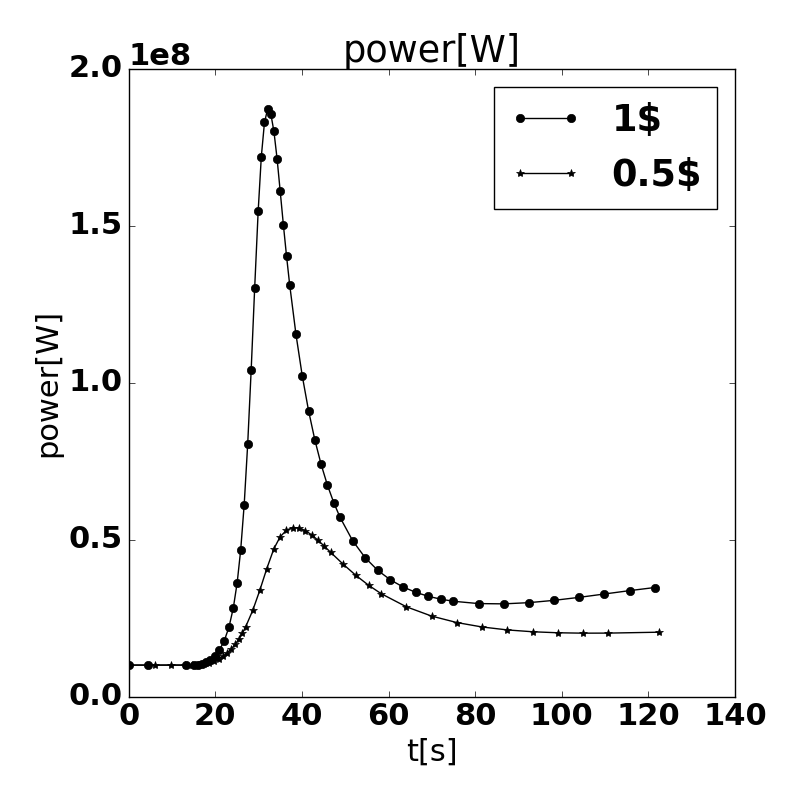
\includegraphics[width=0.9\textwidth]{./images/diffusion/RI/power_diff_pcm.png}
        \caption{Power}
    \end{subfigure}%
    ~
    \begin{subfigure}[b]{0.45\columnwidth}
        \centering
        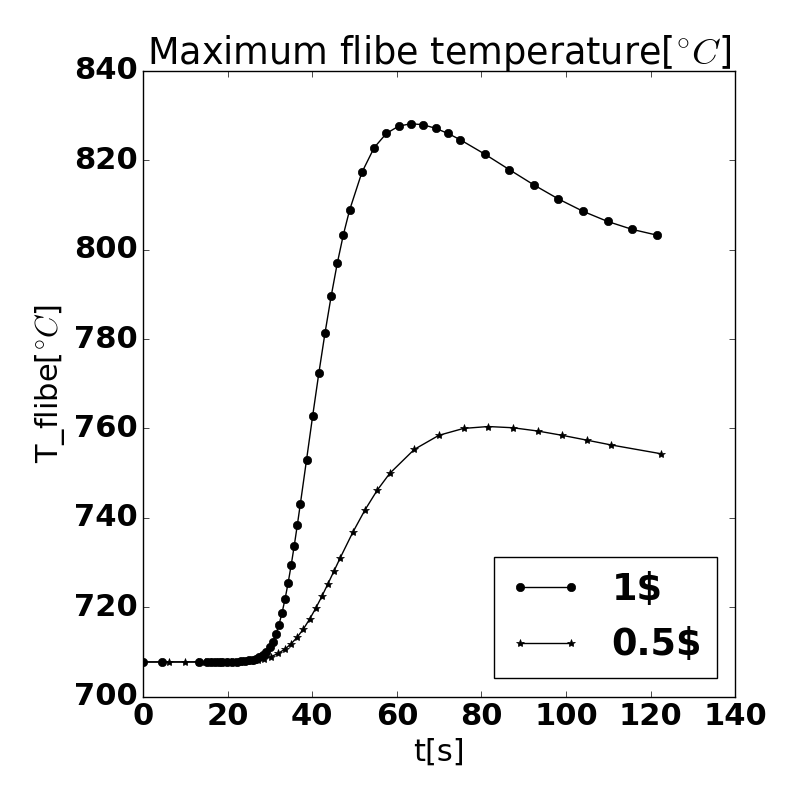
\includegraphics[width=0.9\textwidth]{./images/diffusion/RI/T_flibe_max_diff_pcm.png}
        \caption{Maximum core-wise flibe temperature}
    \end{subfigure}
    ~
    \begin{subfigure}[b]{0.45\columnwidth}
        \centering
        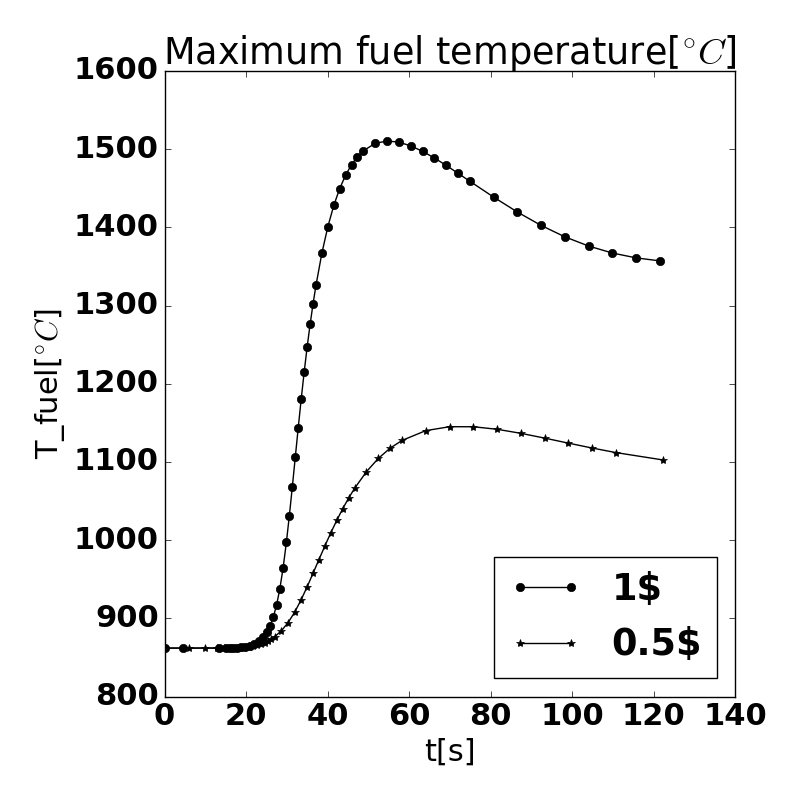
\includegraphics[width=0.9\textwidth]{./images/diffusion/RI/T_fuel_max_diff_pcm.png}
        \caption{Maximum core-wise Fuel temperature}
    \end{subfigure}
    \caption{RI transients}
    \label{fig:RI}
\end{figure}


Figure \ref{fig:RI} shows the RI transients results. At the onset of the transient, nuclear power increases due to excess of reactivities. Consequently, the fuel temperature increases too and then the flibe temperature, both providing negative temperature reactivity feedback that stabilize the reactivity in the core. 
The negative temperature reactivity feedback is the most important safety mechanism for the core stablization during reactivity insertion without SCRAM transients. The Doppler feedback in the fuel due to resonance absorption is much more prominent in FHR cores than the coolant void feedback.

The power is releveled at a higher rate at the end of this two-minutes transient. During the 1\$ prompt insertion transient, the core maximum fuel temperature is 1500$^{\circ}$C, below the safety limit (1600$^{\circ}$C). 
Coolant temperature is raised by only 100$^{\circ}$C at the peak. 






\subsubsection{Overcooling transients}
Overcooling transients occur when cold coolant is injected in the core due to check valve opening or other anomalies. Due to the high melting point of the coolant, understanding the core behavour under overcooling transients is important in FHRs to prevent salt freezing that could potentially block the circulation and cause major damages.

 The cold coolant introduces positive reactivity insertion due to negative flibe temperature reactivity feedback. The increased power causes an elevation in the fuel temperature, which in turn introduces negative reactivity that stabilize the core. 

A decrease in inlet coolant temperature of 100$^{\circ}C$ in 10 seconds is simulated while other parameters such as mass flow rate, pressure drop, control rod positions remain unchanged. The temperature and power evolution during the overcooling transient is shown in Figure \ref{fig:OC}. At the 50th second, the inlet coolant temperature starts to drop and the fuel temperature and power increases. At the end of the transient, the core-wise maximum fuel temperature is 950$^{\circ}C$. 

\begin{figure}[h!]
    \centering
    \begin{subfigure}[b]{0.45\columnwidth}
        \centering
        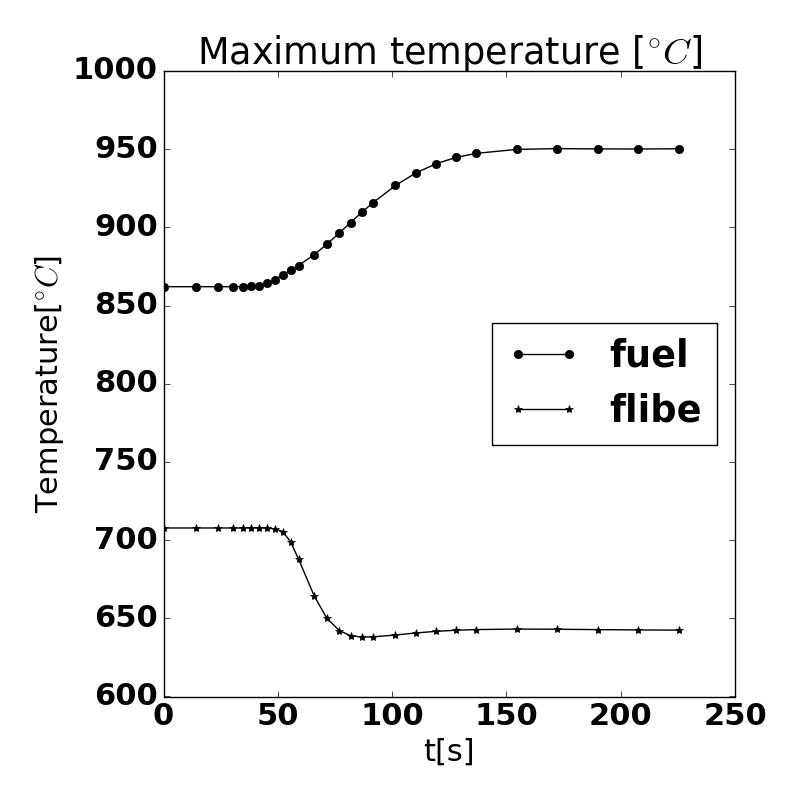
\includegraphics[width=0.9\textwidth]{./images/diffusion/OC/T_fuel_flibe_max.png}
        \caption{Maximum fuel and flibe temperature}
    \end{subfigure}%
    ~
    \begin{subfigure}[b]{0.45\columnwidth}
        \centering
        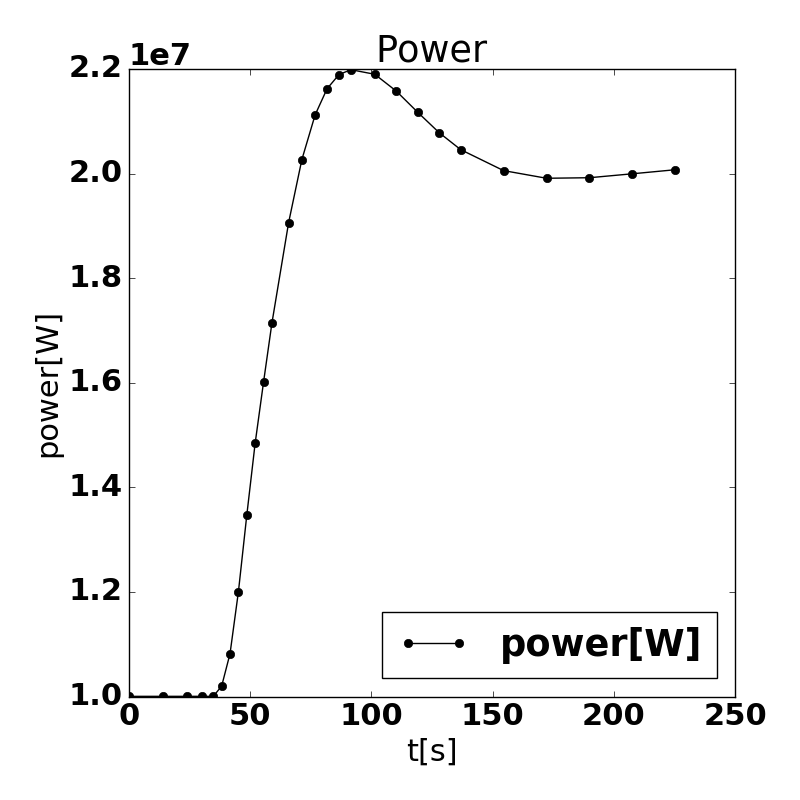
\includegraphics[width=0.9\textwidth]{./images/diffusion/OC/power.png}
        \caption{Power}
    \end{subfigure}
    \caption{Overcooling transient results}
    \label{fig:OC}
\end{figure}






\section{Conclusion}
Strict safety requirement for next-generation reactors along with the progress in computer technology prompts the development, qualification and application of time-dependent multi-physics models for FHRs.
In this paper, a coupled neutronics/thermal-hydraulics model for FHRs is described. It utilizes COMSOL Multiphysics to solve for neutron diffusion, delayed neutron precursor concentration equations and porous media CFD. Benchmarking with the Monte Carlo based model shows satisfying agreement. 

Although the results discussed in this paper are based on a specific FHR design - the TMSR, the methodology can be used for all pebble bed FHRs.

Steady state and transient results of power, temperatures and neutron flux are discussed in this paper. The use of thermal resistant TRISO fuel, flibe coolant and graphite reflectors renders the core extremely robust against accidents. 
Because of the use of highly robust elements in the core, failures due to high temperature would be more likely to occur at the hot legs outside the core.
This model can provide input conditions to structure analysis for metallic structures, the most vulnerable elements in the core. 


The Biot number of the fuel pebble is approximately 9.4, using the nominal pebble bed heat transfer coefficient(4700 $W/m^2K$), a nominal equivalent thermal conductivity estimation of the FHR fuel pebble(15 W/m.K), the diameter of a fuel pebble in MK1(0.03m) and the formular in equation \ref{eq:biot}.
\begin{equation}
    Bi = \frac{hD}{k}
    \label{eq:biot}
\end{equation}
Therefore the radial variation of temperaure in the pebble is not negligible compared to that in the coolant.
The temperature profile inside fuel pebbles and TRISO particles is especially important for acute transients such as the reactivity insertion transients, during which the heat does not have time to escape from the fuel structure. While it is not feasible to model the temperature of each of the millions of TRISO particles in an FHR core, it is indispensable to implement appropriate multi-scale treatment to approximate the fuel temperature during a reactivity-induced transient.

Simplified spherical harmonics algorithm will be implemented to account for the asymmetry in neutron transport, especially near the boundaries and strong absorbers like control rods.


\section*{References}

\bibliography{references}

\end{document}
